\chapter{Lie Algebras}
\section{Facts from linear algebra}
\subsection{Jordan Normal form}
Here will denote $X:V\rightarrow V$ an endomorphism.\par
Some important facts:
\begin{itemize}
    \item Let $f,g\in\mathbb{C}[t]$ be such that $f\cdot g(X)=0, \gcd(f,g)=1$. Then 
    \begin{equation}
        V = \text{Ker}f(X)\oplus \text{Ker}g(X).
    \end{equation}
    \item Let $p$ be the characteristic polynomial of $X$ and 
    \begin{equation}
        p(t)=\prod_{i=1}^r(t-a_i)^{m_i}
    \end{equation}
    be its factorization. Then 
    \begin{equation}
        V = \bigoplus_{i=1}^r\text{Ker}(X-a_i\mathds{1}_V)^{m_i}.
    \end{equation}
    \item $v\in V\setminus0$ is said to be $(X-a\mathds{1})-$cyclic with period $r$ if 
    $(X-a\mathds{1})^{r-1}v\neq0$ while $(X-a\mathds{1})^rv=0$. In this case the set
    \begin{equation}
        v,\;(X-a\mathds{1}_V)v,\dots,\;(X-a\mathds{1}_V)^{r-1}v
    \end{equation}
    is linearly independent.
\end{itemize}

\begin{dang}
\begin{theorem}
 (Jordan normal form).   $V$ is the direct sum of $X$-cyclic subspaces, i.e., $A$-invariant subspaces with a basis of the form 
    \begin{equation}
        v,\;(X-a\mathds{1}_V)v,\dots,\;(X-a\mathds{1}_V)^{r-1}v
    \end{equation}
    for some $v\in V\setminus0,a\in\mathbb{C},r\geq1$.
\end{theorem}
\end{dang}
Proof (sketch): Let $p$ be the characteristic polynomial of $X$ with unique factorization 
\begin{equation}
    p(t)=(t-a_1)^{m_1}\cdots(t-a_r)^{m_r}.
\end{equation}
Then we know that 
\begin{equation}
    V = \bigoplus_{i=1}^r\text{Ker}(X-a_i\mathds{1}_V)^{m_i}.
\end{equation}
Restriction to $V_i =\text{Ker}(X-a_i\mathds{1}_V)^{m_i}$ yields the additional hypothesis: We can assume that there exist 
$a\in\mathbb{C}$ and $m\geq1$ such that 
\begin{equation}
    (X-a\mathds{1}_V)^m=0.
\end{equation}
Now we solve the problem inductively:
\begin{itemize}
    \item Write $B=X-a\mathds{1}_V$ and let $m\geq1$ be the smallest integer such that $B^m=0$. Then there exist 
    $v\in V\setminus0$ such that $B^{m-1}v\in\text{Ker}(B)\setminus0$. Therefore
    \begin{equation}
        \text{dim}(BV)<\text{dim}(V).
    \end{equation}
    \item by induction, we have a decomposition
    \begin{equation}
        \begin{split}
             &BV = W_1\oplus \cdots\oplus W_k, \\
             &W_i=\langle w_i,\cdots B^{r_i-1}w_i \rangle
        \end{split}
    \end{equation}
    into cyclic $X$-invariant subsapces.
    \item Let $v_i\in V$ be such that $Bv_i=w_i$, then 
    \begin{equation}
        V_i=\langle v_i,\dots, B^{r_i}v_i\rangle.
    \end{equation}
    Now we write $V^\prime = V_1\oplus\cdots\oplus V_k$ and complete it to a basis of $V$ using elements of $\text{Ker}(B)$.
\end{itemize}
\qed

\begin{dang}
    \begin{example}
        Find the Jordan Normal form of the matrix:
        \begin{equation}
         X=\begin{pmatrix}
                1&2&-1\\ 0&1&\;\;1\\ 0&0&\;\;1
            \end{pmatrix}
        \end{equation}
    \end{example}
\end{dang}



\begin{dang}
    \begin{remark}
        Let $A\in M_n(\bbC)$ and $p\in\bbC[t]$ its associated characteristic polynomial. If
        \begin{equation}
            p(t)=\prod_{i=1}^r(t-\lambda_i)^{m_i},\;\lambda_i\neq\lambda_j
        \end{equation}
        then the number $m_i$ is called \textit{algebraic multiplicity} of $\lambda_i$. It has the property 
        \begin{equation}
            m_i=\dim\Ker(A-\lambda_i I)^{m_i}.
        \end{equation}
    \end{remark}
\end{dang}
We have a general property: $\Ker(A-\lambda_i I)^k\overset{\neq}{\subset}\Ker(A-\lambda_i I)^{k+1}$ for $k=1,\dots,m_i-1$ while 
$\Ker(A-\lambda_i I)^{N}=\Ker(A-\lambda_i I)^{m_i},\;N\geq m_i$. 

\begin{dang}
    \begin{definition}
        If $X\in\End(V)$, then we define the \textit{generalized eigenspace}
        \begin{equation}
            V_\lambda^X=\{v\in V: (X-\lambda\mathds{1}_V)^Nv=0,\;\text{ for some }N\geq1\}.
        \end{equation}
    \end{definition}
\end{dang}
Of course, if $V_\lambda^X\neq0$, then $\lambda$ is an eigenvector of $X$ and by the previous discussion 
\begin{equation}
    V_\lambda^X = \Ker(X-\lambda\mathds{1}_V)^m
\end{equation} 
where $m$ is the algebraic multiplicity of $\lambda$.

\subsection{Jordan Chevalley decomposition}
\begin{dang}
    \begin{remark}
        A endomorphism $X$ is semisimple if for any $X-$invariant subspace $W$, we can find a $X$-invariant complement
        $W^\prime$. So we have the decomposition into $X$-invariant subspaces:
        \begin{equation}
            V = W\oplus W^\prime.
        \end{equation}
    \end{remark}
\end{dang}
Since we are working in $\mathbb{C}$, semisimplicity is equivalent to $X$ being diagonalizable. In fact, if $X$ is 
semisimple, let $v\in V\setminus0$ be an eigenvalue. Then $\mathbb{C}v$ is $X$-invariant and there exist a $X$-invariant 
subspace $X$ such that $V=\mathbb{C}v\oplus W$. Now, induction finnnish the job. Conversely, if $X$ is diagonalizable, let 
$v_1,\dots,v_n,\;n=\text{dim}(V)$ be a basis consisting of eigenvectors of $X$. Since $V=W+\langle v_1,\dots, v_n\rangle$, we can 
find $v_{i_1},\dots, v_{i_s}$ such that $V=W\oplus \langle v_{i_1},\dots, v_{i_s}\rangle$.

\begin{dang}
    \begin{remark}
        The chinese remainder theorem, in the case of polynomials is the statement that 
         if $f=g_1\cdots g_r,\;\gcd(g_1,\dots,g_r)=1$, then 
        \begin{equation}
            h+(f) \overset{\cong}{\longmapsto} (h+(g_1),\dots,h+(g_r))
        \end{equation}
        is an isomorphism.
    \end{remark}
\end{dang}
By the previous remark, solving a system of congruences:
\begin{equation}
    \begin{split}
        &f = a_1 \text{ mod } g_1\\
        &\cdots\\
        &f = a_r \text{ mod } g_r
    \end{split}
\end{equation}
is just a linear algebra problem.
\begin{dang}
    \begin{example}
      Find a solution to:
      \begin{equation}
        \begin{split}
            &f = 2t+1\text{ mod }t^2+1\\
            &f = 4 \text{ mod } t-1
        \end{split}
      \end{equation}
    \end{example}
\end{dang}
First we see that $\gcd(t^2+1,t-1)=1$ and if $f=(t^2+1)(t-1)$, then
\begin{equation}
   T: h+(f)\mapsto (h+(t^2+1),h+(t-1))
\end{equation}
is an isomorphism. We have the basis $1+(f),t+(f),t^2+(f)$ of $\mathbb{C}[t]/(f)$, $1+(t^2+1),t+(t^2+1)$ of 
$\mathbb{C}[t]/(t^2+1)$ and $1+(t-1)$ of $\mathbb{C}[t]/(t-1)$. With respect to these basis, $T$ has matrix expression
\begin{equation}
   X= \begin{pmatrix}
        1&0&-1\\ 0&1&\;\;0\\ 1&1&\;\;1
    \end{pmatrix}.
\end{equation}
Now, to solve the system of congruences, we solve the linear system $Xv=(1,2,4)^T$ which gives $v=(3/2,2,1/2)$, or 
\begin{equation}
    f = \frac12 t^2+2t+\frac32.
\end{equation}

\begin{dang}
    \begin{theorem}
        (Jordan - Chevalley decomposition). Let $X\in\text{End}(V)$.
        \begin{itemize}
            \item[(1)] We have a (unique) decomposition $X=X_s+X_n$ into a semisimple and a nilpotent element such that 
            $[X_s,X_n]=0$.
            \item[(2)] Both $X_s,X_n$ are polynomials in $X$ without constant terms.
        \end{itemize}
    \end{theorem}
\end{dang}
Proof: As before, if $p$ is the characteristic polynomial of $X$ with factorization $p=\prod_{i=1}^r(t-a_i\mathds{1})^{m_i}$. 
Then $V=\bigoplus_{i=1}^rV_i,\;V_i=\text{Ker}(X-a_i\mathds{1})^{m_i}$. Now we solve a system of congruences:
\begin{itemize}
    \item If exist $a_i=0$:
    \begin{equation}
        \begin{split}
            & f = a_1 \text{ mod } (t - a_1)^{m_1}\\
            &\cdots\\
            & f = a_r \text{ mod }(t-a_r)^{m_r}
        \end{split}
    \end{equation}
    \item If $a_i\neq0,\;\forall i$, then we add the equation $f=0\text{ mod }t$ to the previous system.
\end{itemize}

Now, it's clear that $f(X)|_{V_i}=a_i\mathds{1}_{V_i}$, and $f(X)$ is diagonalizable. Furthermore, if $g(t)=t-f(t)$, then 
$g(X)|_{V_i}= X-a_i\mathds{1}\big|_{V_i}$ which is nilpotent with index $m_i$. Taking $m = m_1\cdots m_r$ we see that 
$g(X)^m=0$, so $g(X)$ is a nilpotent operator. Now we just define $X_s=f(X)$ and $X_n=g(X)$. 


\begin{dang}
    \begin{lemma}
        Let $X\in\text{End}(V)$, then $\ad(X_s)=\ad(X)_s$ and $\ad(X_n)=\ad(X)_n$.
    \end{lemma}
\end{dang}
Prood: Recall that $\ad(X)=L_X-R_X$, where $L_X(Y)=XY,R_X(Y)=YX$. It's clear that $L_X,R_X$ commute and are nilpotent if
$X$ is nilpotent. Therefore $\ad(X)$ is nilpotent if $X$ is nilpotent. Furthermore, if $X$ is semisimple,
choose an eigenbasis $v_1,\dots, v_n$ and let $E_{ij}:v_k\mapsto v_{jk}v_i$. Then we see that 
\begin{equation}
    \ad(X)E_{ij}v_k = \delta_{kj}a_i v_i-a_k\delta_{kj}v_i = (a_i-a_j)E_{ij}v_k.
\end{equation}
So $\ad(X)E_{ij}= (a_i-a_j)E_{ij}$ and $\ad(X)$ is diagonalizable. By uniqueness of Chevalley decomposition we see prove the 
statement.\qed

\section{Engel and Lie theorems}
\begin{dang}
    \begin{theorem}
        (Engel's theorem). If $\fr{g}\subset\End(V)$ consisting of nilpotent endomorphisms, then there exist 
        $v\in V\setminus0$ such that $Xv=0,\;\forall X\in\fr{g}$. Furthermore, this means that we can find a basis such that 
        \begin{equation}
            \fr{g}\subset \fr{t}_n=\left\{
                \begin{pmatrix}
                    0&*\\
                    0&0
                \end{pmatrix}
            \right\}
        \end{equation}
    \end{theorem}
\end{dang}
Proof: The strategy of the proof is the following:
\begin{itemize}
    \item Apply induction on dimension of $\fr{g}$ to show that there exist a codimension 1 ideal $\fr{h}\subset\fr{g}$.
    \item Apply induction of dimension of $\fr{h}$ to conclude that $W=\{v\in V: Xv =0,\;\forall X\in\fr{h}\}\neq0$. 
    In this case, any $Y\in\fr{g}$ outside $\fr{h}$ restricts to $W$ and we finnish the proof using the fact that $Y$ is 
    nilpotent.
\end{itemize}
The candidate for a codimension 1 ideal in $\fr{g}$ is any maximal (proper) subalgebra $\fr{h}\subset \fr{g}$. Now, 
$\fr{g}/\fr{h}$ is a vector space with the adjoint action of $\fr{h}$. In particular $\ad(X)$ acts nilpotently as an 
element in $\End(\fr{g}/\fr{h})$ and by the induction hypothesis there exist $Y\in\fr{g}$ such that 
$\ad(\fr{h})Y\subset\bbC Y$. Therefore $\fr{h}\oplus\bbC Y\subset\fr{g}$ is a subalgebra. By the maximality assumption, we have 
$\fr{g}=\fr{h}\oplus\bbC Y$.\par 

Now, let $W=\{v\in V: Xv =0,\;\forall X\in\fr{h}\}$ which is nonzero if we apply the induction hypothesis again for 
$\dim(\fr{h})$. So, to finnish the proof we just need $v\in W,\;Yv=0$. Let $v\in V$, then 
\begin{equation}
    XY(v) = YX(v)+[X,Y](v)\overset{[X,Y]\in\fr{h}}{=}YX(v)\overset{X\in\fr{h}}{=}0,\;\forall X\in\fr{h}.
\end{equation}
Therefore $Y(v)\in W$, i.e., $Y|_W\in\End(W)$ is a nilpotent endomorphism. So we can find $w\in W\setminus0$ such that 
$Y(w)=0$.\qed

\begin{dang}
    \begin{remark}
       By just reading the definition, the condition of $\fr{g}$ being nilpotent looks stronger than the condition of each 
        $\ad(X),\;X\in\fr{g}$ being a nilpotent endomorphism of $\fr{g}$. However, by Engel's theorem, the two conditions 
        are the same. In fact, if every $\ad(X)$ is nilpotent, then $\ad(\fr{g})$ is a nilpotent subalgebra of $\fr{gl}_\fr{g}$
        and by Engel's theorem $\ad(\fr{g})\subset\fr{n}_n$ for some choice of basis of $\fr{g}$. This says that $\ad(\fr{g})$ is nilpotent
        and thus $\fr{g}/Z(\fr{g})$ is nilpotent, which implies $\fr{g}$ nilpotent. 
    \end{remark}
\end{dang}

\begin{dang}
    \begin{remark}
        (Be careful !) If $\fr{g}\subset\End(V)$ we is a nilpotent Lie subalgebra, then we can not immediately 
        apply Engel's theorem, because we need that $\fr{g}$ be a subalgebra consisting of nilpotent endomorphisms of $V$.
    \end{remark}
\end{dang}

\begin{dang}
    \begin{lemma}
        (Weight spaces are invariant). 
        Let $\fr{h}\subset\fr{g}$ an ideal, $V$ a representation of $\fr{g}$ and $\lambda\in\fr{h}^*$. Then 
        $V_{\fr{h}}^\lambda = \{v\in V: X(v)=\lambda(X)v,\;\forall X\in\fr{h}\}$ is $\fr{g}-$invariant.
    \end{lemma}
\end{dang}
Proof: Let $w\in W=V_{\fr{h}}^\lambda, Y\in\fr{g}$ and define $U=\langle w,Y(w),Y^2(w),\dots \rangle$. This is clearly a $Y-$invariant 
subspace. We also claim that this is a $\fr{h}-$invariant subspace. In fact, for $X\in\fr{h}$ we have $Xw=\lambda(X)w$, 
\begin{equation}
XY(w)=YX(w)+[X,Y](w)\overset{[X,Y]\in\fr{h}}{=}\lambda(X)Y(w)+\lambda([X,Y])w \in U
\end{equation} 
and in general, $XY^k(w)\in U$ can be proved by induction. In particular we see that $X|_W$ is triangular, with trace 
$\lambda(X)\dim(W)$. Finnaly, with this observation we see that 
\begin{equation}
    \lambda([X,Y])\dim(W)=\Tr([X,Y]|_W)=0\Rightarrow \lambda([X,Y])=0.
\end{equation}
Therefore, we see that $XY(w)=\lambda(X)Y(w)$, i.e., $Y(w)\in W$.\qed

\begin{dang}
    \begin{theorem}
        (Lie theorem).
        If $\fr{g}\subset\End(V)$ is a solvable Lie subalgebra, then there exist $v\in V\setminus0$ fixed by $\fr{g}$. 
        This means that we can find a basis of $V$ such that 
        \begin{equation}
            \fr{g}\subset \fr{b}_n=\left\{\begin{pmatrix}
                *&*\\0&*
            \end{pmatrix}\right\}.
        \end{equation}
    \end{theorem}
\end{dang}
Proof: The strategy here is the following:
\begin{itemize}
    \item Apply induction on $\dim(\fr{g}/[\fr{g},\fr{g}])$ to conclude that there exist a codimension 1 ideal in $\fr{g}$.
    \item Apply induction again to to find a nonzero vector $v$ fixed by $\fr{h}$ and finnish the proof.
\end{itemize}

Since $\fr{g}$ is solvable, $[\fr{g},\fr{g}]$ is proper ideal in $\fr{g}$. So $\fr{g}/[\fr{g},\fr{g}]$ is a nonzero 
abelian Lie algebra. By induction, there exist a codimension 1 ideal $\fr{a}\subset \fr{g}/[\fr{g},\fr{g}]$. If 
$\pi^{-1}(\fr{a})=\fr{h}$, then $\fr{h}/[\fr{g},\fr{g}]= \fr{a}$ and 
\begin{equation}
    \dim(\frac{\fr{g}/[\fr{g},\fr{g}]}{\fr{a}})
    =\dim(\frac{\fr{g}/[\fr{g},\fr{g}]}{\fr{h}/[\fr{g},\fr{g}]})=\dim(\fr{g}/\fr{h}).
\end{equation}
Therefore, $\fr{h}$ is a codimension 1 ideal in $\fr{g}$. Let $Y\in\fr{g}$ be such that $\fr{g}=\fr{h}\oplus\bbC Y$. 
By the induction hypothesis, there exist $v\in V\setminus0$ fixed by $\fr{h}$, i.e., $W=V_{\fr{h}}^\lambda\neq0$ 
for some $\lambda\in\fr{h}^*$. Finnaly, by the previous lemma $Y|_W\in\End(W)$, so we just take $w$ an eigenvector of 
$Y|_W$.\qed

\begin{dang}
    \begin{remark}
        Lie's theorem is easier to apply than Engel's theorem because the condition lies entirely the 
        Lie subalgebra itsel (i.e., its solvability condition), not in its action on $V$.
    \end{remark}
\end{dang}



\section{Semisimplicity criterions}
The two main theorems of this section is the Cartan criteria for semisimple and solvable Lie algebras.
All necessary definitions follows after the statement of the theorem.
\begin{dang}
    \begin{theorem}\label{theorem: CC(ss)}
        (CC(ss)).
         Cartan criteria for semisimple Lie algebras: 
        A Lie algebra $\fr{g}$ is semisimple if and only if the Killing form $K^{\fr{g}}$ is nondegenerate. 
    \end{theorem}
\end{dang}

\begin{dang}
    \begin{theorem}\label{theorem: CC(sol)}
        (CC(sol)).
        Cartan criteria for solvable Lie algebras: A Lie algebra $\fr{g}$ is solvable if and only if 
        $K^{\fr{g}}(\fr{g},[\fr{g},\fr{g}])=0$.
    \end{theorem}
\end{dang}


Some key definitions that we need:
\begin{itemize}
    \item Central series of a Lie algebra: Is the decreasing sequence of ideals $\fr{g}^k$ defined by
    \begin{equation}
        \left\{\begin{matrix}
            &\fr{g}^0=\fr{g},\\
            &\fr{g}^k=[\fr{g},\fr{g}^{k-1}],k\geq1.
        \end{matrix}\right.
    \end{equation}
    \item Derived series of a Lie algebra: Is the decreasing sequence of ideals $\fr{g}^{(k)}$ defined by
    \begin{equation}
        \left\{\begin{matrix}
            &\fr{g}^{(0)}=\fr{g},\\
            &\fr{g}^{(k)}=[\fr{g}^{(k-1)},\fr{g}^{(k-1)}],k\geq1.
        \end{matrix}\right.
    \end{equation}
    \item A Lie algebra is said to be \textit{nilpotent} if its central series
    \begin{equation}
       \fr{g}\supset \fr{g}^1\supset\cdots\supset\fr{g}^k= 0
    \end{equation}
    terminates at 0.

    \begin{dang}
        \begin{remark}
            An equivalent definition of nilpotent Lie algebras is the following one: There exist a chain of ideals 
            \begin{equation}
                 \fr{g}_0=\fr{g}\supset\fr{g}_1\supset\cdots\supset\fr{g}_k=0
            \end{equation}
            such that $\fr{g}_i/\fr{g}_{i+1}\in Z(\fr{g}/\fr{g_{i+1}})$.
        \end{remark}
    \end{dang}
    In fact, if it's the case, then we claim that $\fr{g}^i\subset \fr{g}_i,\;i\geq0$. For $i=0$ it's just the 
    definition. Now, in general 
    \begin{equation}
        \fr{g}^{i+1}=[\fr{g},\fr{g}^{i}]\overset{\fr{g}^{i}\subset\fr{g}_i}{\subset}[\fr{g},\fr{g}_{i}]
        \overset{\fr{g}_i/\fr{g}_{i+1}\in Z(\fr{g}/\fr{g_{i+1}})}{\subset}\fr{g}_i
    \end{equation}
    which shows that the central series terminates in zero.


    
    \item A Lie algebra is said to be \textit{solvable} if its derived series
    \begin{equation}
       \fr{g}\supset \fr{g}^{(1)}\supset\cdots\supset\fr{g}^{(k)}=0
    \end{equation}
    terminates at 0.
    \begin{dang}
        \begin{remark}
            An equivalent definition for solvable Lie algebras: There exist a sequence of \textit{Lie subalgebras} 
            \begin{equation}
                \fr{g}_0=\fr{g}\supset\fr{g}_1\supset\cdots\supset\fr{g}_k=0
            \end{equation}
            such that $\fr{g}_{i+1}\subset\fr{g}_i$ is an ideal and $\fr{g}_i/\fr{g}_{i+1}$ is abelian.
        \end{remark}
    \end{dang}
    In fact, since $\fr{g}_i/\fr{g}_{i+1}$ is abelian $[\fr{g}_i,\fr{g}_i]\subset \fr{g}_{i+1}$. Therefore we can use 
    an induction to prove that $\fr{g}^{(i)}\subset \fr{g}_i$.
    \item A Lie algebra $\fr{g}$ is semisimple if it has no nonzero solvable ideal.
    \item A Lie algebra $\fr{g}$ is simple, if it is nonabelian and it has no nonzero proper ideal.
    \begin{dang}
        \begin{remark}
            It's important to note, that the definition of semisimple Lie algebras automaticaly exclude the case of 
            abelian Lie algebras. However, for the definition of simple Lie algebras, the property 
            ``has no proper nonzero ideals'' may include the Lie algebra $\bbC$, which is abelian. So, to make the 
            definition consistent, we need to impose it to be nonabelian. 
        \end{remark}
    \end{dang}
\end{itemize}

An important observation is that $\fr{g}^{k}\subset \fr{g}^{(k)}$, which can be proved by induction. 
The base case is just the definition, and if $\fr{g}^{k-1}\subset \fr{g}^{(k-1)}$, then 
\begin{equation}
    \fr{g}^{(k)}=[\fr{g}^{(k-1)},\fr{g}^{(k-1)}]\subset[\fr{g},\fr{g}^{(k-1)}]\subset[\fr{g},\fr{g}^{(k-1)}]=\fr{g}^k.
\end{equation}

\begin{dang}
    \begin{example}
        Let $H=\bbC p\oplus\bbC q\oplus \bbC c$ with commutation relations
        \begin{equation}
            [p,q]=c,\;[c,-]=0.
        \end{equation}
        Then $H$ is a nilpotent Lie algebra. In fact, its central series is just $H\supset \bbC c\supset0$.
    \end{example}
\end{dang}

\begin{dang}
    \begin{example}
        Let $\fr{g}=\bbC a\oplus\bbC b$ with commutation relation $[a,b]=b$. It's solvable Lie algebra that is not 
        nilpotent. In fact its derived series is:
        \begin{equation}
            \fr{g}\supset \bbC b\supset 0.
        \end{equation}
        However, its central series is $\fr{g}\supset \bbC b\supset \bbC b\cdots$, which never terminates.
    \end{example}
\end{dang}

\begin{dang}
    \begin{lemma}
        (Facts about solvable ideals). Let $\fr{g}$ be a solvable Lie algebra. We have:
        \begin{itemize}
            \item[(1)] If $\fr{h}\subset\fr{g}$ is a subalgebra, then $\fr{h}$ is solvable.
            \item[(2)] If $f:\fr{g}\to\fr{h}$ is a homomorphism, then $f(\fr{g})$ is solvable.
            \item[(3)] If $f:\fr{h}\to\fr{g}$ is a monomorphism, then $f^{-1}(\fr{g})$ is solvable.
            \item[(4)] Now, in general we have 
            \begin{equation}
                \fr{g}\text{ solvable}\iff \fr{h},\fr{g}/\fr{h}\text{ are solvable}
            \end{equation}
            provided $\fr{h}\subset\fr{g}$ is an ideal.
        \end{itemize}
    \end{lemma}
\end{dang}
Proof: (1) follows from the fact that $\fr{h}^{(k)}\subset \fr{g}^{(k)}$. (2) and (3) follows from the identities
\begin{equation}
    \begin{split}
        &f([I,I])=[f(I),f(I)],\;(I\subset\fr{h} \text{ and ideal})\\
        &f^{-1}([I,I])\supset [f^{-1}(I),f^{-1}(I)],\; (I\subset \fr{g} \text{ an ideal}).
    \end{split}
\end{equation}
So, if $I/J$ is an abelian Lie algebra, i.e., $[I,I]\subset J$, we get
\begin{equation}
    [f^{-1}(I),f^{-1}(I)]\subset f^{-1}([I,I])\subset f^{-1}(J)
\end{equation}
and $f^{-1}(I)/f^{-1}(J)$ is abelian. So, if $\fr{g}$ has a decreasing sequence 
\begin{equation}
    \fr{g}_0=\fr{g}\supset\fr{g}_1\supset\cdots\supset\fr{g}_k=0
\end{equation}
such that $\fr{g}_{i+1}/\fr{g}_i,i\geq0$ is abelian, then $f^{-1}(\fr{g}_i)$ is a decreasing sequence in $\fr{h}$ 
satisfying the same conditions and terminating in zero. For (4) we use the same reasoning applying to 
$\pi:\fr{g}\rightarrow\fr{g}/\fr{h}$ to get a decreasing sequence 
\begin{equation}
    \fr{g}_0=\fr{g}\supset\fr{g}_1\supset\cdots\supset\fr{g}_k=\text{Ker}(\pi)=\fr{h}.
\end{equation}
By using the fact that $\fr{h}$ is solvable we finnish the proof.\qed

\begin{dang}
    \begin{corollary}
        Let $I,J\subset \fr{g}$ be two solvable ideals, then $I+J$ is solvable.
    \end{corollary}
\end{dang}
Proof: We have the isomorphism:
\begin{equation}
    \frac{I+J}{J}=\frac{I}{I\cap J}.
\end{equation}
The right hand side of the previous equation is the quotient of two solvable ideals, so it's solvable. Therefore, since
$J$ is  solvable, the item (4) of the previous lemma yields the result.\qed

\begin{dang}
    \begin{definition}
        (Radical of a Lie algebra).
        Since the sum of two solvable ideals is solvable, we can define the following solvable ideal of a (finite 
        dimensional) Lie algebra $\fr{g}$:
        \begin{equation}
            \text{Rad}(\fr{g})=\sum_{I\subset\fr{g}\text{ solvable}} I
        \end{equation}
        which is called the \text{radical} of a Lie algebra.
    \end{definition}
\end{dang}

\begin{dang}
    \begin{lemma}
        (ab ideal criteria for ss Lie algebras). A Lie algebra $\fr{g}$ is semisimple if it has no nonzero abelian ideals.
    \end{lemma}
\end{dang}
Proof: The proof use negation of two the two sides. If $\fr{g}$ has a nonzero abelian ideal, the it has a nonzero solvable
ideal, so it's not semisimple. Conversely, if $\fr{g}$ is not semisimple, it has a nonzero solvable ideal $\fr{h}$. Then, 
there exist a smallest integer $k\geq1$ such that $\fr{h}^{(k)}\neq0$. In this case 
\begin{equation}
    \fr{h}^{k+1}=[\fr{h}^{(k)},\fr{h}^{(k)}]=0,
\end{equation}
so $\fr{h}^{(k)}$ is abelian.\qed

\begin{dang}
    \begin{lemma}
        (Killing form restricts to ideals). Let $\fr{h}\subset\fr{g}$ be an ideal. Then 
        \begin{equation}
            K^{\fr{h}}=K^{\fr{g}}\big|_{\fr{h}\times\fr{h}}.
        \end{equation} 
    \end{lemma}
\end{dang}
Proof: Let $\{v_1,\dots,v_k,v_{k+1},\dots,v_n\}$ be a basis of $\fr{g}$ such that
 $\fr{h}=\langle v_1,\dots,v_k\rangle$. If 
$h_i\in \fr{h},\;i=1,2$, then we have matrix expressions 
\begin{equation}
    \ad(h_i)=
        \begin{pmatrix}
            H_i&A_i\\0&0
        \end{pmatrix}
        ,\; H_i\in M_k(\bbC),\; A_i\in M_{k,n-k}(\bbC).
\end{equation}
Therefore 
\begin{equation}
    \begin{split}
        K^{\fr{g}}(h_1,h_2)&=\Tr_{\fr{g}}(\ad(h_1)\circ\ad(h_2))\\
        &=\Tr_{\fr{g}} \begin{pmatrix}
            H_1&A_1\\0&0
        \end{pmatrix} \begin{pmatrix}
            H_2&A_2\\0&0
        \end{pmatrix}\\
        &=\Tr_{\fr{g}} \begin{pmatrix}
            H_1 H_2&H_1A_2\\0&0
        \end{pmatrix}\\
        &=\Tr_{\fr{h}}(H_1H_2)\\
        &=\Tr_{\fr{h}}(\ad(h_1)\circ\ad(h_2))\\
        &=K^{\fr{h}}(h_1,h_2).
    \end{split}
\end{equation}
\qed

Next, we will use the CC(sol) to prove CC(ss).\par
Proof of theorem~(\ref{theorem: CC(ss)}): Assume $K^{\fr{g}}$ is nondegenerate and $\fr{h}$ is an abelian ideal. 
As in the proof of the previus lemma, write $\fr{h}=\langle v_1,\dots,v_k\rangle$ and 
$\fr{g}=\langle v_1,\dots,v_k,v_{k+1},\dots,v_{n}\rangle$. Let $X\in\fr{h}$ and $Y\in\fr{g}$, then with respect 
to this basis we have 
\begin{equation}
    \ad(X)=\begin{pmatrix}
        0&*\\0&0
    \end{pmatrix},\;
    \ad(Y)=\begin{pmatrix}
        *&*\\0&*
    \end{pmatrix}.
\end{equation}
Therefore $K^{\fr{g}}(X,Y)=\Tr(\ad(X)\circ\ad(Y))=\Tr\begin{pmatrix}0&*\\0&0\end{pmatrix}=0$ and $X=0$ by nondegeneracy of 
the Killin form.\par
Conversely, if $\fr{g}$ is semisimple, we have $\fr{g}^\perp$ an ideal such that 
\begin{equation}
    0=K^{\fr{g}}(X,[Y,Z])=K^{\fr{g}^\perp}(X,[Y,Z]),\;\forall X,Y,Z\in\fr{g}^\perp.
\end{equation}
Therefore $\fr{g}^\perp$ is solvable by CC(sol), so $\fr{g}^\perp=0$ which means that $K^\fr{g}$ is nondegenerate.

\begin{dang}
    \begin{lemma}\label{lemma: Orthogonal decomposition by a ss ideal}
        (Orthogonal decomposition by a ss ideal).
        Let $\fr{h}\subset\fr{g}$ be an ideal. If $(\cdot,\cdot):\fr{g}\times\fr{g}\to\bbC$ 
        is an invariant, symmetric bilinear form and 
        $\fr{h}^{\perp}=\{X\in\fr{g}:(X,Y)=0,\;\forall Y\in\fr{h}\}$. Then, if $(\cdot,\cdot)\big|_{\fr{h}\times\fr{h}}$ 
        is nondegenerate, we have 
        \begin{equation}
            \fr{g}=\fr{h}\oplus\fr{h}^\perp.
        \end{equation}
    \end{lemma}
\end{dang}
Proof: We claim that $\fr{h}^{\perp}$ is an ideal. In fact, let $X\in\fr{h}^\perp,Y\in\fr{g},Z\in\fr{h}$, then 
\begin{equation}
    ([X,Y],Z)=(X,[Y,Z])\overset{[Y,Z]\in\fr{h}}{=}0.
\end{equation}
Now, since $(\cdot,\cdot)\big|_{\fr{h}\times\fr{h}}$ is nondegenerate, we have an induced isomorphism:
\begin{equation}
   \rho: \fr{h}\overset{\cong}{\rightarrow}\fr{h}^*:X\mapsto (\rho(X):Y\mapsto (X,Y)).
\end{equation}
Therefore, for any $X\in\fr{g}$, there exist $Y\in\fr{h}$ such that $\rho(Y)=(X,\cdot)|_{\fr{h}}$. In particular, 
this means: $(X-Y,\cdot)|_{\fr{h}}=0$, i.e., $X-Y\in\fr{h}^\perp$. This proves that $\fr{g}=\fr{h}+\fr{h}^\perp$.\par

Finally, nondegeneracy of $(\cdot,\cdot)|_{\fr{h}\times\fr{h}}$ implies $\fr{h}\cap\fr{h}^\perp=0$.\qed

\begin{dang}
    \begin{theorem}
        A Lie algebra $\fr{g}$ is semisimple if and only if it is a direct sum of simple Lie algebras:
        \begin{equation}
            \fr{g}=\fr{g}_1\oplus\cdots\oplus\fr{g}_k.
        \end{equation}
    \end{theorem}
\end{dang}
Proof: Assume $\fr{g}$ not simple, so there exist a nonzero proper ideal $\fr{h}\subset\fr{g}$. We claim that 
$K^{\fr{h}}$ is nondegenerate. In fact, if $X,Y,Z\in \fr{a}=\fr{h}\cap\fr{h}^\perp$, then
\begin{equation}
    K^{\fr{a}}(X,[Y,Z])=K^{\fr{g}}(X,[Y,Z])=0.
\end{equation} 
So $\fr{a}$ is solvable by CC(sol) and $\fr{a}=0$. Therefore $K^{\fr{g}}\big|_{\fr{h}\times\fr{h}}$ is nondegenerate and 
$\fr{h}$ is semisimple. By the previous lemma $\fr{g}=\fr{h}\oplus\fr{h}^\perp$ and induction on dimension concludes this 
direction of the proof.\par 
Conversely if $\fr{g}=\fr{g}_1\oplus\cdots\oplus\fr{g}_k,\;\fr{g}_i$ simple. Then if $\fr{a}\subset\fr{g}$ is an ideal, 
we have a Lie algebra isomorphism 
\begin{equation}
    \bigoplus_{j}i_j^{-1}(\fr{a})\rightarrow\fr{a}:(X_1,\dots,X_k)\mapsto \sum_ji_j(X_j)
\end{equation} 
where $i_j:\fr{g}_j\to\fr{g}:X\mapsto (0,\dots,\hat{X},\dots,0),\;\hat{}=j$th position, is the natural inclusion. Under this condition 
each $i_j^{-1}(\fr{a})$ is an abelian ideal, so it must be zero. Therefore $\fr{a}=0$.\qed

\begin{dang}
    \begin{remark}
        It's a consequence of the previous proof that on a semisimple Lie algebra, the Killing form restricted to ideals 
        is nondegenerate, i.e., any nonzero ideal is semisimple on a semisimple Lie algebra. The proof deppends strongly on 
        CC(sol), which is a strong result.
    \end{remark}
\end{dang}

A summary of this chapter:
\begin{center}
    \begin{tikzcd} 
    \fr{g}\text{ has no nonzero solvable ideals}\arrow[d, swap, "\text{proof by negation}", bend right = 30]&\\
    \fr{g}\text{ has no nonzero abelian ideals}\arrow[u, swap, "\text{proof by negation}", bend right = 30]
    \arrow[d, swap, "\text{CC(sol)}", bend right = 30]\arrow[r, swap, "\text{CC(sol)}", bend right=30]&
    \fr{g}\arrow[l, swap, "\text{easy}", bend right=30]=\fr{g}_1\oplus\cdots\oplus\fr{g}_k,\;\fr{g}_i\text{ simple}
    \\
    K^{\fr{g}}\text{ is nondegenerate}\arrow[u, swap,"\text{write basis}", bend right = 30]&
    \end{tikzcd}
\end{center}
To conclude anything for $\fr{g}$ ``having no nonzero abelian/solvable ideals'' we need CC(sol).

\begin{dang}
    \begin{remark}
        From the previous result, we see that every semisimple Lie algebra $\fr{g}$ is perfect, i.e., 
        $[\fr{g},\fr{g}]=\fr{g}$. However there exist perfect Lie algebras that are not semisimple. For example, let 
        $\fr{h}$ be a Lie algebra and $V$ a $\fr{g}-$module. We construct a Lie algebra
        \begin{equation}
            \fr{g}=\fr{h}\oplus V,\; [(X,u),(Y,v)]=([X,Y], Xv-Yu).
        \end{equation} 
        This Lie algebra is not semisimple, in fact $\text{Rad}(\fr{g})=V$. However, if $V$ is irreducible and $\fr{h}$ is semisimple,
         then $\fr{g}$ is perfect. 
        In fact, for any $v\in V\setminus0$, the subspace 
        $\fr{h}v=\{X_{1}\cdots X_{k}(v): X_{i}\in\fr{h}, k\geq1\}$ is $\fr{h}-$invariant, so it's must be $V$. However 
        \begin{equation}
            \begin{split}
            &[(X_{1},0),[(X_{2},0),\dots,[(X_{k},0),(Z,u)]\dots]]\\
            &=([X_{1},[X_{2},\dots,[X_{k},Z]\dots]],X_{1}X_{2}\cdots X_{k}(u)\;)
            \end{split}
        \end{equation}
    \end{remark}
\end{dang}



If $\fr{g}\subset\fr{gl}_V$ is a Lie subalgebra, we have an useful criterion to decide if $\fr{g}$ is semisimple.

\begin{dang}
    \begin{lemma}\label{Lemma: alternative criteria for ss Lie algebras}
        Let $(\pi,V)$ the tautological representation of $\fr{g}$ on $V$ and assume: 
        \begin{itemize}
            \item[1.] $I_V\notin \fr{g}$
            \item[2.] $\pi$ is irreducible
        \end{itemize}
        Then $\fr{g}$ is semisimple.
    \end{lemma}
\end{dang}
Proof: Suppose that there exist a nonzero $\fr{a}\subset\fr{g}$ solvable ideal. 
Then $\pi(\fr{a})\subset \fr{gl}_V$ is solvable and 
by Lie's theorem, there exist $v\in V\setminus0$ such that $\pi(a)v=\lambda(a)v,\forall a\in\fr{a}$. 
Therefore the weight space $V_\lambda^{\fr{a}}\neq0$. But since $\fr{a}$ is an ideal, the space 
$V_\lambda^{\fr{a}}$ is $\fr{g}-$invariant. Since $V$ is irreducle, we see that $V=V_\lambda^{\fr{a}}$, which means 
that $\pi(a)=\lambda(a)I_V$. Since the tautological representation $\pi$ is faithful, if $a\in\fr{a}\setminus0$, then 
$0\neq \pi(a)=\lambda(a)I_v\in\fr{g}$, i.e., $I_v\in \fr{g}$ which is a contradiction.\qed



\section{Cartan subalgebra and weight space decomposition}

\subsection{Generalized eigenspaces vs generalized weight spaces}
Let $\fr{g}$ a Lie algebra, 
$\fr{h}\subset\fr{g}$ an ideal and $(\pi, V)$ a representation of $\fr{g}$. We have the table of definitions:
\begin{center}
    \begin{tabular}{|c|c|}
        \hline
      Eigenspace $E_\lambda^A$  & $v\in V: Av=\lambda v$ \\
        \hline
      Weight space $V_\lambda^{\fr{h}}$  & $v\in V: \pi(X)v=\lambda(X)v,\;\forall X\in\fr{h}$\\
        \hline 
      (Generalized) Eigenspace $E_\lambda^A$  & $v\in V: (A-\lambda\mathds{1}_V)^Nv=0,\;N\gg0$ \\
        \hline
    (Generalized) Weight space $V_\lambda^{\fr{h}}$  
    & $v\in V:(\pi(X)-\lambda(X)\mathds{1}_V)^Nv=0,\;\forall X\in\fr{h},\;N\gg0$\\
    \hline
    \end{tabular}
\end{center}

\begin{dang}
    \begin{lemma}
     The following relation  
     \begin{equation}
        \pi(E_{\alpha}^{\ad(X)}) E_\lambda^{\pi(X)}\subset E_{\alpha+\lambda}^{\pi(X)}
     \end{equation}
     is satisfied for generalized eigenspaces.
    \end{lemma}
\end{dang}
Proof: Let $Y\in E_{\alpha}^{\ad(X)}$ and $v\in E_\lambda^{\pi(X)}$. So
\begin{equation}
    \begin{split}
        (\pi(X)-\alpha-\lambda)^N\pi(Y)v&=(\ad(\pi(X))+R_{\pi(X)}-\alpha-\lambda)^N\pi(Y)v\\
        &=\sum_{k=0}^N\binom{N}{k}(\ad(\pi(X))-\alpha)^{N-k}(R_{\pi(X)}-\lambda)^k\pi(Y)v\\
        &=\sum_{k=0}^N\binom{N}{k}(\ad(\pi(X))-\alpha)^{N-k}\pi(Y)(\pi(X)-\lambda)^kv\\
        &=\sum_{k=0}^N\binom{N}{k}\pi ((\ad(X)-\alpha)^{N-k}Y)(\pi(X)-\lambda)^kv
    \end{split}
\end{equation}
which is zero for $N\gg0$.\qed


\begin{dang}
    \begin{lemma}
        Let $\fr{g}_\alpha^{\fr{h}}$ be the generalized weightspace for the representation $(\ad,\fr{g})$ of $\fr{h}$. 
        Then if $(\pi,V)$ is a representation of $\fr{g}$, we have 
        \begin{equation}
            \pi(\fr{g}_\alpha^{\fr{h}})V_\lambda^{\fr{h}}\subset V_{\alpha+\lambda}^{\fr{h}}.
        \end{equation}
    \end{lemma}
\end{dang}
Proof: If $\alpha,\lambda\in\fr{h}^*$, we have the equalities: 
\begin{equation}
   \fr{g}_\alpha^{\fr{h}}=\bigcap_{X\in\fr{h}}E_{\alpha(X)}^{\ad(X)},\; V_{\lambda}^{\fr{h}}=\bigcap_{X\in\fr{h}}E_{\lambda(X)}^{\pi(X)}.
\end{equation}
So if $Y\in \fr{g}_\alpha^{\fr{h}}$ and $v\in V_{\lambda}^{\fr{h}}$, then $Y\in E_{\alpha(X)}^{\ad(X)},\;\forall X\in\fr{h}$ 
and $v\in E_{\lambda(X)}^{\pi(X)},\;\forall X\in\fr{h}$. Therefore
\begin{equation}
    \pi(Y)v\in \pi(E_{\alpha(X)}^{\ad(X)})E_{\lambda(X)}^{\pi(X)}\subset E_{\alpha(X)+\lambda(X)}^{\pi(X)},\;\forall X\in\fr{h}.
\end{equation}
\qed


\subsection{Spectral decomposition for nilpotent subalgebras}

\begin{dang}
    \begin{lemma}
        We have the following fundamental lemma:
        \begin{itemize}
            \item[(1)] $\fr{h}$ nilpotent Lie algebra and $(\pi,V)$ a representation, then we have a decomposition into 
            generalized weight spaces
            \begin{equation}
                V = \bigoplus_{\lambda\in\fr{h}^*}V_\lambda^{\fr{h}}
            \end{equation}
            as a direct sum of representations of $\fr{h}$.
            \item[(2)] If $\fr{h}\subset\fr{g}$ is a nilpotent Lie subalgebra and $(\pi, V)$ a representation of $\fr{g}$. We have
            $(\pi,V)$ and $(\ad,\fr{g})$ as representations of $\fr{h}$ with respective decompositions:
            \begin{equation}
                V = \bigoplus_{\lambda\in\fr{h}^*}V_\lambda^{\fr{h}},\; \fr{g}=\bigoplus_{\alpha\in\fr{h}^*}\fr{g}_\alpha^{\fr{h}}
            \end{equation}
            and $\pi(\fr{g}_\alpha^{\fr{h}})V_\lambda^{\fr{h}}\subset V_{\alpha+\lambda}^{\fr{h}}$.
        \end{itemize}
    \end{lemma}
\end{dang}
Proof: To prove (1) we divide into cases:
\begin{itemize}
    \item[Case 1.] For any $X\in\fr{h},\;\pi(X)$ has only one eigenvalue $\lambda(X)$. 
    If such is the case, we can apply Lie theorem 
    ($\fr{h}$ is nilpotent and thus, solvable) to conclude that there exist $v\in V\setminus0$ such that 
    $\pi(X)v=\lambda(X)v,\forall X\in\fr{h}$. So, by linear algebra we see that 
    $V=E_{\lambda(X)}^{\pi(X)},\;\forall X\in\fr{h}$, so 
    \begin{equation}
        V = \bigcap_{X\in\fr{h}}E_{\lambda(X)}^{\pi(X)}=V_\lambda^{\fr{h}}.
    \end{equation}
    \item[Case 2.] There exist $X\in\fr{h}$ such that $\pi(X)$ has at least two eigenvalues.
    If such is the case, we have $V=\bigoplus_{s\in\bbC} E_s^{\pi(X)}$ where any $E_s^{\pi(X)}\neq0$ must have dimension 
    smaller than $\dim(V)$. The result follows by induction on $\dim(V)$ provided we show that $E_s^{\pi(X)}\neq0$ is 
    $\fr{h}-$invariant. However
    \begin{equation}
        \pi(E_0^{\ad(X)})E_s^{\pi(X)}\subset E_s^{\pi(X)}
    \end{equation}
    while $\fr{h}=E_0^{\ad(X)}$, because $\fr{h}$ is nilpotent.
\end{itemize}
Finally (2) is a direct consequence of (1) and the previous sections.\qed

\begin{dang}
    \begin{remark}
        The base case for the induction on case (2) is $V=\bbC v$. In this case, it's clear that $\pi(X)v=\lambda(X)v$ 
        for some $\lambda\in\fr{h}^*$, i.e., $V=V_\lambda^{\fr{h}}$.
    \end{remark}
\end{dang}


\subsection{Regular elements of a Lie algebra}
 
\begin{dang}
    \begin{definition}
        Let $V$ be a vector space, a map $c:V\to V$ is said to be a polynomial in $V$ if for some choice of basis 
        $v_1,\dots, v_n$, there exist a polynomial $p\in\bbC[t]$ such that 
        \begin{equation}
            c(x_1v_1 +\cdots+x_nv_n)=p(x_1,\dots,x_n).
        \end{equation}
    \end{definition}
\end{dang}
It's clear from the previous definition that if $c:V\to \bbC$ is a polynomial, then for any choice of basis, the corresponding map 
$(x_1,\dots,x_n)\mapsto  c(x_1v_1+\cdots+x_nv_n)$ is a polynomial. Furthermore, it's clear that the space of polynomials in $V$
is a ring.

\begin{dang}
    \begin{lemma}
        Let $\fr{g}$ be a Lie algebra and define $\chi_X(t)=\det(tI-\ad(X))$. Then
        \begin{equation}
            \chi_X(t)=t^d+c_{d-1}(X)t^{d-1}+\cdots+c_0(X)
        \end{equation}
        where $c_i:\fr{g}\to\bbC$ is a polynomial.
    \end{lemma}
\end{dang}
Proof: To prove this we just need to recall the formula 
\begin{equation}
    \det(t\mathds{1}_V-A)=\sum_{k=0}^n(-1)^k\Tr(\bigwedge^kA)t^{n-k}.
\end{equation}
To see this, use the Jordan decomposition $A=A_s+A_n$ with respecto to some basis $\{v_1,\dots,v_n\}$ of $V$. Then 
\begin{equation}
    \det(t\mathds{1}_V-A)=\det(t\mathds{1}_V-A_s)=\prod_{j=1}^n(t-\lambda_j)
    =\sum_{k=0}^n(-1)^ke_k(\lambda_1,\dots,\lambda_n)t^{n-k}
\end{equation}
where $e_k(X_1,\dots,X_n)=\underset{1\leq i_1<\cdots<i_k\leq n}{\sum}X_{i_1}\cdots X_{i_k}$. However, in this basis 
\begin{equation}
    \bigwedge^kA_s(v_{i_1}\wedge\cdots\wedge v_{i_k})=\lambda_{i_1}\cdots\lambda_{i_k}(v_{i_1}\wedge\cdots\wedge v_{i_k})
\end{equation}
so $\Tr(\bigwedge^kA)=e_k(\lambda_1,\dots,\lambda_n)$. To finnish the proof it's sufficient to check that 
$\Tr(\bigwedge^kA)=\Tr(\bigwedge^kA_s)$ which is a consequence of the fact that $\bigwedge^kA_s=(\bigwedge^kA)_s$.\par 

Now we just apply this formula to see that 
\begin{equation}
    \chi_X(t)=\sum_{k=0}^n(-1)^k\Tr(\bigwedge^k\ad(X))t^{n-k}.
\end{equation}
Since $\Tr(\bigwedge^k\ad(X))$ is clearly a polynomial in $X$, we are done.\qed

\begin{dang}
    \begin{definition}
        The rank of a Lie algebra is defined to be the smallest $r\geq0$ such that $c_r\neq0$. In this case
        a regular element $X\in\fr{g}$ is an element satisfying $c_r(X)\neq0$.
    \end{definition}
\end{dang}
This definition makes sense because if $c:V\to\bbC$ equal to 0 in some basis, then $c=0$, i.e., being different from zero 
is a property that does not deppend on the choice of basis.

\begin{dang}
    \begin{example}
         $\fr{sl}_2$ is a rank 1 Lie algebra. In fact, if 
         \begin{equation}
            F=\begin{pmatrix}
                0&0\\1&0
            \end{pmatrix},
            H=\begin{pmatrix}
                1&0\\0&-1
            \end{pmatrix}\text{ and }
            E=\begin{pmatrix}
                0&1\\0&0
            \end{pmatrix},
         \end{equation}
    then, for $X=\beta F+\alpha H+\gamma E$ we have 
    \begin{equation}
        \begin{split}
           \chi_X(t)&=\det \begin{pmatrix}
            t+2\alpha&-2\beta&0\\-\gamma&0&\beta\\0&2\gamma&t-2\alpha
        \end{pmatrix}\\
        &=t^3-4(\alpha^2-\beta\gamma)t\\
         &=t^3-4\det(X)t. 
        \end{split}
    \end{equation}
    \end{example}
\end{dang}

\begin{dang}
    \begin{example}
        $\fr{gl}_n$ is a rank $n$ Lie algebra. In fact if $A\in\fr{gl}_n$ and 
        $A=D+N,\;D=\text{Diag}(\lambda_1,\dots,\lambda_n)$ is the corresponding 
        Jordan decomposition, then $\ad(D)E_{ij}=(\lambda_i-\lambda_j)E_{ij}$. In particular 
        \begin{equation}
            \begin{split}
                \chi_A(t)=\chi_D(t)&=\prod_{i,j}(t-(\lambda_i-\lambda_j))\\
                &=t^n\prod_{i\neq j}(t-(\lambda_i-\lambda_j)).
            \end{split}
        \end{equation}
        So $\text{Rank}(\fr{gl}_n)\geq n$. Furthermore, by selecting a matrix $A$ with distinct eigenvalues, we get  
        $c_n(A)=\prod_{i\neq j}(\lambda_i-\lambda_j)$, i.e.,
        $\text{Rank}(\fr{gl}_n)=n$.
    \end{example}
\end{dang}



\begin{dang}
    \begin{lemma}
        Let $\fr{g}$ be a rank $r$ Lie algebra and $X\in\fr{g}$. Then 
        \begin{equation}
            \dim(\fr{g}_0^X)\geq r 
        \end{equation}
        and the equality happens if and only if $X$ is regular.
    \end{lemma}
\end{dang}
Proof: Let $\chi_X(t)=\prod_{i=1}^s(t-\lambda_i)^i$ be the characteristic polynomial of $\ad(X)\in\End(\fr{g})$. Then 
$\dim(E_{\lambda_i}^{\ad(X)})=m_i$. Furthermore, by definition $\fr{g}_0^X=E_0^{\ad(X)}$, so 
$\dim(\fr{g}_0^X)=k$, the multiplicity of $m_i,\;\lambda_i=0$, so 
$\chi_X(t)=t^k\prod_{\lambda_i\neq0}(t-\lambda_i)^{m_i}$. 
So, in this case $c_k(t)=\prod_{\lambda_i\neq0}(-\lambda_i)^{m_i}\neq0$ and $k\geq r$. The equality happens if and only if 
$X$ is regular by definition.\qed


\subsection{Existence of Cartan subalgebras}

        \begin{dang}
            \begin{definition}
                Given a subalgebra $\fr{h}\subset\fr{g}$, we define its \text{normalizer} by
                \begin{equation}
                    \N(\fr{h})=\{X\in\fr{g}:[X,\fr{h}]\subset\fr{h}\}.
                \end{equation}
            \end{definition}
        \end{dang}
The normalizer $\N(\fr{h})$ is a subalgebra itself: $X,Y\in\N(\fr{h})$ implies 
\begin{equation}
    [Z,[X,Y]]=[\underset{\in\fr{h}}{[Z,X]},Y]+[X,\underset{\in\fr{h}}{[Z,Y]}]\in\fr{h},\;\forall Z\in\fr{h}.
\end{equation}
 
\begin{dang}
    \begin{definition}
        A cartan subalgebra $\fr{h}\subset\fr{g}$ is a subalgebra satisfying:
        \begin{itemize}
            \item[1.] $\fr{h}$ is nilpotent
            \item[2.] $\N(\fr{h})=\fr{h}$
        \end{itemize}
    \end{definition}
\end{dang}


The next lemma gives a variety of examples for Cartan subaglebras.
\begin{dang}
    \begin{lemma}\label{Lemma: Criteria to find Cartan subalgebras}
        If $\fr{g}\subset\fr{gl}_n$ is a Lie subalgebra containing $D=\text{Diag}(\lambda_1,\dots,\lambda_n)$ with 
        $\lambda_i\neq\lambda_j,\;i\neq j$, then 
        \begin{equation}
            \fr{h}=\fr{g}\cap\{\text{diagonal matrices}\}
        \end{equation}
        is a Cartan subalgebra of $\fr{g}$.
    \end{lemma}
\end{dang}
Proof: Suppose that exists some $D=\text{Diag}(\lambda_1,\dots,\lambda_n),\;\lambda_i\neq\lambda_j$ in $\fr{g}$ and 
define $\fr{h}=\fr{g}\cap\{\text{diagonal matrices}\}$. It's clear that $\N(\fr{h})$ is abelian and thus, nilpotent. 
So it remains to show that $\N(\fr{h})\subset\fr{h}$. If $X\in\N(\fr{h})$, then $[X,D]\in\fr{h}$. Furthermore, if 
$X=\sum_{i,j}X_{ij}E_{ij}$, then
\begin{equation}
    [X,D]=\sum_{i,j}X_{ij}[E_{ij},D]=-\sum_{i,j}X_{ij}(\lambda_i-\lambda_j)E_{ij}\in\fr{h}
\end{equation}
which forces $X_{ij}=0$ whenever $i\neq j$, i.e. $X\in\fr{h}$. Therefore $\N(\fr{h})=\fr{h}$.\par 

\begin{dang}
    \begin{lemma}
        If $\fr{h}\subset\fr{g}$ is a Cartan subalgebra. Consider the decomposition 
        of the representation $(\ad|_{\fr{h}},\fr{g})$ 
        \begin{equation}
            \fr{g}=\bigoplus_{\alpha\in\fr{h}^*}\fr{g}_\alpha^{\fr{h}}
        \end{equation}
        into generalized \textit{weight spaces}. Then $\fr{h}=\fr{g}_0^{\fr{h}}$.
    \end{lemma}
\end{dang}
Proof: Since $\fr{h}$ is nilpotent it's clear that $\fr{h}\subset\fr{g}_0^{\fr{h}}$. Therefore, we have the nilpotent action 
$\ad(\fr{h})$ on $\fr{g}_0^{\fr{h}}/\fr{h}$. Suppose that $\fr{g}_0^{\fr{h}}/\fr{h}\neq0$, then 
by Engel's theorem, there exist $Y\in\fr{g}_0^{\fr{h}}\setminus\fr{h}$ such that 
$\ad(X)Y\in\fr{h},\;\forall X\in\fr{h}$. Therefore $Y\in\N(\fr{h})=\fr{h}$, which is a contradiction. 
So $\fr{g}_0^{\fr{h}}/\fr{h}=0$, i.e., $\fr{h}=\fr{g}_0^{\fr{h}}$.\qed


The next theorem proves the existence of Cartan subagebras.


\begin{dang}
    \begin{theorem}
        (Cartan).
        Let $X\in\fr{g}$ be a regular element, and consider the decomposition
        \begin{equation}
            \fr{g}=\bigoplus_{s\in\bbC}E_s^{\ad(X)}
        \end{equation}
        into generalized \textit{eigenspaces}. Then $\fr{h}=E_0^{\ad(X)}$ is a Cartan subalgebra.
    \end{theorem}
\end{dang}
Proof: It's immediate that $\ad(E_0^{\ad(X)})E_0^{\ad(X)}\subset E_0^{\ad(X)}$, i.e., $[\fr{h},\fr{h}]\subset\fr{h}$. So 
$\fr{h}$ is a subalgebra. Next we will show that $\fr{h}$ is nilpotent. \par

Define $V=\bigoplus_{s\in\bbC^*}E_s^{\ad(X)}$ and the sets
\begin{equation}
    \begin{split}
        &U=\{X\in\fr{h}:\ad(X)|_{\fr{h}} \text{ is non nilpotent}\},\\
        &R=\{X\in\fr{h}:\ad(X)\big|_V \text{ is invertible}\}.
    \end{split}
\end{equation}

These two sets are Zariski open. In fact 
\begin{equation}
    U^C = \{X\in\fr{h}: \ad(X)^{\dim(\fr{h})+1}=0\}.
\end{equation}
But, the equation $\ad(X)^{\dim(\fr{h})+1}=0$ is a system of polynomial equations in $X$. Also we have 
\begin{equation}
    R^C=\{X\in\fr{h}: \det(\ad(X)|_V)=0\}.
\end{equation}
Again, the equation $\det(\ad(X)|_V)=0$ is a polynomial in $X$.\par 

Furthermore we observe:
\begin{itemize}
    \item $X\in\fr{h}$ because $\ad(X)X=0$,
    \item $X\notin U$ because $\ad(X)|_{\fr{h}}$ is nilpotent by definition, 
    \item $X\in R$ because $\ad(X)\big|_V$ has no zero eigenvalue by construction, so $\det(\ad(X)|_V)\neq0$.
\end{itemize}

\begin{dang}
    \begin{center}
      $\bullet $  We see that $\fr{h}$ is a nilpotent subalgebra if and only if $U=\varnothing$.
    \end{center}
\end{dang}

We claim $U=\varnothing$: If not, then $U\cap R\neq\varnothing$ (any Zariski open set is Zariski dense).
So there exist $Y\in U\cap R$. Now, we have decomposition 
\begin{equation}
    E_0^{\ad(Y)}=E_0^{\ad(Y)|_{\fr{h}}}\oplus E_0^{\ad(Y)|_V}.
\end{equation}
But, since $Y\in R$, we see that $E_0^{\ad(Y)|_V}=0$ ($\ad(Y)$ can not have 0 eigenvalues). Therefore 
\begin{equation}
    E_0^{\ad(Y)}=E_0^{\ad(Y)|_{\fr{h}}}\subset \fr{h}.
\end{equation}
But we know that $\dim(E_0^{\ad(Y)})\geq\dim(E_0^{\ad(X)})$, because $X$ is regular. So we conclude that 
$E_0^{\ad(Y)}=\fr{h}$, i.e., $\ad(Y)|_{\fr{h}}$ is nilpotent, which is a contradiction.\par

It remains to show that $\N(\fr{h})\subset \fr{h}$. Let $Y\in \N(\fr{h})$, then $\ad(X)Y\in\fr{h}$ and since 
$\ad(X)|_{\fr{h}}$ is nilpotent we see that $\ad(X)^{\dim(\fr{h})+1}Y=0$, i.e., $Y\in E_0^{\ad(X)}=\fr{h}$.\qed





\section{Structural theory of semisimple Lie algebras}
\subsection{Triangular decomposition of semisimple Lie algebras}
\begin{dang}
    \begin{lemma}\label{Lemma: abstract Jordan decomposition}
        Let $\fr{g}$ be a semisimple Lie algebra. We claim:
        \begin{itemize}
            \item[1.] Let $\text{Der}(\fr{g})\subset \fr{gl}_{\fr{g}}$ be the set of derivations of $\fr{g}$, i.e.,
            \begin{equation} 
                D[X,Y]=[DX,Y]+[X,DY],\;\forall D\in\text{Der}(\fr{g}),\; X,Y\in\fr{g}.
            \end{equation}   
             Also, denote $\text{Inn}(\fr{g})=\ad(\fr{g})\subset \text{Der}(\fr{g})$. We claim that 
            \begin{equation}
                \text{Der}(\fr{g})=\text{Inn}(\fr{g}).
            \end{equation}
            \item[2.] (abstract Jordan decomposition). Let $X\in\fr{g}$, then there exist
            commuting elements $X_s,X_n\in\fr{g}$ such that 
            $\ad(X_s)=\ad(X)_s$ and $\ad(X_n)=\ad(X)_n$.
        \end{itemize}
    \end{lemma}
\end{dang}
Proof: Denote by $K=(\cdot,\cdot)$ the trace form on $\fr{gl}_{\fr{g}}$, i.e., for $D,D^\prime\in\fr{gl}_{\fr{g}}$ 
we have 
\begin{equation}
    (D,D^\prime)=\Tr(D\circ D^\prime).
\end{equation}
Then we see that $(\ad(X),\ad(Y))=K^{\fr{g}}(X,Y)$, so 
$(\cdot,\cdot)\big|_{\text{Inn}(\fr{g})\times\text{Inn}(\fr{g})}$ is nondegenerate by CC(ss). 
Therefore, by lemma~(\ref{lemma: Orthogonal decomposition by a ss ideal}), we have
\begin{equation}
    \text{Der}(\fr{g})=\text{Inn}(\fr{g})\oplus \text{Inn}(\fr{g})^\perp.
\end{equation}

However, if $D\in \text{Inn}(\fr{g})^\perp$, then $[D,\ad(X)]=\ad(D(X))=0,\forall X\in\fr{g}$ which implies that 
$D(X)\in Z(\fr{g})=0$, i.e., $D(X)=0,\;\forall X\in\fr{g}$. Therefore $D=0$ and 
$\text{Der}(\fr{g})=\text{Inn}(\fr{g})$.\par 

For the second statement, let $X\in\fr{g}$ and consider the decomposition
\begin{equation}
    \fr{g}=\bigoplus_{s\in\bbC}E_s^{\ad(X)}
\end{equation}
into generalized eigenspaces. We claim that $D=\ad(X)_s$ is a derivation of $\fr{g}$. In fact 
let $X\in E_\lambda^{\ad(X)}, Y\in E_\mu^{\ad(X)}$, then $[X,Y]\in E_{\lambda+\mu}^{\ad(X)}$ and
\begin{equation}
    D([X,Y])=(\lambda+\mu)[X,Y]=[\lambda X,Y]+[X,\mu Y]=[D(X),Y]+[X,D(Y)].
\end{equation}
So $D\in\text{Der}(\fr{g})=\text{Inn}(\fr{g})$ and there exist $X_s\in\fr{g}$ such that $\ad(X_s)=\ad(X)_s$. 
Now we define $X_n=X-X_s$ so it's clear that $\ad(X_n)=\ad(X)_n$. It remains to show that $[X_s,X_n]=0$. But
$\ad([X_s,X_n])=[\ad(X_s),\ad(X_n)]=[\ad(X)_s,\ad(X)_n]=0$.\qed

\begin{dang}
    \begin{lemma}
        Let $\fr{g}$ be a semisimple Lie algebra and $\fr{h}\subset \fr{g}$ a Cartan subalgebra. Then we have the decomposition 
        into generalized weight spaces:
        \begin{equation}
            \fr{g}=\bigoplus_{\alpha\in\fr{h}^*}\fr{g}_\alpha
        \end{equation}
        for the adjoint action $(\ad|_{\fr{h}},\fr{g})$
        (Here we are writing $\fr{g}_\alpha$ instead of $\fr{g}_\alpha^{\fr{h}}$).
        \par

        Under this condition we have:
        \begin{itemize}
            \item[1.] $K(\fr{g}_\alpha,\fr{g}_\beta)=0$ if $\alpha+\beta\neq0$,
            \item[2.] $K\big|_{\fr{g}_\alpha\times\fr{g}_{-\alpha}}$ is nondegenerate,
            \item[3.] The Cartan algebra $\fr{h}\;(=\fr{g}_0)$ is abelian, 
            \item[4.] Each generalized weight space $\fr{g}_\alpha$ is in fact just a weightspace 
            (this is equivalent to say that $\ad(X)$ is ss, for all $X\in\fr{g}$).
        \end{itemize}
    \end{lemma}
\end{dang}
Proof: 
\begin{itemize}
    \item[1.] The first item is clear by the property $\ad(\fr{g}_\alpha)\fr{g}_\beta\subset \fr{g}_{\alpha+\beta}$. So, if 
$\alpha+\beta\neq0$, all elements in the diagonal of the matrix representation $\ad(\fr{g}_\alpha)\circ\ad(\fr{g}_\beta)$ 
are zero. 
\item[2.] Suppose that there exist $X\in\fr{g}_\alpha$ such that $K(X,Y)=0$ for all $Y\in\fr{g}_{-\alpha}$. Then, by the 
previous item we have $K(X,Y)=0,\;\forall Y\in\fr{g}$. Therefore, by CC(ss) we have $X=0$.
\item[3.] Here we will use CC(sol) again: We know that $\fr{h}$ is nilpotent, thus solvable. Therefore, by CC(sol) we have 
\begin{equation}
    K(\fr{h},[\fr{h},\fr{h}])=0.
\end{equation}
Since $K\big|_{\fr{h}\times\fr{h}}$ is nondegenerate 
(by the second item and the fact $\fr{h}=\fr{g}_0$), we see that $[\fr{h},\fr{h}]=0$.
\item[4.]  Let $X\in\fr{g}$, by lemma~(\ref{Lemma: abstract Jordan decomposition}) we know that there exist 
a decomposition $X=X_s+X_n,\;(X_s,X_n\in\fr{g}\; [X_s,X_n]=0)$ 
such that $\ad(X_s)=\ad(X)_s$ (as an endomorphism of $\fr{g}$!). We claim that $X_s\in\fr{h}$. In fact, if $Y\in\fr{h}$, then 
$[\ad(Y),\ad(X)]=\ad([Y,X])=0$, because $\fr{h}$ is abelian. Therefore, since $\ad(X_s)=\ad(X)_s$ is a polynomial in 
$\ad(X)$ we get $[\ad(Y),\ad(X_s)]=0$, i.e., 
$[Y,X_s]=0\in \fr{h},\;\forall Y\in\fr{h}$ and $X_s\in\N(\fr{h})=\fr{h}$.
\begin{dang}
    Since $\fr{h}$ is nilpotent, we are tempted to apply Engel's theorem to $\ad(\fr{h})\subset\fr{gl}_{\fr{g}}$. However
we do not know if $\ad(X),\;X\in\fr{h}$ is nilpotent as an endomorphism of $\fr{g}$ !
\end{dang}

Now we claim that $X_n=0$.\par

We will use CC(sol) again:
Since $\fr{h}$ is abelian, then it's solvable and thus $\ad(\fr{h})$ is a solvable subaglebra of $\fr{gl}_{\fr{g}}$. 
Therefore, by Lie's theorem, we know that there exist a basis of $\fr{g}$ such that 
$\ad(\fr{h})\subset \fr{t}_n$. In particular, a nilpotent element in $\fr{t}_n$ is contained in $\fr{n}_n$. So, if 
$\ad(Y),Y\in\fr{h}$ is a nilpotent endomorphism of $\fr{g}$, then the trace form $(\ad(X),\ad(Y))_{\fr{g}}=0$ for all
$X\in \fr{h}$ (in fact $(\fr{t}_m,\fr{n}_n)_{\fr{g}}=0$). This means that $K(X,Y)=0,\forall X\in\fr{h}$, but 
$K|_{\fr{h}\times\fr{h}}$ is nondegenerate and $Y=0$.\par

Therefore we see that $\ad(X_n)=\ad(X)_n=0$ and $X_n\in Z(\fr{g})=0$.\qed
\end{itemize}
 
Now we know that if $\fr{g}$ is a semisimple Lie algebra, then it has a Cartan subalgebra $\fr{h}$ and a weightspace 
decomposition
\begin{equation}
    \fr{g}=\bigoplus_{\alpha\in\fr{h}^*}\fr{g}_\alpha
\end{equation}
where $\fr{g}_\alpha$ is the \textit{weight space} relative to the adjoint action of $\fr{h}$ on $\fr{g}$. 

\begin{dang}
    \begin{definition}
        Define the \text{weights} $\Delta$ as the set of 
        linear functionals $\alpha\in\fr{h}^*$ such that $\fr{g}_\alpha\neq0$.
    \end{definition}
\end{dang}

Since $K\big|_{\fr{h}\times\fr{h}}$ is nondegenerate, we have an induced isomorphism
\begin{equation}
    \nu:\fr{h}\rightarrow\fr{h}^*
\end{equation}
and we define a bilinear form $K:\fr{h}^*\times\fr{h}^*\to\bbC$ by:
\begin{equation}
    K(\lambda,\mu)=K^{\fr{g}}(\nu^{-1}(\lambda),\nu^{-1}(\mu)).
\end{equation}

We have two important lemmas before the next section.

\begin{dang}
    \begin{remark}
        For now on we will denote the Killing form just by $K$ also.
    \end{remark}
\end{dang}

\begin{dang}
    \begin{lemma}
        If $e\in\fr{g}_{\alpha},f\in\fr{g}_{-\alpha}$, then 
        \begin{equation}
            [e,f]=K(e,f)\nu^{-1}(\alpha).
        \end{equation}
    \end{lemma}
\end{dang}
Proof: If $h\in\fr{h}$, then we have the sequence of equalities 
\begin{equation}
    \begin{split}
        K(h,[e,f])&=K([h,e],f)\quad(\text{because }K \text{ is invariant})\\
        &=K(\alpha(h)e,f)\quad(\text{because }e\in\fr{g}_\alpha)\\
        &=K(e,f)\alpha(h).
    \end{split}
\end{equation}
So $\nu([e,f])(h)=K(e,f)\alpha(h),\forall h\in\fr{h}$ and we complete de proof.\qed

\begin{dang}
    \begin{lemma}
        If $\alpha\in\Delta\setminus0$, then $K(\alpha,\alpha)\neq0$.
    \end{lemma}
\end{dang}
Proof: Since $K\big|_{\fr{g}_\alpha\times\fr{g}_{-\alpha}}$ is nondegenerate, 
there exist $(e,f)\in\fr{g}_\alpha\times\fr{g}_{-\alpha}$ such that $K(e,f)=1$. So, by the previous lemma
\begin{equation}
    [e,f]=\nu^{-1}(\alpha)=h\in\fr{h}.
\end{equation}
We see that 
\begin{equation}
    \alpha(h)=\nu(h)(h)=K(h,h)=K(\alpha,\alpha).
\end{equation}
So, if $K(\alpha,\alpha)=0$, we get the Lie algebra $\fr{a}=\bbC\langle e,f,h\rangle$:
\begin{equation}
    [e,f]=h,\;[h,e]=0,\;[h,f]=0.
\end{equation}
So $\fr{a}\cong H_3$ is a copy of the Heisenberg algebra, which is a nilpotent subalgebra of $\fr{g}$. 
In particular, since $\fr{a}$ is solvable, its image $\ad(\fr{a})\subset \fr{gl}_{\fr{g}}$ is solvable and 
by Lie's theorem there is a choice of basis of $\fr{g}$ such that the adjoint action of $\fr{a}$ has matrix representation
in the set of upper triangular matrices $\fr{t}_n$. Therefore $\ad(h)=\ad([e,f])$ lies in the set 
$[\fr{t}_n,\fr{t}_n]=\fr{n}_n$. So $\ad(h)$ is nilpotent. But we know that the adjoint action of each element 
in the Cartan subalgebra is semisimple, so we conclude that $\ad(h)=0\Rightarrow h=0$, which is a contradiction 
with the fact that $\alpha\neq0$.\qed

\subsection{Maximal toral subalgebras in semisimple Lie algebras}
The purpose of this subsection is to give another characterization of Cartan subalgebras in semisimple Lie algebras.
\begin{dang}
    \begin{definition}
        A toral subalgebra of a Lie algebra $\fr{g}$ is an abelian Lie algebra consisting only of semisimple elements. Let $E$
        be the set of all toral subalgebras of $\fr{g}$, then $E$ has a partial order given by inclusion. We define 
        a maximal toral subalgebra (MTS) to be a maximal element in this set.
    \end{definition}
\end{dang}

From the previous section, we know that in a semisimple Lie algebra $\fr{g}$, a Cartan subalgebra $\fr{h}$ is abelian, 
consisting only of semisimple elements, so it's a toral subalgebra.  
Moreover, if $\fr{t}$ is a toral subalgebra of $\fr{g}$ containing $\fr{h}$, then $\ad(\fr{t})\fr{h}=0$ and 
$\fr{t}\subset N(\fr{h})=\fr{h}$. Therefore $\fr{h}=\fr{t}$ and $\fr{h}$ is a maximal toral subalgebra. We will show 
that the converse is also true.
\begin{dang}
    \begin{theorem}
        A maximal toral subalgebra $\fr{t}$ of a semisimple Lie algebra $\fr{g}$ is a Cartan subalgebra.
    \end{theorem}
\end{dang}

\begin{dang}
    \begin{notation}
        We will write $Z^\fr{g}(\fr{h})=\{Y\in\fr{g}:\ad(Y)|_{\fr{h}}=0\}$.
    \end{notation}
\end{dang}

To show this, we will need the following lemma.
\begin{dang}
    \begin{lemma}
        Let $\fr{g}$ be a Lie algebra and $\fr{t}$ 
        an abelian Lie subalgebra containing only semisimple elements. 
        Then a Cartan subalgebra of $Z^\fr{g}(\fr{t})$ is a Cartan subalgebra of $\fr{g}$ containing $\fr{t}$. 
    \end{lemma}
\end{dang}
Proof: Let $\fr{c}=Z^\fr{g}(\fr{t})$, then if $\fr{h}\subset\fr{c}$ is a Cartan subalgebra, then 
$\fr{t}\subset Z^{\fr{c}}(0)\subset\fr{h}$, the last inclusion is true because 
$\ad_{\fr{c}}(X)\fr{h}=0\Rightarrow X\in N^{\fr{c}}(\fr{h})=\fr{h}$. Now define $\fr{n}=N^\fr{g}(\fr{h})$. Then 
\begin{equation}
    [\fr{t},\fr{n}]\subset[\fr{h},\fr{n}]\subset \fr{h}.
\end{equation}
Therefore if $X\in\fr{t}$, then we get the restriciton $\ad_{\fr{n}}(X)\in\End(\fr{n})$. In particular, this map is 
semisimple, because it's the restriction of the semisimple map $\ad_\fr{g}(X)$ to $\fr{n}$. 
Now, let $X\in\fr{t}$, then we get an eigenspace decomposition 
\begin{equation}
    \fr{n}=\bigoplus_{i=1}^t E_{\lambda_i(X)}^{\ad(X)},\;\lambda_i(X)\in\bbC.
\end{equation} 
Furthermore, since 
$\ad_{\fr{n}}(\fr{t})\subset \End(\fr{n})$ is abelian, the eigenspace decomposition becomes a \textit{weight space}
decomposition 
\begin{equation}
    \fr{n}=\bigoplus_{i=1}^t\fr{n}_{\lambda_i},\;\lambda_i\in\fr{t}^*.
\end{equation}
Remember that $\fr{n}_{\lambda_i}=\bigcap_{X\in\fr{t}}E_{\lambda_i(X)}^{\ad_{\fr{n}}(X)}$. Now, it's clear that 
$\fr{h}\subset \fr{n}_0$. So if we take a basis of $\fr{h}$, complete to a basis of $\fr{n}_0$ and then take 
a basis of the $\fr{t}-$invariant subspace $\bigoplus_{\lambda_i\neq0}\fr{n}_{\lambda_i}$, we conclude that 
there exist a $\fr{t}-$invariant subspace $\fr{d}\subset\fr{n}$ such that $\fr{n}=\fr{h}\oplus\fr{d}$. 

Now $[\fr{t},\fr{d}]\subset \fr{h}\cap\fr{d}=(0)$ and $\fr{d}\subset Z^{\fr{g}}(\fr{t})=\fr{c}$. So we conclude that 
$\fr{n}\subset N^{\fr{g}}(\fr{h})\subset \fr{c}$. Therefore $N^{\fr{g}}(\fr{h})=N^{\fr{c}}(\fr{h})=\fr{h}$ and 
$\fr{h}$ is a Cartan subalgebra of $\fr{g}$ containing $\fr{t}$.\qed

\textit{Proof of the theorem}:
Now to prove the theorem, let $\fr{t}$ be a maximal toral subalgebra of a semisimple Lie algebra $\fr{g}$. 
In the previous section we proved the existence of Cartan subalgebras for complex Lie algebras, so let 
$\fr{h}\subset Z^{\fr{g}}(\fr{t})$ be a Cartan subalgebra. We know from the previous lemma that it's also 
a Cartan subalgebra of $\fr{g}$ which contains $\fr{t}$. However, since $\fr{g}$ is semisimple, we know that 
$\fr{h}$ is a maximal toral subalgebra. Therefore, we must have $\fr{h}=\fr{t}$.\qed

\subsection{Another definition of Rank of a Lie algebra}
Here we will fix a semisimple Lie algebra $\fr{g}$.\par 


Recall the definition of the rank of a Lie algebra that we saw on the previous section. The rank of 
a Lie algebra $\fr{g}$ is the smallest integer $r\geq1$ such that $C_r\neq0$, where 
\begin{equation}
    C(X)=\det(t-\ad(X))=t^rC_r(X)+t^{r+1}C_{r+1}(X)+\cdots.
\end{equation}
Elements $X\in\fr{g}$ such that $C_r(X)\neq0$ were called \textit{regular}. We saw that in a semisimple Lie algebra, 
these elements are necesseraly semisimple. Here, we change terminology and call them ``\textit{Kac-regular}''.
It's clear that if $\ad(X)$ has eigenvalues $\{\lambda_i\}$, then 
\begin{equation}
    C(X)=t^{\dim(\fr{g}_0^X)}\prod_{\lambda_i\neq0}(t-\lambda_i)^{m_i}
\end{equation}
where $\fr{g}_0^X$ is the generalized eigenspace associated to the eigenvalue 0 for $\ad(X)$. From the previous equation we 
have 
\begin{equation}
    \dim(\fr{g}_0^X)\geq\text{Rank}(\fr{g})
\end{equation}
and the equality happens only if $X$ is Kac-regular. Therefore we have 
\begin{equation}
    \text{Rank}(\fr{g})=\min\{\dim(\fr{g}_0^X):X\in\fr{g}\}.
\end{equation}

Now we will give another definition of rank of a Lie algebra: 
\begin{equation}
    \text{Rank}^\prime(\fr{g})=\min\{\dim(Z^{\fr{g}}(X)):X\in\fr{g}\}.
\end{equation}
and we will call a $X$ with centralizer in $\fr{g}$ of minimal dimension, a \textit{regular} element of $X$.
Since $Z^{\fr{g}}(X)\subset \fr{g}_0^X$, it's clear that $\text{Rank}(\fr{g})\geq \text{Rank}^\prime(\fr{g})$. We claim 
that we actualy have equality, i.e., the two definitions of rank coincide. To see this, observe that if 
$\ell=\text{Rank}^\prime(\fr{g})$ and $n=\dim(\fr{g})$, then
\begin{equation}
    \begin{split}
       \dim(Z^{\fr{g}}(X)) \text{ is not minimal }=\ell&\iff \text{Rank}(\ad(X))\text{ is not maximal }=n-\ell\\
        &\iff \text{all }(n-\ell)\times(n-\ell)-\text{minors of }\ad(X)\text{ vanishes}.
    \end{split}
\end{equation} 
This last condition is equivalent to the vanishing of a set of polynomials in $X$. So 
\begin{equation}
    \left\{\begin{matrix}
      \dim(Z^{\fr{g}}(X))  \\
      \text{ is minimal }=\ell
    \end{matrix}\right\}\bigcap \{C_r\neq0\}\neq\varnothing
\end{equation}
because Zariski open sets are also dense. Moreover, we proved before that if $X$ is Kac-regular, then it's semisimple, so 
$\fr{g}_0^X=Z^{\fr{g}}(X)$. Therefore, if $X$ is in the intersection, then 
\begin{equation}
    \text{Rank}(\fr{g})=\dim(\fr{g}_0^X)=\dim(Z^{\fr{g}}(X))=\text{Rank}^\prime(\fr{g}).
\end{equation}

From here we will write $\text{Rank}(\fr{g})=r$.

\begin{dang}
    \begin{theorem}
        Let $\fr{g}^{\text{sr}}$ be the set of regular semisimple elements of $\fr{g}$, then this set coincides 
        with the set of Kac-regular elements of $\fr{g}$.
    \end{theorem}
\end{dang}
Proof: Let $X\in\fr{g}$, remember that 
\begin{equation}
    C(X)=t^{\dim(\fr{g}_0^X)}\prod_{\lambda_i\neq0}(t-\lambda_i)^{m_i}
    =t^{\dim(\fr{g}_0^X)}\prod_{\lambda_i\neq0}(-\lambda_i)^{m_i}+\text{ higher order monomials}.
\end{equation}
We have two cases 
\begin{itemize}
    \item($X_s$ is regular). In this case $C_r(X)=C_r(X_s)\neq0$ by the above equation. So 
    $X$ is Kac-regular, so it's also semisimple. Then $X=X_s\in\fr{g}^{\text{rs}}$.
    \item($X_s$ is not regular).  In this case we have $C_r(X)=C_r(X_s)=0$, so $X$ is not Kac-regular.
\end{itemize}
This proves the assertion.\qed


\section{\texorpdfstring{Representations of $\mathfrak{sl}_2\mathbb{C}$}{Representations of \text{sl2C}}}
We will give here the main facts concerning the irreducible representations of $\fr{sl}_2$.

\begin{itemize}
    \item Let $\fr{sl}_2=\bbC Y\oplus \bbC H\oplus \bbC X$ with the standard relations:
    \begin{equation}
    [H,X]=2X,\;[H,Y]=-2Y,\;[X,Y]=H.    
    \end{equation}
    So $H$ is semisimple and span the Cartan subalgebra of $\fr{sl}_2$. If $(\pi,V)$ is an irreducible representation of 
    $\fr{sl}_2$, then we have a decomposition into $\pi(H)-$eigenspaces (this can be done because of the preservation of 
    Jordan decomposition):
    \begin{equation}
        V = \bigoplus_{\alpha\in\bbC}E_\alpha^{\pi(H)}=\bigoplus_{\alpha\in\bbC}V_\alpha.
    \end{equation}
    \item (Fundamental calculation). We have $X\fr{g}_\alpha\subset \fr{g}_{\alpha+2}$. In fact, if $v\in V_\alpha$, then
    \begin{equation}
        HX(v)=XH(v)+[H,X](v)=\alpha X(v)+2X(v)=(\alpha+2)X(v). 
    \end{equation}
    In a similar way we see that $Y\fr{g}_\alpha\subset \fr{g}_{\alpha-2}$.
    \item By the previous calculation we see that if $\alpha\in\bbC$ is such that $V_\alpha\neq0$, then 
    \begin{equation}
        V^\prime =\bigoplus_{n\in\mathbb{Z}}V_{\alpha+2n}\subset V
    \end{equation}
    is an invariant subspace and $V=V^\prime$. Therefore, all $\ad(H)-$eigenvectors are $\text{mod }2$ related.
    Moreover, since $V$ is finite dimensional, the $\ad(H)-$eigenvalues form an (unbroken) string of numbers:
    \begin{equation}
       \alpha_0-2k, \alpha_0-2(k-1),\dots, \alpha_0 -2,\alpha_0 
    \end{equation}
    where $\alpha_0\in\bbC$ is the greater complex number such that $V_{\alpha_0}\neq0$.
    By unbroken, we mean $V_{\alpha_0-2(k-n)}\neq0, n=0,\dots,k$. In fact, if 
    not, then we would have a proper invariant subspace in $V$.
    \item Let $n$ be the biggest complex number such that $V_{n}\neq0$ and let $v\in V_n\setminus0$, then 
    $V^\prime=\langle v, Y(v), Y^2(v),\dots \rangle$ is an invariant subspace. 
    It's clear that $V^\prime$ is $H,Y-$invariant. Moreover, it's $X-$invariant:
    \begin{equation}
        \begin{split}
            XY^k(v)&=YXY^{k-1}(v)+HY^{k-1}(v)\\
            &=Y^2XY^{k-2}(v)+YHY^{k-2}(v)+HY^{k-1}(v)\\
            &\cdots\\
            &=Y^{k-1}H(v)+Y^{k-2}HY(v)+\cdots YHY^{k-2}(v)+HY^{k-1}(v)\\
            &=\underset{k \text{ times}}{\underbrace{(n+n-2+\cdots+n-2(k-1))}Y^{k-1}(v)}\\
            &=(kn - 2\frac{(k-1)k}{2})Y^{k-1}(v)\\
            &=k(n-k+1)Y^{k-1}(v).
        \end{split}
    \end{equation}
    Therefore $V=V^\prime$. In particular we see that if $k\geq0$ is the greatest integer such that $Y^k(v)\neq0$
    while $Y^{k+1}(v)=0$, then $(k+1)(n-k)=0$. So $n=k\in\mathbb{Z}_{\geq0}$ and the 
    unbroken string of eigenvalues must be of the form:
    \begin{equation}
        n, n-2,\dots, n-2(n-1), n-2n=-n .
    \end{equation}
   So the eigenvalues form a symmetric string of $n+1$ integers around 0.

   \item An important observation about the previous calculation is that $V_{n-2k}=\bbC Y^k(v)$, i.e., each 
   $\ad(H)-$eigenspace is one dimensional. Now, write $v_m \in V_m\setminus0,\;m=n,n-2,\dots$, then we have
   the following diagram for the $\fr{sl}_2-$actions on $V$:
   \begin{center}
    \begin{tikzcd}
         \bullet_{V_{-n}}\arrow[r, swap, "X",bend right=30]
         &\cdots \arrow[r, swap, "X",bend right=30] \arrow[l, swap, "Y" ,bend right=30]
         &\bullet_{V_{n-2}}\arrow[l, swap, "Y" ,bend right=30]
         \arrow[r, swap, "X",bend right=30] 
         &\bullet_{V_n}\arrow[l, swap, "Y" ,bend right=30]
    \end{tikzcd}
   \end{center} 
   \item (An useful fact). By the symmetry of the eigenvalues we see that if $V$ is a representation of $\fr{sl}_2$, then 
   the number of irreducible components is $\dim(V_0)+\dim(V_1)$. In particular, if $\dim(V_0)+\dim(V_1)=1$, then 
   $V$ is irreducible.

   \item For the previous calculation we see that each irreducible representation is completely characterized by $n$, 
   the biggest $H-$eigenvalue.

   \item Let $\mu_k=k(n-1+k),k\geq1,\; \mu_0=1$, then we renormalize 
   $v_k=\tfrac{1}{\mu_k\cdots\mu_1\mu_0}Y^k(v)\in V_{n-2k}$. With this 
   normalization we get 
   \begin{equation}
    Xv_k = \frac{\mu_k}{\mu_k\cdots\mu_1\mu_0}Y^{k-1}(v)=v_{k-1},\; Yv_k= \mu_kv_{k+1}.
   \end{equation}
   Then in the basis $v_0=v,v_1,\dots, v_n$ we get matrix representations:
   \begin{equation}
    \begin{split}
        &\rho_n(X)=\begin{pmatrix}
0&1&&&\\ &0&\rotatebox{-45}{$\cdots$}&&\\ &&\rotatebox{-45}{$\cdots$}&\rotatebox{-45}{$\cdots$}&\\&&&0&1\\&&&&0
\end{pmatrix},\\
        &\rho_n(Y)=\begin{pmatrix}
    0&&&&\\ \mu_1&0&&&\\ &\rotatebox{-45}{$\cdots$}&\rotatebox{-45}{$\cdots$}&&\\ &&\rotatebox{-45}{$\cdots$}&0&\\ &&&\mu_r&0
\end{pmatrix},\;\mu_k=k(n+1-k)\\
        &\rho_n(H)=\text{Diag}(n,n-2,\dots,-n+2,-n).
    \end{split}
  \end{equation}

  \item We have an easy way to construct explictly $n$th irreducible representation of $\fr{sl}_2$. 
  First remember that if $V$ and $W$ are two $\fr{g}-$modules, then $V\otimes W$ has a $\fr{g}-$module structure
  given by: 
  \begin{equation}
    X(v\otimes w)=Xv\otimes w + v\otimes Xw\; (\text{like a derivation !}).
  \end{equation}
  In particular, if $V$ is a $\fr{g}-$module, then $V^{\otimes k}$ is a $\fr{g}-$module. Moreover, we have 
  \begin{equation}
    X(v\otimes w - w\otimes v)=0,\;\forall X\in \fr{g}.
  \end{equation}  
  and the $\fr{g}$ action on $V^{\otimes k}$ pass to an action on $\Sym^k V$.\par 

  Now, coming back to $\fr{sl}_2-$modules. We have the $\bbC^2$ as the tautological representation of $\fr{sl}_2$. Let
  $v=(1,0)^T,w=(0,1)^T\in\bbC^2$. Then
  \begin{equation}
    \Sym^k\bbC^2 = \langle v^k, v^{k-1}w,\dots, vw^{k-1}, w^k \rangle
  \end{equation}
  is such that $H(v^{k-i}w^{i})=(k-i-i)v^{k-i}w^{i}=(k-2i)v^{k-i}w^{i}$. 
  So we have a complete string of $k, k-2,\dots, -k+2,-k$ eigenvalues, each one spanning a one dimensional space, which 
  must be the associated $H-$eigenspace by dimensional reasons. So $\Sym^k\bbC$ must be the $k$th irreducible representation 
  of $\fr{sl}_2$.
\end{itemize}





\section{Root systems}

\begin{dang}
    \begin{definition}
        Let $V$ be a real vector space. A \textit{root system} is a subset $\Delta\subset V\setminus0$ satisfying 
        the following axioms:
        \begin{itemize}
            \item[1.] $\text{Span}(\Delta)=V$
            \item[2.](String condition). For each $\alpha,\beta\in\Delta$ there exist $p,q\geq0$ such that 
            \begin{equation}
                [-p,q]\cap\mathbb{Z}=\{n\in\mathbb{Z}: \beta+n\alpha\in\Delta\cup\{0\}\},
                \;p-q=2\frac{(\alpha,\beta)}{(\alpha,\alpha)}.
            \end{equation}
            \item[3.] $\{n\alpha:n\in\mathbb{Z}\}\cap \Delta=\{\alpha,-\alpha\}$
        \end{itemize}
    \end{definition}
\end{dang}
Here $(\cdot,\cdot)\sim \text{Diag}(1,\dots,1)$, an inner product on $V$ (i.e., symmetric, nondegenerate and 
positive definite). \par

Reflections plays an important role in the context of root system. If $\alpha,\lambda\in V$, we define 
the reflection of $\lambda$ around $\alpha$, as the reflection of $\lambda$ under ``the'' orthogonal 
line to $\alpha$:
\begin{equation}
    r_\alpha(\lambda)=\lambda-2\Proj_\alpha(\lambda)=\lambda-2\frac{(\alpha,\lambda)}{(\alpha,\alpha)}\alpha.
\end{equation}

We have an important property: $r_\Delta(\Delta)\subset \Delta$. In fact, let $\alpha,\beta \in\Delta$, then by 
string condition there exist $p,q\geq0$ such that
    \begin{equation}
                [-p,q]\cap\mathbb{Z}=\{n\in\mathbb{Z}: \beta+n\alpha\in\Delta\cup\{0\}\},
                \;p-q=2\frac{(\alpha,\beta)}{(\alpha,\alpha)}.
    \end{equation}
So, in order to $r_\alpha(\beta)\in\Delta$, we need to show that $q-p\in [-p,q]\cap\mathbb{Z}$ and $r_\alpha(\beta)\neq0$. 
But this is obvious, because 
$-p\leq q-p\leq q\iff 0\leq q\leq q+p$ and $r_\alpha(\beta)=0\iff \beta=0$ (we have the identity $r_\alpha^2=\mathds{1}_V$).\par

Now, comming back to semisimple Lie algebras. 

\begin{dang}
    \begin{lemma}
        Let $\fr{g}$ be a semisimple Lie algebra, $\fr{h}\subset \fr{g}$ a Cartan subalgebra and the related decomposition
        \begin{equation}
            \fr{g}=\bigoplus_{\alpha\in\Delta}\fr{g}_\alpha
        \end{equation}
        into weightspaces $\fr{g}_\alpha=V_\alpha^{\fr{h}}$. Then we have:
        \begin{itemize}
            \item[1.] $\dim(\fr{g}_\alpha)=1,\;\forall \alpha\in\Delta$
            \item[2.] $[\fr{g}_\alpha,\fr{g}_\beta]\subset\fr{g}_{\alpha+\beta}$ for $\alpha,\beta,\alpha+\beta\in\Delta$
            \item[3.] $\Delta$ satisfy the string condition  
        \end{itemize}
    \end{lemma}
\end{dang}
Proof: For the first item we will use the representation theory of $\fr{sl}_2$. In fact, we already know that there exist 
$(e,f)\in\fr{g}_\alpha\times\fr{g}_{-\alpha}$ such that $K(e,f)=2/K(\alpha,\alpha)$. So 
\begin{equation}
    [e,f]=K(e,f)\nu^{-1}(\alpha)=\frac{2}{K(\alpha,\alpha)}\nu^{-1}(\alpha)=h.
\end{equation}
In particular we see that see that $[h,e]=2e,\;[h,f]=-2f$ and ${f,h,e}$ is a $\fr{sl}_2-$triple. Now, if 
$\dim(\fr{g}_{-\alpha})\geq2$, then $K(e,\cdot):\fr{g}_{-\alpha}\to\bbC$ must have a nonzero kernel, i.e., there exist 
$v\in\fr{g}_{-\alpha}\setminus0$ such that $K(e,v)=0$. So, in this case $[e,v]=0$ and $[h,v]=-\alpha(h)v$. However
\begin{equation}
    \alpha(h)=\nu\nu^{-1}(\alpha)(h)
    =\frac{2}{K(\alpha,\alpha)}K(\nu^{-1}\alpha,\nu^{-1}\alpha)=\frac{2}{K(\alpha,\alpha)}K(\alpha,\alpha)=2.
\end{equation}
So $V=\langle v,\ad(f)v,\dots\rangle$ is a $\fr{sl}_2-$module with highest weight equal to -2, which is a contradiction.\par

For the third item let $\alpha,\beta\in\Delta$ and consider the $\fr{sl}_2\cong\bbC\langle f,h,e\rangle$ module given by
\begin{equation}
    V=\bigoplus_{n\in\mathbb{Z}}\fr{g}_{\beta+n\alpha}.
\end{equation}
Let $p,q\geq0$ be the biggest integers such that $\fr{g}_{\beta-p\alpha},\fr{g}_{\beta+q\alpha}\neq0$. 
Remember the following calculation:
\begin{equation}
    \lambda(h)=\nu\nu^{-1}(\lambda)(h)=2\frac{K(\lambda,\alpha)}{K(\alpha,\alpha)}
\end{equation}
and therefore
\begin{equation}
    (\beta+n\alpha)(h)=2(\frac{K(\beta,\alpha)}{K(\alpha,\alpha)}+n)\in\mathbb{Z}
    \;(\Rightarrow 2\frac{K(\beta,\alpha)}{K(\alpha,\alpha)}\in\mathbb{Z}).
\end{equation}
So, if $v\in \fr{g}_{\beta+q\alpha}\setminus0$, then $[h,v]=2(\tfrac{K(\beta,\alpha)}{K(\alpha,\alpha)}+q)v$, 
$[e,v]=0$ and by the symmetry of the $\ad(h)-$eigenvalues we must have $\ad(f)^N(v)\neq0$ 
where $N=2(\tfrac{K(\beta,\alpha)}{K(\alpha,\alpha)}+q)$. In particular 
\begin{equation}
    \bbC\ad(f)^Nv=\fr{g}_{\beta-(2\tfrac{K(\beta,\alpha)}{K(\alpha,\alpha)}+q)\alpha}
\end{equation}
bacause of item (1). Therefore we see that 
\begin{equation}
    p\geq 2\frac{K(\beta,\alpha)}{K(\alpha,\alpha)}+q.
\end{equation}
Now, changing $\alpha\to -\alpha$ and interchanging the roles of $p$ and $q$ we see that 
\begin{equation}
    q\geq -2\frac{K(\beta,\alpha)}{K(\alpha,\alpha)}+p\Rightarrow p-q = 2\frac{K(\beta,\alpha)}{K(\alpha,\alpha)}.
\end{equation}

For the second item we just observe that since $\alpha+\beta\in\Delta$, then $q\geq1$ and the map 
$\ad(e):\fr{g}_\alpha\to\fr{g}_{\alpha+\beta}$ is surjective by the representation theory of $\fr{sl}_2$.\qed

\begin{dang}
    \begin{remark}
        We know that $\dim(h)=\text{Rank}(\fr{g})$ by the construction of $h$ as the generalized eigenspace $E_0^{\ad(X)}$
        for some $X$ regular. Moreover, we have $\text{Span}(\Delta)=\fr{h}^*$. If not, by the exact sequence 
        \begin{equation}
            0\to\text{Ann }\text{Span}(\Delta)\hookrightarrow \fr{h}\to \text{Span}(\Delta)^*\to0
        \end{equation}
        we must have $\dim\;\text{Ann}\text{Span}(\Delta)>0$, i.e., there exist $h\in\fr{h}(\;\cong\fr{h}^{**})$ such that 
        $\alpha(h)=0,\;\forall \alpha\in\Delta$. This means that $[h,\fr{g}_\alpha]=0,\;\forall\alpha\in\Delta$ and
        $h\in Z(\fr{g})=0$, which is a contradiction.
    \end{remark}
\end{dang}

In the proof of the next theorem we will show that 
\begin{equation}
    K(\alpha,\alpha)=\sum_{\beta\in\Delta}K(\alpha,\beta)^2
    \iff \frac{1}{K(\alpha,\alpha)}=\sum_{\beta\in\Delta}(\frac{K(\alpha,\beta)}{K(\alpha,\alpha)})^2\in\mathbb{Q}.
\end{equation}
So we have $K(\alpha,\alpha)\in\mathbb{Q}$ and $K(\alpha,\beta)\in\mathbb{Q}$ for all $\alpha,\beta\in\mathbb{Q}$. Therefore 
if we define $V_{\mathbb{Q}}=\{\sum_{\alpha\in\Delta} c_\alpha\alpha:c_\alpha\in\mathbb{Q}\}\subset\fr{h}^*$, then the Killing form 
restricts to a form $K:V_{\bbQ}\times V_{\bbQ}\to \bbQ$, which we will show to be nondegenerate. Accepting this for a while, we can 
define an Euclidean space $(V_{\bbR}, K)$, where $V_{\bbR}=\bbR\otimes_{\bbQ}V_{\bbQ}$. In this context, $(V_{\bbR},\Delta)$
will be a root system. We claim that $\dim_{\bbQ}(V_{\bbQ})=l$. 

In fact, choose a basis $\{\alpha_1,\dots,\alpha_l\}$ of $\fr{h}^*$ in $\Delta$ and 
write $\{\beta_1,\dots,\beta_l\}$ to the dual basis with respect to $K$. We have 
\begin{equation}
    \beta_i=\sum_jc_{ij}\alpha_j,\; c_{ij}\in\bbQ.
\end{equation}
In fact, let $C=(c_{ij})$ which is an invertible matrix (maybe in $\bbC$). Then, the previous equation is equivalent to 
$\alpha_j = \sum_i (C^{-1})_{ji}\beta_i$ and $(C^{-1})_{ji}=K(\alpha_j,\alpha_i)=M_{ji}\in\bbQ$. 
So $C=M^{-1}\in GL_l(\bbQ)$, where $M$ is the Gram matrix of $K$. This proves that $c_{ij}\in\bbQ$. Now, if $\beta\in\Delta$, 
the previous equation says that 
\begin{equation}
    \beta = \sum_i K(\beta,\beta_i)\alpha_i,\; K(\beta,\beta_i)=\sum_jc_{ij}K(\beta,\alpha_j)\in\bbQ.
\end{equation}
So $\Delta\subset \bbQ\langle \alpha_1,\dots,\alpha_l\rangle$, which proves the claim, because 
$V_{\bbQ}=\text{Span}_{\bbQ}(\Delta)$ by definition. 




\begin{dang}
    \begin{theorem}
        Let $\fr{g}$ be a semisimple Lie algebra of rank $l$ and $\Delta$ be 
        its set of roots with respect to some choice of Cartan subalgebra. Define $V_{\bbR}=\bbR\otimes V_{\bbQ}$, where 
        $V_{\bbQ}=\text{Span}_{\bbQ}(\Delta)\subset\fr{h}^*$. Then 
        $(V_{\bbR},\Delta)$ is a rank $l$ root system.
    \end{theorem}
\end{dang}
Proof: We still need to prove the 3. axiom of $\Delta$. If $n\alpha\in\Delta$, then 
\begin{equation}
  p-q= 2\frac{(\alpha,n\alpha)}{(n\alpha,n\alpha)}\in\mathbb{Z}\Rightarrow \frac{2}{n}\in\mathbb{Z}.
\end{equation}
Therefore $n=\pm2,\pm1$. However, since $\fr{g}_{\pm2\alpha}=[\fr{g}_{\pm\alpha},\fr{g}_{\pm\alpha}]=0$ 
($\fr{g}_\alpha$ is one dimension), we can not have $2\alpha\in\Delta$. So $n=\pm1$.\par

It remains to show that $K(\alpha,\alpha)\geq0$ (the form must be positive definite). However, 
since $\fr{h}$ is spanned by semisimple elements, for any $X,Y\in\fr{h}$ we have matrix representation 
of $\ad(X)\circ \ad(Y)$ given by $\text{Diag}(\alpha(X)\alpha(Y):\alpha\in\Delta, 0,\dots,0)$ with respect to the basis
$\{e_{\alpha}:\alpha\in\Delta\}\cup \{h_1,\dots, h_{\dim(\fr{h})}\}$, where $\fr{g}_\alpha=\bbC e_\alpha$. Therefore
\begin{equation}
    K(X,Y)=\sum_{\alpha\in\Delta}\alpha(X)\alpha(Y)
\end{equation}
and if $\lambda,\mu\in\fr{h}^*$ we get 
\begin{equation}
    \begin{split}
        K(\lambda,\mu) &=K(\nu^{-1}(\lambda),\nu^{-1}(\mu))\\
         &=\sum_{\alpha\in\Delta}\alpha(\nu^{-1}(\lambda))\alpha(\nu^{-1}(\mu))\\
         &=\sum_{\alpha\in\Delta}K(\lambda,\alpha)K(\alpha,\mu).
    \end{split}
\end{equation}
Finally $K(\alpha,\alpha)=\sum_{\beta\in\Delta}K(\beta,\alpha)^2\geq0$ and the equality occurs only if 
\begin{equation}
    K(\beta,\alpha)=0,\;\forall\beta\in\Delta\Rightarrow \beta(\nu^{-1}(\alpha))=0\;\forall\beta\in\Delta
\end{equation}
which happens only if $\nu^{-1}(\alpha)=0\iff \alpha=0$.\qed

\begin{dang}
    \begin{lemma}
        (Classification of rank 2 roots systems). There exist four rank 2 roots systems:
        \begin{center}
            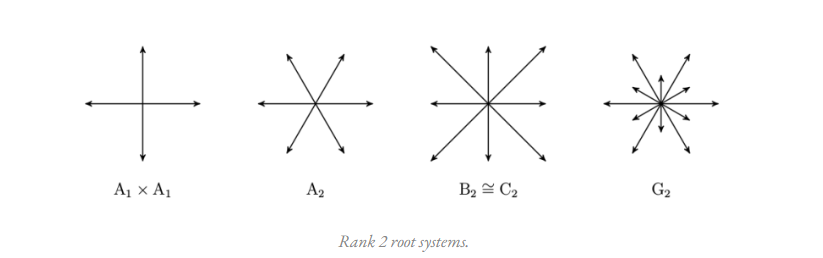
\includegraphics[scale=0.5]{chapters/rank2rootsystems.png}
        \end{center}
    \end{lemma}
\end{dang}
Proof: We prove it in several steps:
\begin{itemize}
    \item Claim: Every two adjacent roots have the same angle between then. \par 
    Let $\alpha_0,\alpha_1\in\Delta$ be two adjacent roots with minimum angle between then. We define 
    \begin{equation}
        \alpha_{n+1}=-r_{\alpha_n}(\alpha_{n-1})\in\Delta,\;n\geq1
    \end{equation}
    and $\text{Arg}(v)=\cos^{-1}(\frac{(v,\alpha_0)}{\|v\|\|\alpha_0\|})\in [0,2\pi)$.
With this definition, we see that the angle between $\alpha_n$ and $\alpha_{n-1}$ for $n\geq1$ still $\theta$. 
In fact 
\begin{equation}
    \begin{split}
        \frac{(\alpha_n,\alpha_{n-1})}{\|\alpha_n\|\|\alpha_{n-1}\|}&=
        \frac{(r_{\alpha_{n-1}}(\alpha_{n-2}),\alpha_{n-1})}{\|r_{\alpha_{n-1}}(\alpha_{n-2})\|\|\alpha_{n-1}\|}\\
        &=\frac{(\alpha_{n-2},\alpha_{n-1})}{\|\alpha_{n-2}\|\|\alpha_{n-1}\|}
        \;(r_{\alpha_{n-1}}\text{ is an isometry})\\
        &\cdots\\
        &=\frac{(\alpha_1,\alpha_0)}{\|\alpha_1\|\|\alpha_0\|}.
    \end{split}
\end{equation}
    In this condition we claim that we have $\text{Arg}(\alpha_n)=n\theta\text{ mod }2\pi$,
    where $\theta=\text{Arg}(\alpha_1)$.
    We argue by induction, the base case being
    just the definition. The induction step follows by the calculation
    \begin{equation}
        \begin{split}
            \cos \text{Arg}(\alpha_{n+1})&=\frac{( \alpha_{n+1}, \alpha_0 )}{\| \alpha_{n+1} \|} \\
        &= 2 \frac{( \alpha_{n-1}, \alpha_n )}{\| \alpha_n \| \| \alpha_{n-1} \|} 
        \cdot \frac{( \alpha_n, \alpha_0 )}{\| \alpha_n \|}- \frac{( \alpha_{n-1},\alpha_0 )}{\| \alpha_{n-1} \|} \\
        &= 2 \cos(\theta) \cos(n\theta) - \cos((n-1)\theta) \\
        &= \cos((n+1)\theta).
        \end{split}
    \end{equation}
   Now let $n=\text{Max}\{k\geq1:n\theta\leq2\pi\}$. If $n\theta<2\pi$, then $2\pi <(n+1)\theta<\theta + 2\pi$, which 
   is a contradiction with the hipothesis that $\theta$ is the smallest angle between two adjacent roots. Therefore, we 
   see that $n\theta=2\pi$ and $\theta=2\pi/n$. Since the only colinear roots are $\{\pm\alpha\}$, we see that we have 
   obtained all roots by this process, because of the condition of minimality of $\theta$.
   
   \item Remember that if $\alpha,\beta\in\Delta$, then 
   \begin{equation}
    2\frac{(\alpha,\beta)}{(\alpha,\alpha)}\in\mathbb{Z}.
   \end{equation}
   Therefore, if $\alpha,\beta$ are two adjacent roots we get 
   \begin{equation}
    4\cos^2(\theta)=4\frac{(\alpha,\beta)}{(\alpha,\alpha)(\beta,\beta)} \in\{0,1,2,3,4\} 
\text{ (apply Cauchy-Scharwz)}.
   \end{equation}
So, we have $|\cos(\theta)|\in\{0,\frac12,\frac{1}{\sqrt{2}},\frac{\sqrt{3}}{2},1\}$ and 
$\theta\in\{\frac{\pi}{2},\frac{\pi}{3},\frac{\pi}{4},\frac{\pi}{6}\}$. Here 0 is excluded because $\beta\neq\alpha$.
The next step is to describe the roots system, i.e., find explictly all elements of $\Delta$ for each angle 
$\theta$ obtained. Before we proceed, we have a observation: Each $\theta$ is of the form $\pi/n$ and we saw in the previous item 
that $\text{Arg}(\Delta)=\{\frac{k\pi}{n}:k=0,\dots,2n-1\}$, so $\#\Delta=2n$. 


\item Case $n=4$: In this case we have 8 roots. Lets find them in polar coordinates using complex number notation.
Suppose that $\alpha,\beta\in \Delta\subset\bbC$ are two adjacent roots. 
We can assume $\text{Arg}(\alpha)=0$ and $\text{Arg}(\beta)>0$ (this condition will be used in all the cases).\par 

We have
\begin{equation}
    4\cos^2(\theta)=2\frac{(\alpha,\beta)}{(\alpha,\alpha)}\cdot 2\frac{(\alpha,\beta)}{(\beta,\beta)}=2
\end{equation}
and without lost of generality we assume that 
\begin{equation}
    2\frac{(\alpha,\beta)}{(\alpha,\alpha)}=2,\;2\frac{(\alpha,\beta)}{(\beta,\beta)}=1\Rightarrow 
    \frac{(\beta,\beta)}{(\alpha,\alpha)}=2.
\end{equation}
So we can assume $(\beta,\beta)=2,\;(\alpha,\alpha)=1$, which implies $\alpha=1$ and $\beta=\sqrt{2}\exp(\frac{i\pi}{4})$.
Now, since $2\frac{(\alpha,\beta)}{(\alpha,\alpha)}=2$, we see that $\beta-2\alpha\in\Delta$, i.e., 
$\sqrt{2}\exp(\frac{3i\pi}{4})\in\Delta$. Furthermore $2\frac{(\alpha,\beta)}{(\beta,\beta)}=1$ implies that 
$\alpha-\beta=-i\in\Delta$. Then the four roots in the upper plane are 
\begin{equation}
    1, \sqrt{2}\exp(\frac{i\pi}{4}), i\;\text{ and }\sqrt{2}\exp(\frac{3i\pi}{4}).
\end{equation}
These roots determines all the 8 roots of $\Delta$.

\item Case $n=3$: In this case we have 6 roots. We have 
\begin{equation}
    4\cos^2(\theta)=2\frac{(\alpha,\beta)}{(\alpha,\alpha)}\cdot 2\frac{(\alpha,\beta)}{(\beta,\beta)}=2
\end{equation}
and we can assume 
\begin{equation}
    2\frac{(\alpha,\beta)}{(\alpha,\alpha)}=1,\; 2\frac{(\alpha,\beta)}{(\beta,\beta)}=1.
\end{equation}
So $(\alpha,\alpha)=(\beta,\beta)=1$, which implies $\alpha=1$ and $\beta=\exp(\frac{i\pi}{3})$. Now, since 
$2\frac{(\alpha,\beta)}{(\alpha,\alpha)}=1$, we have $\beta-\alpha=\exp(\frac{2i\pi}{3})\in\Delta$. From this we get 
all the 3 roots in the upper plane. This determines all the other roots in $\Delta$:
\begin{equation}
    \exp(\frac{ki\pi}{3}),\;k=0,1,2,3,4,5.
\end{equation}

\item Case $n=2$: In this case we have 4 roots. We have 
\begin{equation}
    4\cos^2(\theta)=2\frac{(\alpha,\beta)}{(\alpha,\alpha)}\cdot 2\frac{(\alpha,\beta)}{(\beta,\beta)}=0
\end{equation}
and we can assume 
\begin{equation}
    2\frac{(\alpha,\beta)}{(\alpha,\alpha)}=0\Rightarrow (\alpha,\beta)=0.
\end{equation}
So $\alpha=1$ and $\beta = mi,m\geq0$ and it remains to find $m$.

\item Case $n=6$: In this case we have 12 roots. Lets find them. We have 
\begin{equation}
    4\cos^2(\theta)=2\frac{(\alpha,\beta)}{(\alpha,\alpha)}\cdot 2\frac{(\alpha,\beta)}{(\beta,\beta)}=3
\end{equation}
and we can assume 
\begin{equation}
    2\frac{(\alpha,\beta)}{(\alpha,\alpha)}=1,\;2\frac{(\alpha,\beta)}{(\beta,\beta)}=3
\end{equation}
so we take $(\alpha,\alpha)=3(\beta,\beta)=3$. Then if $\alpha=\sqrt{3}$, we get $\beta =\exp(\frac{i\pi}{6})$. 
Now, condition $2\frac{(\alpha,\beta)}{(\alpha,\alpha)}=1$ implies that $\beta-\alpha = \exp(\frac{5i\pi}{6})\in\Delta$. 
Moreover, condition $2\frac{(\alpha,\beta)}{(\beta,\beta)}=3$ implies that 
\begin{equation}
    \begin{split}
        &\alpha-2\beta= -i \in\Delta\\
        &\alpha-3\beta=\sqrt{3}\exp(\frac{4i\pi}{3})\in\Delta
    \end{split}
\end{equation}
This determines all the 6 root in the upper half plane and therefore, all the other roots in $\Delta$.
\end{itemize}

We could have used the previous algorithm to construct all roots in each case: For the initial adjacent roots 
$\alpha_0,\alpha_1$, all other roots are of the form $\alpha_{n+1}=-r_{\alpha_n}(\alpha_{n-1}),\;n\geq1$. For
example, in the case $n=4$ we have $\alpha_0=1$ and $\alpha_1=\sqrt{2}\exp(\frac{i\pi}{4})$. Then 
\begin{equation}
    \begin{split}
        \alpha_2&=-1+\text{Re}(1\cdot\overline{\sqrt{2}\exp(\frac{i\pi}{4})})\sqrt{2}\exp(\frac{i\pi}{4})\\
    &=-1+2\frac{1}{\sqrt{2}}\exp(\frac{i\pi}{4})\\
    &=i
    \end{split} 
\end{equation}
and 
\begin{equation}
    \begin{split}
        \alpha_3&=-\sqrt{2}\exp(\frac{i\pi}{4})+2\text{Re}[(-i)\sqrt{2}\exp(\frac{i\pi}{4})]i\\
    &=-\sqrt{2}\exp(\frac{i\pi}{4})-2i\\
    &=-1-i\\
    &=\sqrt{2}\exp(\frac{3i\pi}{4}).
    \end{split}
\end{equation}

\begin{dang}
    \begin{example}
        The Lie algebra $\fr{so}_8$ has root system given by:
        \begin{equation}
            \Delta=\{L_i-L_j:i\neq j\}\cup\{\pm(L_i+L_j):i\neq j\}
        \end{equation}
        for $i,j\in\{1,2,3,4\}$. Let $f:\text{Span}(L_i)_{1\leq i\leq4}\to\mathbb{R}$ be a linear map such that 
        $f(L_1)>f(L_2)>f(L_3)>f(L_4)>0$. Then, with respect to this linear functional we get 
        \begin{equation}
            \Delta_+=\{L_i-L_j:i>j\}\cup\{L_i+L_j:i\neq j\}
        \end{equation}
        and $\Pi=\{L_1-L_2,L_2-L_3,L_3-L_4,L_3+L_4\}$. 
    \end{example}
\end{dang}
It's a interesting exercise to decompose $\fr{so}_8$ as a sum of $\fr{sl}_2$-modules with respect to the adjoint action 
of the positive element $X_{\alpha},\;\alpha=L_1-L_2$. To do this, we list the corresponding strings of $\fr{sl}_2-$modules.
The arrows ``$\to$'' corresponds to the action of $\ad(X_{\alpha})$ on the respective root spaces.
\begin{equation}
    \begin{split}
        &-L_1+L_2\to H_{L_1-L_2}\to L_1-L_2 \to 0 \Rightarrow V_{(2)}\;(\text{because }(\alpha,L_1-L_2)=2)\\
        &L_2-L_3 \to  L_1-L_3\to0\Rightarrow V_{(1)}\;(\text{because }(\alpha,L_1-L_3)=1)\\
        &L_2-L_4\to L_1-L_4\to 0\Rightarrow V_{(1)}\;(\text{because }(\alpha,L_1-L_4)=1)\\
        &L_3-L_4\to 0\Rightarrow V_{(0)}\;(\text{because }(\alpha,L_3-L_4)=0)\\
        &L_1+L_2\to 0\Rightarrow V_{(0)}\;(\text{because }(\alpha,L_1+L_2)=0)\\
        &L_2+L_3\to L_1+L_3\to0\Rightarrow V_{(1)}\;(\text{because }(\alpha,L_1+L_3)=1)\\
        &L_2+L_4\to L_1+L_4\to0\Rightarrow V_{(1)}\;(\text{because }(\alpha,L_1+L_4)=1)\\
        &L_3+L_4\to0\Rightarrow V_{(0)}\;(\text{because }(\alpha,L_3+L_4)=0)
    \end{split}
\end{equation}
So the positive root spaces gives a contribution 
$V_{(2)}\oplus V_{(1)}^{\oplus 4}\oplus V_{(0)}^{\oplus 3}$ to the decomposition
of $\fr{so}_2$ into $\fr{sl}_2-$modules. Also, there is only one element $H_\alpha$ of the Cartan subalgebra $\fr{h}$ in this decomposition.
So it remais to determine the decomposition of $\bigoplus_{\alpha\in\Delta_+}\fr{g}_{-\alpha}$ and the rest of the Cartan 
subalgebra. However, we can see by the same reasoning that 
\begin{equation}
    \bigoplus_{\alpha\in\Delta_+}\fr{g}_{-\alpha}\cong V_{(2)}\oplus V_{(1)}^{\oplus 4}\oplus V_{(0)}^{\oplus 3}
\end{equation}
and since $\fr{h}=\bbC H_\alpha\oplus\Ker(\alpha)$, we get the contribution of the remaining elements of the Cartan subalgebra:
\begin{equation}
    \Ker(\alpha)\cong V_{(0)}^{\oplus 3}\;(\text{because }\dim(\fr{h})=4).
\end{equation}
So, the final result is $\fr{g}\cong V_{(2)}\oplus V_{(1)}^{\oplus 8}\oplus V_{(0)}^{\oplus 9}$. As a test, we sum the 
corresponding dimensions:
\begin{equation}
    \dim(V_{(2)}\oplus V_{(1)}^{\oplus 8}\oplus V_{(0)}^{\oplus 9})=3+8\cdot 2+9\cdot 1=3+16+9=28.
\end{equation}
Which confirms the calculation $\dim(\fr{so}_8)=2\cdot 4^2-4=28$.


\section{Simple Lie algebras}
\subsection{Irreducible root systems}
\begin{dang}
    \begin{definition}
        A root system $(V,\Delta)$ is sai do to be decomposable if there exist a decomposition $V=V_1\oplus V_2$
        such that $\Delta=(\Delta\cap V_1)\cup (\Delta\cap V_2)$. An irreducible root system, is a root system 
        that is not decomposable.
    \end{definition}
\end{dang}

\begin{dang}
    \begin{lemma}
        If $(V,\Delta)$ is decomposable with $\Delta=\Delta_1\cup\Delta_2,\;\Delta_i\subset V_i, V=V_1\oplus V_2$, 
        then $V_1\perp V_2$.
    \end{lemma}
\end{dang}
Proof: Suppose that $\alpha\in \Delta_1,\beta\in \Delta_2$ and $(\alpha,\beta)\neq0$. Since 
\begin{equation}
    p-q=2\frac{(\alpha,\beta)}{(\alpha,\alpha)}\neq0
\end{equation}
we have two cases:
\begin{itemize}
    \item If $p >q$, then $p\geq1$ and $\beta-\alpha\in \Delta$. But this can not happen, because if 
    $\beta-\alpha\in\Delta_1\overset{\alpha\in V_1}{\Rightarrow}\beta\in \Delta\cap V_1=\Delta_1$. 
    In a similar way we see that we 
    can not have $\beta-\alpha\in\Delta_2$.
    \item If $q>p$, then $\beta+\alpha\in\Delta$ an the exact same reasoning apply to show that this let to a contradiction.
\end{itemize}
\qed

\begin{dang}
    \begin{remark}
        Since $\Delta$ contain a basis of $V$ it can not be the case that $\Delta$ is contained in a proper subspace of $V$. 
        So, if $V=V_1\oplus V_2$ is a nontrivial decomposition, we must have $\Delta_i=\Delta\cap V_i\neq\varnothing$. 
    \end{remark}
\end{dang}

\begin{dang}
    \begin{remark}
        Maybe we can show that $(V_i,\Delta_i)$ are root systems, but we will not need it.
    \end{remark}
\end{dang}


\begin{dang}
    \begin{theorem}
        Let $\fr{g}$ be a Lie algebra with associated root system $(\fr{h}^*,\Delta)$ where $\fr{h}$ is a 
        Cartan subalgebra. Then 
        \begin{equation}
            \fr{g} \text{ is simple }\iff (\fr{h}^*,\Delta)\text{ is irreducible}.
        \end{equation}
    \end{theorem}
\end{dang}
Proof:($\Leftarrow$). Suppose that $\fr{g}=\fr{g}_1\oplus\fr{g}_2$ with $\fr{g}_i$ semisimple with a choice of Cartan subalgebras
$\fr{h}_i\;(i=1,2)$. Then, we see that $\fr{h}=\fr{h}_1\oplus\fr{h}_2\subset \fr{g}$ is Cartan. In fact, since 
$[\fr{h}_1,\fr{h}_2]=0$ we see that $\fr{h}^k=\fr{h}_1^k\oplus\fr{h}_2^k$, so $\fr{h}$ is nilpotentl. Moreover 
\begin{equation}
    \begin{split}
        &[(X,Y),\fr{h}_1\oplus\fr{h}_2]\subset \fr{h}_1\oplus\fr{h}_2\iff\\
        &([X,\fr{h}_1],[(Y,\fr{h}_2)])\subset \fr{h}_1\oplus\fr{h}_2\iff\\
        &[X,\fr{h}_i]\subset \fr{h}_i\;(i=1,2).
    \end{split}
\end{equation}
Then $X\in N(\fr{h}_1)=\fr{h}_1$ and $Y\in N(\fr{h}_2)=\fr{h}_2$, so $(X,Y)\in\fr{h}$. In particular this shows that 
\begin{equation}
    \text{Rank}(\fr{g}_1\oplus\fr{g}_2)=\text{Rank}(\fr{g}_1)+\text{Rank}(\fr{g}_2).
\end{equation}
Now identify $\fr{h}^*=\fr{h}_1^*\oplus\fr{h}_2^*$ with the rule 
$(\alpha,\beta)(v,w)=\alpha(v)+\beta(w)$. Then we claim that if $\alpha\in\Delta_1$, then $(\alpha,0)\in\Delta$. In fact, 
for $v\in\fr{g}_\alpha\setminus0$, we have  
\begin{equation}
    \begin{split}
        [(H_1,H_2),(v,0)]&=([H_1,v],0)\\
        &=(\alpha(H_1)v,0)\\
        &=\alpha(H_1)(v,0)\\
        &=(\alpha,0)(H_1,H_2)\cdot(v,0).
    \end{split}
\end{equation}
So $\fr{g}_{(\alpha,0)}\neq0$ and $(\alpha,0)\in\Delta$. In a similar way we show that $(0,\beta)\in\Delta$ for 
$\beta\in\Delta_2$. Therefore 
\begin{equation}
    (\Delta_1\times 0) \cup (0\times\Delta_2)\subset \Delta.
\end{equation}
Conversely, if $(\alpha,\beta)\in\Delta$, then there exist $(v,w)\in\fr{g}_{(\alpha,\beta)}\setminus0$. So
\begin{equation}
    \begin{split}
       ([H_1,v],[H_2,w]) =[(H_1,H_2),(v,w)]=(\alpha(H_1)+\beta(H_2))\cdot(v,w),\;\forall (H_1,H_2)\in\fr{h}_1\oplus\fr{h}_2.
    \end{split}
\end{equation}
If $v\neq0$, then taking by taking $H_1=0$ on the previous equation we see that 
\begin{equation}
    (0,[H_2,w])=\beta(H_2)\cdot(v,w)
\end{equation}
and $\beta(H_2)v = 0\Rightarrow \beta(H_2)=0,\;\forall H_2\in\fr{h}_2$. Therefore $\beta=0$ and by applying 
the same reasoning for $H_2=0$ we will conclude that $\alpha\in\Delta_1$ while $w=0$. So this proves the other inclusion.\par 

$(\Rightarrow)$. Suppose that $(\fr{h}^*,\Delta)$ is decomposable, so there exist decomposition 
\begin{equation}
    \fr{h}^*=\fr{h}_1^*\oplus\fr{h}_2^*,\;\Delta_i=\Delta\cap\fr{h}_i^*, \Delta=\Delta_1\cup\Delta_2.
\end{equation}
In this condition, we claim that $\fr{g}_1=\bigoplus_{\alpha\in\Delta_1}\fr{g}_\alpha$ is a proper ideal 
in $\fr{g}$. In fact, we see that $\fr{g}_\beta,\;\beta\in\Delta_2$ is not contained in $\fr{g}_1$. Now, it's clear 
that $\fr{g}_1$ is invariant by the adjoint action of $X_\alpha,\;\alpha\in\Delta_1$. It also happens that it is 
invariant by the adjoint action of $X_\beta,\;\beta\in\Delta_2$. In fact if $[X_\beta, X_\alpha]\neq0$ for $\alpha\in\Delta_1$ and 
$\beta\in\Delta_2$, then 
\begin{equation}
    \alpha+\beta\in\Delta
\end{equation}
which can not happen, as we saw before.\qed

\begin{dang}
    \begin{lemma}\label{Lemma: criteria to irreducible root systems}
        We have a nice criterion to find irreducible root systems $(V,\Delta)$. In fact, if for any 
        $\alpha,\beta\in\Delta$ we have a sequence $\gamma_0,\gamma_1,\dots,\gamma_{n+1}$ such that 
        \begin{itemize}
            \item $\gamma_0=\alpha$ and $\gamma_{n+1}=\beta$
            \item $\gamma_i+\gamma_{i+1}\in\Delta$
        \end{itemize}
        then $\Delta$ is irreducible.
    \end{lemma}
\end{dang}
Proof: To show this, assume that $V=V_1\oplus V_2$ and $\Delta=\Delta_1\cup\Delta_2,\;\Delta_i=V_i\cap \Delta$.
Let $\alpha\in\Delta_1, \beta\in\Delta_2$ and $(\gamma_i)_0^{n+1}$ a sequence of roots satisfying the condition of 
the lemma. Then we see that $\alpha+\gamma_1\in\Delta\overset{\alpha\in V_1}{\Rightarrow}\gamma_1\in \Delta_1$. 
So, proceding by induction and using the condition $\gamma_i+\gamma_{i+1}\in\Delta$ we will conclude that 
$\gamma_i\in\Delta_1,\;\forall i$. In particular, this we have $\beta=\gamma_{n+1}\in\Delta_1$, which is a contradiction.
\qed

\subsection{Root systems of simple Lie algebras}
An useful about invariant forms on simple Lie algebras.
\begin{dang}
    \begin{lemma}
        Any invariant bilinear form $(\cdot,\cdot)$ on a simple Lie algebra is symmetric.
    \end{lemma}
\end{dang}
Proof: Observe that for all $X,Y,Z\in\fr{g}$ we have 
\begin{equation}
    \begin{split}
        ([X,Y],Z)&=(X,[Y,Z])\\
        &=-(X,[Z,Y])\\
        &=-([X,Z],Y)\\
        &=([Z,X],Y)\\
        &=(Z,[X,Y]).
    \end{split}
\end{equation}
Since a simple Lie algebra is perfect, i.e., $[\fr{g},\fr{g}]=\fr{g}$, we are done.\qed



\begin{dang}
    \begin{lemma}
        Let $\fr{g}\subset\End(V)$ be a simple Lie algebra. 
        Then any invariant form will be a multiple of the trace form:
        \begin{equation}
            (X,Y)=\Tr(XY).
        \end{equation}
    \end{lemma}
\end{dang}
Proof: We prove that the vector space of invariant bilienar forms is 1. Let $(\cdot,\cdot)_i,\;i=1,2$ two invariant forms and 
define $\nu:\fr{g}\overset{\cong}{\to}\fr{g}^*:X\mapsto (X,\cdot)_1$. Then, for any $X\in \fr{g}$, we define $M(X)=\nu^{-1}(X,\cdot\;)_2$. It's clear 
that $M\in\End(\fr{g})$. We have more: $M$ is lie algebra morphism $\fr{g}\to \fr{g}$. In fact for any $X,Y,Z\in\fr{g}$ we have
\begin{equation}
    \begin{split}
        (M[X,Y],Z)_1&=([X,Y],Z)_2\;(\text{definition of }M)\\
        &=(X,[Y,Z])_2\;(\text{invariance of }(\cdot,\cdot)_2)\\
        &=(Mx,[Y,Z])_1\;(\text{definition of }M)\\
        &=([Mx,Y],Z)_1\;(\text{invariance of }(\cdot,\cdot)_1).
    \end{split}
\end{equation}  
So, by nondegeneracy of $(\cdot,\cdot)_1$ we have $M[X,Y]=[Mx,Y]$, i.e., $M\circ \ad(X)=\ad\circ M(X)$ and $M$ is a intertwining 
operator $\fr{g}\to\fr{g}$ relative to the adjoint action of $\fr{g}$ on itself. Therefeore $M=c\mathds{1}_{\fr{g}}$ by the Schur's Lemma. 
This means that $c(\cdot,\cdot)_1=(\cdot,\cdot)_2$.\par 
Finally, since the trace form is an invariant bilinear form, we get the result.\qed

Next, we will compute the dimension, rank and the Cartan matrix of some simple classical Lie algebras.

\subsubsection{\texorpdfstring{Family $A_n$:}{Family \text{An}:}}
This family corresponds to the Lie algebras $\fr{sl}_{n},\;n\geq1$. 
First, we prove that $\fr{sl}_n$ is a semisimple Lie algebra. We will use lemma~(\ref{Lemma: alternative criteria for ss Lie algebras}). 
Since $I_V\notin\fr{sl}_n$ we need to show that its tautological representation is irreducible. Let $W\subset V=\bbR^n$ be a 
nonzero invariant subspace and let $w\in W\setminus0$. Write $w=(a_1,\dots,a_n)$ and let $j$ be such that $a_j\neq0$. Then 
$E_{1j}(w)=a_je_1\in W\Rightarrow e_1\in W$. We continue in this way by applying $E_{21},E_{32},\dots, E_{n,n-1}$ to conclude that 
$e_1,\dots, e_n\in W$, so $W=V$. Now, we apply lemma~(\ref{Lemma: Criteria to find Cartan subalgebras}) to conclude that 
$\fr{h}=\{\text{Diag}(\lambda_1,\dots,\lambda_n):\sum_j\lambda_j=0\}$ is a Cartan subalgebra of $\fr{sl}_n$. From this we see that 
$E_{ij}\subset\fr{g}_{L_i-L_j},\;i\neq j$ and since the weight spaces are one dimensional we get $\fr{g}_{L_i-L_j}=\bbC E_{ij}$. So we 
get the weightspace decomposition of $\fr{sl}_n$:
\begin{equation}
    \fr{sl}_n = \fr{h}\oplus\bigoplus_{i\neq j}\fr{g}_{L_i-L_j},\;\fr{g}_{L_i-L_j}=\bbC E_{ij},\; \fr{h}=\{\text{Diag}(\lambda_1,\dots,\lambda_n):\sum_j\lambda_j=0\}.
\end{equation}
So, the root system associated to $\fr{sl}_n$ is:
\begin{equation}
    \Delta=\{L_i-L_j:i\neq j,\; 1\leq i,j\leq n\}\subset \text{Span}(L_i)_{i=1}^n\cong\bbR^n.
\end{equation}
Note that $\Delta$ lies in the subspace $\{a_1L_1+\cdots+a_nL_n:\sum_ja_j=0\}$. Now,
the choice of linear functional $f: L_i\mapsto n-i+1$ yields positive roots:
\begin{equation}
\Delta_+=\{L_i-L_j:i<j,\;1\leq i,j\leq n\}.    
\end{equation}
The simple roots are $\Pi=\{\alpha_1,\dots,\alpha_{n-1}\},\;\alpha_i=L_i-L_{i+1}$. So far we got:
\begin{dang}
    \begin{equation}
    \dim(\fr{sl}_n)=n^2-1,\;\text{Rank}(\fr{sl}_n)=n-1,\;\#\Delta = n(n-1).
\end{equation}
\end{dang}
Now we need to compute the Cartan matrix of $\fr{sl}_n$. Recall that 
if $\alpha,\beta\in\fr{h}^*$, then 
\begin{equation}
    \beta(H_\alpha)=\frac{2}{(\alpha,\alpha)}\beta(\nu^{-1}(\alpha))=2\frac{(\alpha,\beta)}{(\alpha,\alpha)}.
\end{equation}
So the Cartan matrix can be expressed by $(\alpha_j(H_{\alpha_i}))_{i,j=1}^{n-1}$. Furthermore, we know that if
$(Y,X)\in\fr{g}_{-\alpha}\times\fr{g}_\alpha$, then $[X,Y]=K(X,Y)\nu^{-1}(\alpha)$. Now, define $H=[X,Y]$ and suppose that 
$[H,X]=2X$. Then $\alpha(H)=K(X,Y)(\alpha,\alpha)=2$, i.e., $H=[X,Y]=H_\alpha$. This shows that 
$H_{i,j}=[E_{ij}, E_{ji}]=\text{Diag}(0,\dots,0,\hat{1},\dots,-\hat{\hat{1}},0,\dots,0),\;(\;\hat{}=i\text{th},\hat{\hat{}}=j\text{th position})$ is 
 the coroot relative to $L_i-L_j$, i.e., $H_{i,j}=H_{L_i-L_j},\;i<j$.\par

 Now define the form $(L_i,L_j)=\delta_{ij}$. Then we see that, with respect to this form we have 
 \begin{equation}
    2\frac{(\alpha_i,\alpha_j)}{(\alpha_i,\alpha_i)}=\left\{\begin{aligned}
        &-1\;\text{ if }|i-j|=1\\
        &\;\;0\;\text{ if }|i-j|>1\\
        &\;\;2\;\text{ if }i=j.
    \end{aligned}\right.
 \end{equation}
 This agrees with the values $\alpha_j(H_{\alpha_i})$, so this orthonormal form must be a multiple of the Killing form transposed to 
 $\fr{h}^*$.\par 

 Finally we show that $\fr{sl}_n$ is in fact a simple Lie algebra. 
 To do this we use lemma~(\ref{Lemma: criteria to irreducible root systems}): observe that if $\alpha=L_i-L_j, \beta=L_k-L_l\;(i<j<k<l)$, then 
 we take 
 \begin{equation}
    \alpha=\gamma_0=L_i-L_j,\;  \gamma_1=L_j-L_k    ,\;\beta=\gamma_2 = L_k-L_l.
 \end{equation}

\subsubsection{\texorpdfstring{Family $C_n$:}{Family \text{Cn}:}}
This family corresponds to the simplectic Lie algebra $\fr{sp}_{2n}$ defined by 
\begin{equation}
    \fr{sp}_{2n}=\{X\in M_{2n}(\bbC): X^T\Omega+\Omega X=0\},\;\Omega = \begin{pmatrix}
        0& I_n\\ -I_n&0
    \end{pmatrix}\in M_{2n}(\bbC).
\end{equation}
More explictly: $\fr{sp}_{2n}=\left\{\begin{pmatrix}A&B\\C&-A^T\end{pmatrix}: B=B^T,C=C^T\right\}$.
\begin{itemize}
    \item We claim that $\fr{sp}_{2n}$ is semisimple. To show this we use lemma~(\ref{Lemma: alternative criteria for ss Lie algebras}). 
    Since $I_{2n}\notin\fr{sp}_{2n}$ we only need to show that the tautological representation is irreducible. Observe that
    $E_{j,n+j},E_{n+j,k},E_{ij}-E_{n+j,n+i}\in\fr{sp}_{2n},\;(1\leq i,j\leq n)$. If $W\subset V$ is a nonzero invariant subspace, then 
    there exist $w=(a_1,\dots,a_{2n})^T\in W\setminus0$. Without lost of generalization we can assume that $a_k\neq0$ for some 
    $k,\;(1\leq k\leq n)$. If this is not the case, then there exist $a_{n+k}\neq0$ for some $k,\;(1\leq k\leq n)$ and we apply 
    $E_{k,n+k}w=a_{n+k}e_k\in W$. Now, with the assumption that $a_k\neq0$ we apply $E_{k,n+k}E_{n+k,k}w=a_ke_k\in W$ to conclude that 
    $e_k\in W$. Finally, we can use the elements $E_{ik}-E_{n+k,n+i},\;i=1,\dots, n$ to conclude that $e_1,\dots, e_n\in W$ and again 
    we use $E_{n+i,i}$ to conclude that $e_{n+1},\dots, e_{2n}\in W$. So $W=V$ and $\fr{sp}_{2n}$ is semisimple. 
    \item Since we know that $\fr{sp}_{2n}$ is semisimple, we use the fact that 
    \begin{equation}
        \text{Diag}(\lambda_1,\dots,\lambda_n,-\lambda_1,\dots,-\lambda_n)\in\fr{sp}_{2n}\text{ for }\lambda_i\neq\lambda_j
    \end{equation}
   to conclude that its diagonal elements forms a Cartan subalgebra 
    \begin{equation}
        \fr{h}=\left\{\text{Diag}(\lambda_1,\dots,\lambda_n,-\lambda_1,\dots,-\lambda_n) : \lambda_i\in\bbC,\;i=1,\dots,n \right\}.
    \end{equation}
\begin{dang}
    \begin{remark}
        In the following, we will identify $\fr{h}\cong \{\text{Diag}(\lambda_1,\dots,\lambda_n):\lambda_i\in\bbC\}$. So we will 
        construct its weight space decomposition using linear functionals $L_i,\;i=1,\dots,n$. In fact we have the identification
        \begin{equation}
            L_{n+i}+L_i =0
        \end{equation}
        on $\fr{h}$.
    \end{remark}
\end{dang}

    The corresponding weight space decomposition is the following:
    \begin{equation}
        \begin{aligned}
            &Y_{ij}=E_{i,n+j}+E_{j,n+i}\;(1\leq i\leq j\leq n)\\
            &X_{ij}=E_{ij}-E_{n+j,n+i}\;(1\leq i,j\leq n, i\neq j) \\
            &Z_{ij}=E_{n+i,j}+E_{n+j,i}\;(1\leq i\leq j\leq n).
        \end{aligned}
    \end{equation}

To find the corresponding weights we compute 
\begin{equation}
    \begin{aligned}
        &[H,Y_{ij}]=(\lambda_i+\lambda_j)E_{i,n+j}+(\lambda_j+\lambda_i)E_{j,n+i}=(L_i+L_j)(H)Y_{ij}\\
        &[H,X_{ij}]=(\lambda_i-\lambda_j)E_{ij}-(-\lambda_j+\lambda_i)E_{n+j,n+i}=(L_i-L_j)(H)X_{ij}\\
        &[H,Z_{ij}]=(-\lambda_i-\lambda_j)E_{n+i,j}+(-\lambda_j-\lambda_i)E_{n+j,i}=-(L_i+L_j)(H)Z_{ij}.
    \end{aligned}
\end{equation}
So 
\begin{equation}
    \Delta = \{L_i-L_j:i\neq j\}\cup \{\pm(L_i+L_j): i\leq j\},\; i,j\in\{1,\dots,n\}.
\end{equation}
The choice of linear functional $f:\fr{h}^*\to\bbR$ such that $f(L_1)>\cdots >f(L_n)>0$ yields positive roots given by 
\begin{equation}
    \Delta_+=\{L_i-L_j: i< j\}\cup \{L_i+L_j : i\leq j\}.
\end{equation}
By excluding roots which are um of other positive roots we get the set of simple roots 
\begin{equation}
    \Pi=\{L_1-L_2,\dots, L_{n-1}-L_n, 2L_n\}. 
\end{equation}
We will write $\alpha_i=L_i-L_{i+1},i=1,\dots,n-1$ and $\alpha_n=2L_n$ to the simple roots. So far we got 
\begin{dang}
    \begin{equation}
        \dim(\fr{sp}_{2n})=2n^2+n,\;\text{Rank}(\fr{sp}_{2n})=n,\;\#\Delta = 2n^2.
    \end{equation}
\end{dang}
\item Now we compute the Cartan matrix of $\fr{sp}_{2n}$. To do this we use the same approach made in the case $A_n$.
Remember that $\bbC Y_{ij}=\fr{g}_{L_i+L_j}, \bbC X_{ij}=\fr{g}_{L_i-L_j}$ and $\bbC Z_{ij}=\fr{g}_{-(L_i+L_j)}$. So we find
the coroots:
\begin{equation}
    \begin{aligned}
        &[Y_{ij},Z_{ij}]=H_{i,n+j}+H_{j,n+i}=H_{L_i+L_j},\;i\neq j \\
        &[Y_{ii}/2,Z_{ii}/2]=H_{i,n+i}=H_{2L_i}\\
        &[X_{ij},X_{ji}]=H_{i,j}+H_{n+j,n+i}=H_{L_i-L_j},\;i<j.
    \end{aligned}
\end{equation}
Now we get 
\begin{equation}
   \alpha_j(H_{\alpha_i})=\left\{\begin{aligned}
    & 2\;\text{ if } i=j\\
    & 0\;\text{ if } |i-j|>1\\        
    & -1\;\text{ if } |i-j|=1
    \end{aligned}\right.\; (1\leq i,j\leq n)
\end{equation}
and 
\begin{equation}
    \alpha_n(H_{\alpha_i})=\left\{\begin{aligned}
        & 0 \;\text{ if } i<n-1\\
        &-2\;\text{ if } i=n-1
    \end{aligned}\right.,\;
    \alpha_i(H_{\alpha_n})=\left\{\begin{aligned}
        & 0 \;\text{ if } i<n-1\\
        &-1\;\text{ if } i=n-1
    \end{aligned}\right.\;(1\leq i\leq n)
\end{equation}
So, the Cartan matrix of $\fr{sp}_{2n}$ is compatible with the form $(L_i,L_j)=\delta_{ij}$. Furthermore, its 
associated Dynkin diagram is: 
\[
\xymatrix{
    \underset{1}{\circ}\ar@{-}[r]&\underset{2}{\circ}\ar@{-}[r]&
    \cdots\ar@{-}[r]&\underset{n-1}{\circ}\ar@{-}[r]<0.2ex>\ar@{-}[r]<-0.2ex>&\underset{n}{\circ}
}
\]
which is connected, so $\fr{sp}_{2n}$ is simple.
\end{itemize}

\subsubsection{\texorpdfstring{Family $D_n$:}{Family \text{Dn}:}}
This family corresponds to the Lie algebra $\fr{so}_{2n}$. It's usual presentation is as the set of matrices $X$ satisfying 
$X^T+X=0$ (skew symmetric matrices). However, this presentation is not useful (to us), because we can not use the 
lemma~(\ref{Lemma: Criteria to find Cartan subalgebras}) to decribe its Cartan subalgebras.\par 

In general, let $(q,V)$ be a quadratic space, i.e., $V$ is a vector space and $q:V\to\mathbb{F}$ is a quadratic form. So, by definition 
there exist a positive definite, symmetric, bilinear form $B:V\otimes V\to\mathbb{F}$ such that $q(v)=B(v,v),\forall v\in V$. In this setup, we 
define the group $O_{V,B}=\{g\in\End(V): q(gv)=q(v),\;\forall v\in V\}$.\par  

We say that two quadratic spaces $(q_i, V_i)\;(i=1,2)$ are isomorphic if there exist a isomorphism $T:V_1\to V_2$ such that 
$q_2\circ T = q_1$.  So, with this definition we see that we have an isomorphism
\begin{equation}
    O_{V_1,B_1}\overset{\cong}{\longrightarrow} O_{V_2,B_2}: A\mapsto TAT^{-1}.
\end{equation}

In fact 
\begin{equation}
    \begin{split}
        q_2(TgT^{-1}v) &= q_1(gT^{-1}v)\\
        &= q_1(T^{-1}v)\\
        &=q_2(TT^{-1}v)\\
        &=q_2(v).
    \end{split}
\end{equation}

We can prove that $O_{V,B}\subset GL(V)$ is a (embedded) Lie group. With this in mind we can calculate its Lie algebra: If 
$X\in\fr{o}_{V,B}$, then $\exp(tX)\in O_{V,B}$ and 
\begin{equation}
    0 = \frac{d}{dt}\bigl|_{t=0}B(\exp(tX)v,\exp(tX)v)= B(Xv,v)+B(v,Xv).
\end{equation}
For a choice of basis, we identify $B(u,v)=u^TAv$, so the previous equation yields $X^TA+AX=0$, that is 
$\fr{so}_{V,B}=\{X:X^TA+AX=0\}$, where $A$ is the matrix representation of $B$. \par 

Now, we will prove that over $\bbC$ we have $\fr{so}_{n}\cong \{X:\in M_{n}(\bbC): X^TF+F X=0\}$, where 
$F = \sum_{i=1}^{n}E_{n-i+1,i}$. The general case is similar to the following calculation for $n=2$. At each step we 
multiply the first matrix by $L_P\circ R_{P^T}$ where $P$ is an elementary matrix. So we do an operation on its lines and repeat the same operation on its collumns. 
The second matrix register only the matrix $P$, that is we only execute the corresponding row operations on the second matrix.

\begin{equation}
    \begin{split}
        \left(\begin{matrix}0&1\\1&0\end{matrix}\;\Biggl|\;\begin{matrix}1&0\\0&1\end{matrix}\right)&\sim
        \left(\begin{matrix}2&1\\1&0\end{matrix}\;\Biggl|\;\begin{matrix}1&1\\0&1\end{matrix}\right)\\
&\sim \left(\begin{matrix}2&0\\0&-\tfrac{1}{2}\end{matrix}\;\Biggl|\;\begin{matrix}1&1\\-\tfrac{1}{2}&\tfrac{1}{2}\end{matrix}\right)\\
&\sim \left(\begin{matrix}1&0\\0&-\tfrac{1}{2}\end{matrix}\;\Biggl|\;\begin{matrix}\tfrac{1}{\sqrt{2}}&\tfrac{1}{\sqrt{2}}\\-\tfrac{1}{2}&\tfrac{1}{2}\end{matrix}\right)\\
&\sim \left(\begin{matrix}1&0\\0&1\end{matrix}\;\Biggl|\;\begin{matrix}\tfrac{1}{\sqrt{2}}&\tfrac{1}{\sqrt{2}}\\-\tfrac{i}{\sqrt{2}}&\tfrac{i}{\sqrt{2}}\end{matrix}\right)
    \end{split}
\end{equation}

The last line has a crucial step where we \textit{need} to introduce complex numbers. In fact, over $\bbR$, following the same procedure 
we can show that each symmetric matrix is similar to a matrix 
\begin{equation}
    \text{Diag}(\underset{p\text{ times}}{\underbrace{1,\dots,1}},\underset{n\text{ times}}{\underbrace{-1,\dots,-1}})
    =\text{Diag}(1^p,(-1)^n).
\end{equation}
The number $p-n$ is called the signature of the matrix and is an invariant: Suppose that $A\in M_m(\bbR)$ is a symmetric 
matrix and $v_1,\dots, v_n,\; w_1,\dots, w_n$ are two basis of $\bbR^m$ such that the corresponding 
matrix representation of $A$ is $\text{Diag}(1^p,(-1)^n),\; \text{Diag}(1^{p^\prime},(-1)^{n^\prime})$ (resp.). Let 
$V=\text{Span}(v_1,\dots, v_p)$ and $W=\text{Span}(w_{p+1},\dots w_{n})$. Now, if $v\in V\cap W$, then 
\begin{equation}
    v^TAv \geq 0 \;\text{ and }\; v^TAv\leq0\Rightarrow v =0
\end{equation}
because $A$ is positive definite by assumption. So $V\cap W =0 $ and 
\begin{equation}
    \begin{split}
         &\dim(V+W)=\dim(V)+\dim(W)=p+n^\prime\leq\dim(\bbR^m)=m\\
         &\quad\Rightarrow p+(m-p^\prime)\leq m\\
         &\quad\Rightarrow p\leq p^\prime.
    \end{split}
\end{equation}  
By symmetry we conclude that $p=p^\prime$.\par 

Now, lets compute the root system of $\fr{so}_{2n}$. By the previous discussion, we see that over $\bbC$ all symmetric matrices 
are similar. So we use the realization $F=\begin{pmatrix}0&I_n\\I_n&0\end{pmatrix}$ for the bilinear form. With this 
realization we get
\begin{equation}
    \fr{so}_{2n}\cong\{X\in M_{2n}(\bbC): X^TF+F X=0\}
    =\left\{\begin{pmatrix}A&B\\C&-A^T\end{pmatrix}: C=-C^T, B=-B^T\right\}.
\end{equation}
\begin{itemize}
    \item Claim: $\fr{so}_{2n}$ is semisimple. Define
    \begin{equation}
        \begin{split}
            &X_{ij}=E_{ij}-E_{n+j,n+i}\\
            &Y_{ij}=E_{i,n+j}-E_{j,n+i}\\
            &Z_{ij}=E_{n+i,j}-E_{n+j,i}
        \end{split}
    \end{equation}
    It's clear that $I_{2n}\notin \fr{so}_{2n}$. Now we show that its tautological representation is irreducible. 
    Let $W\subset \bbC^{2n}$ be a nonzero invariant subspace and $w=(a_1,\dots,a_{2n})^T\in W\setminus0$. If 
    $\exists \;a_k\neq0\;(1\leq k\leq n)$, then $X_{1k}w=a_ke_1\in W$ and by applying $X_{i1},\;i=1,\dots, n$ we see that 
    $e_1,\dots, e_n\in W$. Furthermore, $Z_{ij}e_j=e_{n+j}\in W\;i\neq j$ and we see that $W=\bbC^{2n}$. However, if 
    $a_k=0,\forall k=1,\dots, n$ then $a_{n+k}\neq0$ for some $1\leq k\leq n$ because $w\neq0$. So we apply 
    $X_{1i}Y_{ik}w=a_{n+k} e_1,\; i\neq k$ to conclude that $e_1\in W$ and repeat all the process. By lemma~(\ref{Lemma: alternative criteria for ss Lie algebras}), 
    we see that $\fr{so}_{2n}$ is semisimple. 
    \item  Now, since 
    \begin{equation}
        \text{Diag}(\lambda_1,\dots,\lambda_n-\lambda_1,\dots,-\lambda_n)\in\fr{so}_{2n}\;\lambda_i\neq \lambda_j
    \end{equation}
    we see that $\fr{h}=\{\text{Diag}(\lambda_1,\dots,\lambda_n-\lambda_1,\dots,-\lambda_n):\;\lambda_i\in\bbC\}$ is a 
    Cartan subalgebra by lemma~(\ref{Lemma: Criteria to find Cartan subalgebras}).
    \item We show that 
    \begin{equation}
        \begin{split}
            &X_{ij}=E_{ij}-E_{n+j,n+i}\\
            &Y_{ij}=E_{i,n+j}-E_{j,n+i}\\
            &Z_{ij}=E_{n+i,j}-E_{n+j,i}
        \end{split}
    \end{equation}
    give a decomposition of $\fr{so}_{2n}$ into weight spaces. 
    In fact, if $H=\text{Diag}(\lambda_1,\dots,\lambda_n-\lambda_1,\dots,-\lambda_n)$, then
    \begin{equation}
        \begin{split}
            &[H,X_{ij}]=(\lambda_i-\lambda_j)E_{ij}-(-\lambda_{j}+\lambda_i)E_{n+j,n+i}=(L_i-L_j)(H)X_{ij}\;(i\neq j)\\
            &[H,Y_{ij}]=(\lambda_i+\lambda_j)E_{i,n+j}-(\lambda_j+\lambda_i)E_{j,n+i}=(L_i+L_j)(H)Y_{ij}\;(i\neq j)\\
            &[H,Z_{ij}]=(-\lambda_i-\lambda_j)E_{n+i,j}-(-\lambda_j-\lambda_i)E_{n+j,i}=-(L_i+L_j)(H)Z_{ij}\;(i\neq j)
        \end{split}
    \end{equation}
    Then we deduce the root system of $\fr{so}_{2n}$:
    \begin{equation}
        \Delta=\{L_i-L_j:i\neq j\}\cup\{\pm(L_i+L_j):i<j\},\;i,j\in\{1,\dots, 2n\}.
    \end{equation}
    Choose linear functional $f(L_1)>\cdots>f(L_n)>0$, then we get 
    \begin{equation}
        \Delta_+=\{L_i-L_j:i<j\}\cup\{L_i+L_j:i<j\}=\{L_i\pm L_j:i<j\}
    \end{equation}
    and simple roots $\Pi=\{\alpha_1,\dots,\alpha_{n}\}$ where $\alpha_i=L_i-L_{i+1}\;(i< n)$ and $\alpha_n=L_{n-1}+L_n$. 
    Then we already got 
    \begin{dang}
        \begin{equation}
            \dim(\fr{so}_{2n})=2n^2-n.\;\text{Rank}(\fr{so}_{2n})=n,\;\#\Delta=2(n^2-n).        
        \end{equation}
    \end{dang}


    \begin{dang}
        \begin{remark}
            Since $L_{n+i}+L_i=0$ on $\fr{h}$, we identify $\fr{h}^*\cong\text{Span}(L_i)_{i=1}^n$.
        \end{remark}
    \end{dang}

    \item Next we compute its Cartan matrix. To do this remember that for $i\neq j$ we have
    \begin{equation}
        \bbC X_{ij}=\fr{g}_{L_i-L_j},\;\bbC Y_{ij}=\fr{g}_{L_i+L_j},\; \bbC Z_{ij}=\fr{g}_{-(L_i+L_j)}
    \end{equation}
    and 
    \begin{equation}
        [Y_{ij},Z_{ij}]=H_{L_i+L_j},\; [X_{ij},X_{ji}]=H_{L_i-L_j}.
    \end{equation}
    Now we get 
    \begin{equation}
        \alpha_j(H_{\alpha_i})=\left\{\begin{aligned}
            & 2\;\text{ if } i=j\\
    & 0\;\text{ if } |i-j|>1\\        
    & -1\;\text{ if } |i-j|=1
        \end{aligned}\right.
    \end{equation}
    and 
    \begin{equation}
        \alpha_n(\alpha_i)=\left\{\begin{aligned}
            &-1\;\text{ if } i=n-2\\
            &0 \;\text{ if } i=n-1\\
            &0\;\text{ if } i<n-2
        \end{aligned}\right.,\;
        \alpha_i(H_{\alpha_n})=\left\{\begin{aligned}
            &-1\;\text{ if } i =n-2\\
            &0\;\text{ if }i=n-1\\
            &0\;\text{ if } i<n-2
        \end{aligned}\right.
    \end{equation}
    Its Dynkin diagram is 
    \[
    \xymatrix{
        &&&& \underset{n-1}{\circ}\\
         \underset{1}{\circ} \ar@{-}[r]& \underset{2}{\circ} 
         \ar@{-}[r]&\cdots \ar@{-}[r]& \underset{n-2}{\circ}\ar@{-}[rd]\ar@{-}[ru]&\\
        &&&& \underset{n}{\circ} 
    }
    \]
    which is connected, so $\fr{so}_{2n}$ is simple.
\end{itemize}




\subsection{Cartan matrices and Dynkin diagrams}
The idea here is to encode a semisimple Lie algebra by a graph, called Dynkinn diagram. We need to remember 
a series of facts.

\begin{itemize}
    \item (Chevalley). Any two Cartan subalgebras $\fr{h},\fr{h}^\prime$ 
    in a semisimple Lie algebra $\fr{g}$ are conjugate. That is, there exist 
    $\phi\in \Ad(G)\subset \Aut(\fr{g})$ such that $\phi(\fr{h})=\fr{h}^\prime$. So 
    \begin{center}
        \textit{The root system of a semisimple Lie algebra does not deppend on the choice of Cartan subalgebra.}
    \end{center}
    In fact, if $\Delta^\prime$ is the root system associated to the Cartan subaglebra $\fr{h}^\prime$, then for each 
    $\beta\in\Delta^\prime$ we have $\fr{g}_\beta=\fr{g}_{\phi^*\beta}$. So $\phi^*:\Delta^\prime\to\Delta$ and since 
    $K(\phi(X),\phi(Y))=K(X,Y),\;\forall X,Y\in\fr{g}$ we also get that $(\phi^*\alpha,\phi^*\beta)=(\alpha,\beta)$. Therefore 
    the linear map $\phi^*:(\fr{h}^\prime)^*\to\fr{h}^*$ induces an isomorphism of root systems $\Delta^\prime\cong\Delta$.

    \item Now, let $(V,\Delta)$ be a root system. Now let $f,f^\prime:V\to\bbC$ be two linear functionals
    that induces positive roots $\Delta_+,\Delta_+^\prime$. Then, there exist an element of the Weyl group $W$ of $\Delta$
    such that $w(\Delta_+)=\Delta_+^\prime$. In particular we have $w(\Pi)=\Pi^\prime$, this follows from the fact that 
    each positive root lies in the orbit of a simple root with respect to the action of the Weyl group. Since 
    $W\subset O(V)$, we have a matrix that is independent of the choice of positive roots:
    \begin{equation}
        A=(A_{ij}),\;A_{ij}=2\frac{(\alpha_i,\alpha_j)}{(\alpha_i,\alpha_i)}
    \end{equation}
    where $\Pi=\{\alpha_1,\dots,\alpha_l\}$ is some listing of roots. Of course, this matrix may deppend of the listing 
    of the roots, but this is not important.
   \begin{dang}
    \begin{lemma}
        Two root systems with the same Cartan matrix are isomorphic.
    \end{lemma}
\end{dang}
Proof: Let $(V,\Delta),(V^\prime,\Delta^\prime)$ be two root systems with the same Cartan matrix, that is 
\begin{equation}
    \frac{(\alpha_i,\alpha_j)}{(\alpha_j,\alpha_j)}=\frac{(\beta_i,\beta_j)}{(\beta_j,\beta_j)}
\end{equation}
where $\Pi=\{\alpha_1,\dots,\alpha_l\},\Pi^\prime=\{\beta_1,\dots,\beta_l\}$. Then 
\begin{equation}
    \frac{(\alpha_i,\alpha_i)}{(\alpha_j,\alpha_j)}=\frac{(\beta_i,\beta_i)}{(\beta_j,\beta_j)},\;\forall i,j.
\end{equation}
Fixing $j=1$ we see that $(\alpha_i,\alpha_i)=k(\beta_i,\beta_i)$ for $k>0$. Therefore we see that 
$(\alpha_i,\alpha_j)=k(\beta_i,\beta_j),\;\forall i,j$. Now, 
the map $\phi:\alpha_i\mapsto \sqrt{k}\beta_i$ defines a map $V\to V^\prime$, which is an isometry by the previous equations.
Moreover, since homotheties does not change root systems, we will assume that $k=1$.
\par

Now it remains to show that $\phi(\Delta)=\Delta^\prime$. We know that $\phi(\Pi)=\Pi^\prime$, so 
$\phi(\Delta_+)\subset \mathbb{Z}_{\geq0}\Pi^\prime$. However, if $\beta\in\Delta_+^\prime\setminus\Pi$, then there is a 
set of simple reflections $r_{\beta_{i_1}},\dots,r_{\beta_{i_k}}$ such that 
$r_{\beta_{i_1}}\cdots r_{\beta_{i_k}}(\beta)\in \Pi^\prime$. But since $r_{\phi(\alpha)}=\phi\circ r_\alpha\circ \phi^{-1}$, this 
means that $\phi\circ r_{\alpha_{i_1}}\cdots r_{\alpha_{i_k}}(\phi^{-1}\beta)\in\Pi^\prime$. Therefore 
\begin{equation}
    \begin{split}
        &r_{\alpha_{i_1}}\cdots r_{\alpha_{i_k}}(\phi^{-1}\beta)\in\phi^{-1}(\Pi^\prime)=\Pi\\
        &\Rightarrow r_{\alpha_{i_1}}\cdots r_{\alpha_{i_k}}(\phi^{-1}\beta)=\alpha_i,\;\text{for some }i\\
        &\Rightarrow \phi^{-1}\beta=r_{\alpha_{i_k}}\cdots r_{\alpha_{i_1}}(\alpha_i)\in\Delta_+\;
        (\text{because }(\alpha_i,\alpha_j)\leq0)\\
        &\Rightarrow \Delta_+^\prime\subset\phi(\Delta_+)\\
        &\Rightarrow \Delta_+^\prime=\phi(\Delta_+)\;(\text{by symmetry}).
    \end{split}
\end{equation}
\qed

\begin{dang}
    \begin{remark}
        We also can show that any root system can be recovered from its Cartan matrix.
    \end{remark}
\end{dang}

\item Now we know that the Cartan matrix is an invariant of the root system, so it's an invariant of the semisimple Lie algebra 
associated to this root system. Then we will try to classify Cartan matrices. \par 
Remember that 
\begin{equation}
    4\cos^2(\theta)=4\frac{(\alpha,\beta)^2}{\|\alpha\|^2\|\beta\|^2}=2\frac{(\alpha,\beta)}{(\alpha,\alpha)}\cdot 
    2\frac{(\beta,\alpha)}{(\beta,\beta)}\leq 4
\end{equation}
while $2\tfrac{(\alpha,\beta)}{(\alpha,\alpha)},2\tfrac{(\beta,\alpha)}{(\beta,\beta)}\in\mathbb{Z}$. So, if 
$\theta$ is the angle between two different roots $\alpha_i$ and $\alpha_j$, we get $n_{ij}=A_{ij}A_{ji}\in\{0,1,2,3\}$. It 
can not be 4, because this would implies $\theta\in\{0,\pi\}$, which is not the case. Now, we immediately get 
tha main properties of Cartan matrices, $A=(A_{ij})$ must satisfy the following conditions:
\begin{itemize}
    \item[1.] $A_{ii}=2,\;\forall i$ 
    \item[2.] If $A_{ij}=-2,-3$ then $A_{ji}=-1$
    \item[3.] $A_{ij}=0\iff A_{ji}=0$
\end{itemize} 

For example, the Rank 1 and 2 Cartan matrices are:
\begin{equation}
    \begin{split}
        &\quad (2)\\
    &\begin{pmatrix}2&0\\0&2\end{pmatrix}\\
    &\begin{pmatrix}2&-1\\-1&2\end{pmatrix}\\
    &\begin{pmatrix}2&-1\\-2&2\end{pmatrix}\;\begin{pmatrix}2&-2\\-1&2\end{pmatrix}\\
    &\begin{pmatrix}2&-1\\-3&2\end{pmatrix}\;\begin{pmatrix}2&-3\\-1&2\end{pmatrix}
    \end{split}
\end{equation}
\item To classify Cartan matrices of higher ranks, we will need to introduce a graph called Dynkin diagram. The 
Dynkin diagram associated to a Cartan matrix $A=(A_{ij})_{1\leq i,j\leq l}$ is a graph with $l$ vertex $V_1,\dots, V_l$, 
where each pair of vertex $(V_i,V_j)$ is connected by $n_{ij}=A_{ij}A_{ji}$ edges.\par 
\begin{dang}
    \begin{remark}
        The rank 2 Dynkin diagrams are:
\[
\xymatrix{
   \circ &\circ
}\quad
\xymatrix{
    \circ \ar@{-}[r]& \circ
}\quad
\xymatrix{
    \circ \ar@{-}@<0.2ex>[r]\ar@{-}@<-0.2ex>[r] &\circ 
}\quad
\xymatrix{
 \circ \ar@{-}@<0.3ex>[r]\ar@{-}[r]\ar@{-}@<-0.3ex>[r] & \circ
}
\]
    \end{remark}
\end{dang}

\item The Dynkin diagram of a simple Lie algebra must be connected. To see this we need the following fact: If 
$(V,\Delta)$ is an irreducible root system with some choice of simple roots $\Pi$, then we can not have decomposition 
$\Pi=\Pi_1\cup\Pi_2,\;\Pi_1\perp\Pi_2$. In fact, if such decomposition exists, let $V_i=\text{Span}(\Pi_i),i=1,2$. Then we 
claim that $\Delta=\Delta_1\cup \Delta_2,\;\Delta_i=V_i\cap \Delta$. First we see that the Weyl group respect such 
decomposition: Let $r_\alpha,\;\alpha\in\Pi_1$ be a simple reflection, then 
\begin{equation}
    \begin{split}
        &r_\alpha(\lambda)=\lambda-2\frac{(\alpha,\lambda)}{(\alpha,\alpha)}\alpha\in V_1\;\text{ if }\lambda\in V_1\\
        &r_\alpha(\lambda)=\lambda\in V_2\;\text{ if }\lambda\in V_2\quad(\text{because }\alpha\perp V_2)
    \end{split}
\end{equation}
So, if $\beta\in \Delta_+$ then there exist $w\in W=\langle r_\alpha:\alpha\in\Pi\rangle$ such that $w(\beta)\in \Pi$. Assume that $w(\beta)\in\Pi_1$ and let 
$\beta_i,\;i=1,2$ be the components of $\beta$ in $V_i,\;i=1,2$. Then 
\begin{equation}
    w(\beta)=w(\beta_1)+w(\beta_2)\in \Pi_1\Rightarrow w(\beta_2)=0.
\end{equation}
So $w(\beta-\beta_1)=0\Rightarrow \beta-\beta_1=0$, i.e. $\beta\in V_1$.\par 

From this result, we see that the Dynkin diagram of a simple Lie algebra must be connected, otherwise any disjoint connected components
will create a orthogonal decomposition in the set of simple roots.

\item The last observation is that for any Dynkin diagram with $l$ vertex we can associate a quadratic form by the formula:
\begin{equation}
    Q(X_1,\dots, X_l)=2\sum_iX_i^2-\sum_{i\neq j}\sqrt{n_{ij}}X_iX_j.
\end{equation}
Of course, the associated matrix of this form is just the Cartan matrix associated to the Dynkin diagram. 
We can think that there is an ambiguity here, because this form deppends on the way we label a Dynkin diagram:
\begin{center}
    \begin{tabular}{|c|c|}
        \hline 
        Dynkin diagram & Cartan matrix\\
        \hline
        $\xymatrix{
            \overset{1}{\circ} \ar@{-}[r]& 
             \overset{2}{\circ} \ar@{-}@<0.2ex>[r]\ar@{-}@<-0.2ex>[r]&
              \overset{3}{\circ}}$ 
              &
              $\left(\begin{smallmatrix}
                2&-1&0\\-1&2&-2\\0&-1&2&
              \end{smallmatrix}\right)
              $\\
            \hline 
$\xymatrix{
            \overset{1}{\circ} \ar@{-}[r]& 
             \overset{3}{\circ} \ar@{-}@<0.2ex>[r]\ar@{-}@<-0.2ex>[r]&
              \overset{2}{\circ}}$ 
              &
              $\left(\begin{smallmatrix}
                2&0&-1\\0&2&-2\\-1&-1&2&
              \end{smallmatrix}\right)
              $\\
            \hline 
    \end{tabular}
\end{center}

However, the resulting matrices are equivalent, in the sense that they differ by $L_{P}\circ R_{P^T}$, where $P$ is 
some elementary matrix. In the example given above $P$ is the matrix that interchange lines 2 and 3. So, the resulting 
quadratic forms are equal up to a choice of basis. 
\begin{dang}
    \begin{lemma}
      The form $Q(X_1,\dots, X_l)$ is positive definite if it comes from a root system of a semisimple Lie algebra.     
    \end{lemma}
\end{dang}
Proof: Since $n_{ij}=A_{ij}A_{ji}=\frac{(\alpha_i,\alpha_j)^2}{(\alpha_i,\alpha_i)(\alpha_j,\alpha_j)}$, we see that 
$\sqrt{n_{ij}}=-\tfrac{(\alpha_i,\alpha_j)}{\|\alpha_i\|\|\alpha_j\|}$ and  
\begin{equation}
    \begin{split}
        Q(X_1,\dots, X_l)&=\sum_{i,j}\frac{(\alpha_i,\alpha_j)}{\|\alpha_i\|\|\alpha_j\|}X_iX_j\\
          &=(\sum_i \frac{X_i\alpha_i }{\|\alpha_i\|},\sum_j \frac{X_j\alpha_j }{\|\alpha_j\|})\geq0.
    \end{split}
\end{equation}
and the equality happens only if $\sum_i\tfrac{\alpha_i }{\|\alpha_i\|}X_i=0$, i.e., $X_i=0\;\forall i$ because $\alpha_i$ are 
all linearly independent.


\begin{dang}
    \begin{lemma}(Sylvester criterion)
        A symmetric matrix $A\in M_n(\bbR)$ is positive definite if $xAx^T>0,\forall x\neq 0$. The Sylvester criterion says that such is 
        the case if and only if the leading minors 
        \begin{equation}
            \begin{pmatrix}
                a_{11}&\cdots& a_{1i}\\
                 \cdots&\cdots&\cdots\\
                a_{i1}&\cdots &a_{ii} 
            \end{pmatrix},\;1\leq i\leq n
        \end{equation}
         have positive determinant.
    \end{lemma}
\end{dang} 

\item So to classify Dynkin diagrams, we will restrict our attention to graphs that are connected, have at most 3 edges 
connecting each pair of vertex and with positive definite quadratic form. We claim that each of the following graphs 
satisfies these properties:
\begin{center}
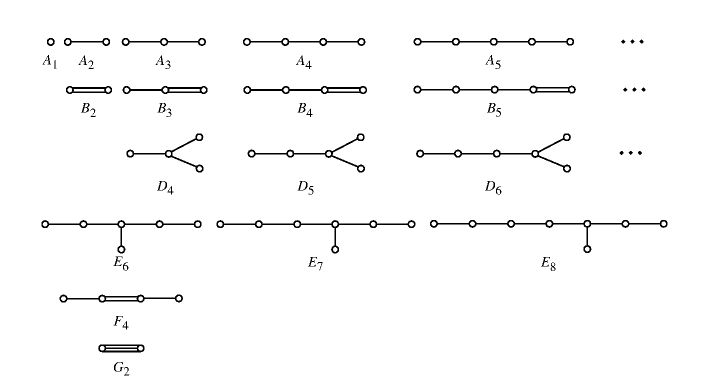
\includegraphics[scale =0.6]{chapters/dynkinDiagrams.png}
\end{center}
They are cleary connected and with at most 3 edges connecting each vertex. Now, we need to show that the associated 
quadratic form is positive definite. To do this, we look first at rank 2 Dynkin diagrams and observe that the associated Cartan 
matrices satisfies the Sylvester criterion. Now, for the remaning familes $A_l,B_l,D_l,\;l\geq3$ we apply an induction. 
To do this we observe that each such graph $\Gamma_l$ has a vertex with only one simple edge. We number this vertex by $l$ and the other vertex
connected to it we number by $l-1$. Therefore 
\begin{equation}
    \begin{split}
        \det(\Gamma_l)&=\det\begin{pmatrix}
        &&&&0\\
        &&&&\vdots\\
        &&&&0\\
        &&&2&-1\\
        0&\cdots&0&-1&2\\
    \end{pmatrix}\\
    &=2\det(\Gamma_{l-1})-(-1)\det\begin{pmatrix}
        \Gamma_{l-2}&0\\*&-1
    \end{pmatrix}\\
    &=2\det(\Gamma_{l-1})-\det(\Gamma_{l-2}).
    \end{split}
\end{equation}
where $\Gamma_{l-1},\Gamma_{l-2}$ are the Dynkin diagrams obteined by removing the vertex $l$ and $l,l-1$ respectively. By
taking the first cases we see that $\det(\Gamma_l)>0,\forall l\geq1$ for each family $A_l,B_l,D_l$. To the exceptional families 
we can do just an inspection.

\item Now we will construct another set of graphs called extended Dynkin diagrams. To do this, let $(V,\Delta)$ be a root 
system with simple roots $\Pi=\{\alpha_1,\dots,\alpha_l\}$. We define the extended Cartan matrix by 
\begin{equation}
    \widetilde{A}_{ij}=2\frac{(\alpha_i,\alpha_j)}{(\alpha_i,\alpha_i)},\;1\leq i,j\leq l+1
\end{equation}
where $\alpha_{l+1}=-\theta\;(\theta$ being the highest root). 
We define the associated extended Dynkin diagram in the same way. \par 
The extended Cartan matrix have similar properties of standard Cartan matrices. That is 
$\widetilde{A}_{ii}=2\;\forall i,  \widetilde{A}_{ij}\leq 0\;(i\neq j)$ 
and $0\leq  \widetilde{A}_{ij} \widetilde{A}_{ji}\leq 3\;(i\neq j)$. To see this, we observe that 
if $\theta$ is the highest root, then $(\theta,\alpha_i)\geq0\;\forall i$. By contradiction, suppose that this is not 
the case, i.e., there exist $i\;(1\leq i\leq l)$ such that $(\theta,\alpha_i)<0$. Since $\theta$ is maximal, we have 
$\theta+\alpha_i\notin\Delta_+$, so $q=0$. Therefore 
\begin{equation}
    0\leq p=2\frac{(\theta,\alpha_i)}{(\alpha_i,\alpha_i)}<0
\end{equation}
which is a contradiction. Furthermore, the inequality 
$0\leq 2\tfrac{(\theta,\alpha_i)}{(\alpha_i,\alpha_i)}\cdot2\tfrac{(\alpha_i,\theta)}{(\theta,\theta)}\leq 3$ follows from the fact 
that $\alpha_i,\theta\in\Delta$, so we have the string condition satisfied and 
$2\tfrac{(\theta,\alpha_i)}{(\alpha_i,\alpha_i)},2\tfrac{(\alpha_i,\theta)}{(\theta,\theta)}\in\bbZ$. Finally, this number is just 
$4\cos^2(\gamma)$, where $\gamma$ is the angle between $\theta$ and $\alpha_i$. Of course, since $\theta\notin\Pi\;(\#\Pi>1)$ we can not 
have $\gamma=0$.

\begin{dang}
    \begin{remark}
        Let $A\in M_n(\mathbb{F})$ be a $n\times n$ matrix over a field $\mathbb{F}$ and 
        $1\leq i_1\leq\cdots\leq i_r\leq n$. We define the corresponding principal minor of $A$ with respec to 
        $I=\{i_1,\dots, i_r\}$ by 
        \begin{equation}
            \det(A_{i_ki_l})_{1\leq k,l\leq r}
        \end{equation}
    \end{remark}
\end{dang}

Finally, we claim that all the principal minors of $\widetilde{A}$ are positive. First write 
\begin{equation}
    \widetilde{A}=\text{Diag}(\tfrac{2}{(\alpha_i,\alpha_i)})_{i=1}^{l+1}\cdot Q,\;Q= ((\alpha_i,\alpha_j))_{i,j=1}^{l+1}.
\end{equation}
Then for any subset $I\subset \{1,\dots,l+1\}$ of $l$ elemetns, the corresponding minor of $Q$ is the 
associated gram matrix of $(\cdot,\cdot)$ is some basis. So, by Silvester criterion, all of its leading minors are positive. Then we 
see that all principal minors of $\widetilde{A}$ are positive.




\begin{dang}
    \begin{example}
        Compute the extended Dynkin diagram for the Lie algebra $\fr{sl}_4$.
    \end{example}
\end{dang}
The roots are $\Delta=\{L_i-L_j:i\neq j\}\subset \bigoplus_{i=1}^4\bbC L_i$. The functional $f(L_i)=n+1-i$ yields the 
positive roots $\Delta_+=\{L_i-L_j: i< j\}$. So, in this case the simple roots are 
\begin{equation}
    \alpha_i=L_i-L_{i+1}, i=1,2,3
\end{equation}
while the maximal root is $\theta =\sum_i\alpha_i=L_1-L_4$. The extended Cartan matrix is 
\begin{equation}
    \begin{pmatrix}
        2&-1&0&-1\\
        -1&2&-1&0\\
        0&-1&2&-1\\
        -1&0&-1&2
    \end{pmatrix}
\end{equation}
with associated extended Dynkin diagram given by:
\begin{center}
    $
    \xymatrix{
        &\circ_3 \ar@{-}[rd] \ar@{-}[ld] &\\
        \circ_2 \ar@{-}[rd]&&\bullet_4 \ar@{-}[ld]\\
        &\circ_1&
    }$
\end{center}
Now, to see that $\det(\widetilde{A})=0$, we just observe that the last column is a linear combination of the previous collumns:
\begin{equation}
    \begin{split}
        C_{l+1} &= \begin{pmatrix}
        2\tfrac{(\alpha_1,\alpha_{l+1})}{(\alpha_1,\alpha_1)}\\2\tfrac{(\alpha_2,\alpha_{l+1})}{(\alpha_2,\alpha_2)}\\\vdots\\2
    \end{pmatrix}\\
    &= -\sum_{j=1}^lm_j
    \begin{pmatrix}
        2\tfrac{(\alpha_1,j)}{(\alpha_1,\alpha_1)}\\2\tfrac{(\alpha_2,\alpha_j)}{(\alpha_2,\alpha_2)}\\\vdots\\2\tfrac{(\alpha_{l+1},\alpha_j)}{(\alpha_{l+1},\alpha_{l+1})}
    \end{pmatrix}\\
    &=-\sum_jm_jC_j.
    \end{split}
\end{equation}
Next, follows the list all the extended Dynkind diagrams obtained using the above procedure for extension.
\begin{center}
    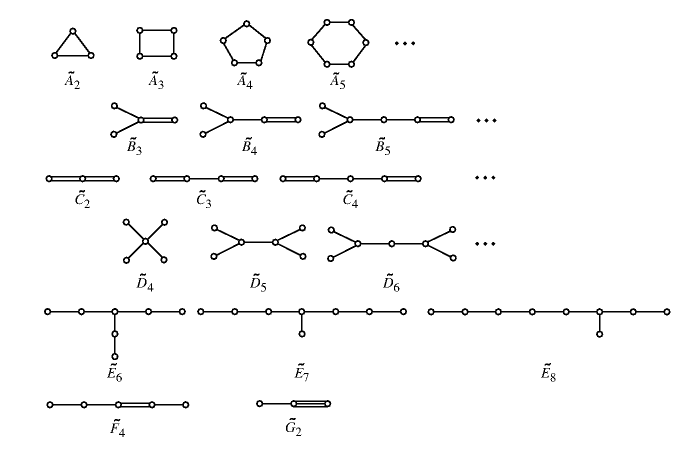
\includegraphics[scale=0.6]{chapters/extendedDynkinDiagrams.png}
\end{center}
\item  By the properties of extended Dynkin diagrams discussed before  
we see that any connected subgraph obtained from an extended Dynkin diagram by 
excluding vertices or decreasing the number of edges, satisfies the above properties of Dynkin diagrams: It's connected,
with at most 3 edges and the associated quadratic form is positive definite (recall the discussion of principal minors of 
an extended Cartan matrix).
\end{itemize}

\begin{dang}
    \begin{theorem}
        The Dynkin diagram of a simple Lie algebra is one of the ones: 
        \begin{equation}
            A_l,\;l\geq1;\;B_l,\;l\geq2;\;D_l,\;l\geq4;\; E_6 ;\; E_7 ;\;E_8;\; F_4;\; G_2.
        \end{equation}
    \end{theorem}
\end{dang}


\section{Cohomology}
\textit{Aplication}: To show that finite dimensional $\fr{g}-$modules, $\fr{g}$ semisimple, are completely reducible: If 
$A\subset B$ is a submodule, then there exist $C\subset B$ submodule such that $B\cong A\oplus C$. 

\begin{itemize}
    \item (\textbf{Main motivation}). Our initial step is to observe that if $A\subset B$ is a submodule, 
    then we have a complementary subspace $C$. That is, at the level of vector 
    spaces we have the splitting sequence: 
    \begin{center}
        \begin{tikzcd}
        0\arrow[r]&A\arrow[r, "i"]&B\arrow[r, "p"]&C\arrow[r]\arrow[l, bend left = 40, "s"]&0,\; p\circ s=\mathds{1}_{C}.
        \end{tikzcd}
    \end{center}
The point is: we do not know if $s$ is a map of $\fr{g}-$modules. In fact, we do not know even if $B$ is a $\fr{g}-$module.
\item(\textbf{Extensions}).  So we try the inverse path: Start with $\fr{g}-$modules $A,C$ and define the category of extensions 
of $C$ by $A$ as the set of exact sequences of $\fr{g}-$modules 
\begin{center}
      \begin{tikzcd}
        0\arrow[r]&A\arrow[r, "i"]&B\arrow[r, "p"]&C\arrow[r]&0
        \end{tikzcd}
\end{center}
Where morphisms between two sequences are defined by a $\fr{g}-$module morphism $f$  
such that the following diagram commutes:
\begin{center}
    \begin{tikzcd}
        0\arrow[r]\arrow[d, dashed]&A\arrow[r, "i"]\arrow[d,"\mathds{1}_A"]
        &B\arrow[d,"f"]\arrow[r, "p"]&C\arrow[r]\arrow[d,"\mathds{1}_C"]&0\arrow[d,dashed]\\
        0\arrow[r]&A\arrow[r, "i"]&B^\prime\arrow[r, "p"]&C\arrow[r]&0
    \end{tikzcd}
\end{center}
By the five lemma, $f$ is an isomorphism of vector spaces. 
\begin{dang}
    \begin{definition}
        We define $\Ext(C,A)$ as the set of isomorphisms classes of extensions of $C$ by $A$.
    \end{definition}
\end{dang}
\item(\textbf{Sections}). We know that if the exact sequence 
    \begin{center}
        \begin{tikzcd}
        0\arrow[r]&A\arrow[r, "i"]&B\arrow[r, "p"]&C\arrow[r]&0
        \end{tikzcd}
    \end{center}
splitts, then we have the $\fr{g}-$module morphism $B\cong A\oplus C$. By linear algebra, we know that there exist 
a linear map $s\in\Hom(C,B)$ such that $p\circ s=\mathds{1}_C$. So, we try to understand when the map 
\begin{equation}
    \xi_B:\fr{g}\to\Hom(C,A): x\mapsto[c\mapsto xs(c)-sx(c)]
\end{equation}
vanish. Observe that $\text{Im}(\xi_B)$ really lies in $A$, because 
\begin{equation}
    \begin{split}
        p\xi_B(x)&=pxs(c)-psx(c)\\
        &=xps(c)-psx(c)\\
        &=x(c)-x(c)\quad(\text{because }p\circ s=\mathds{1}_C)\\
        &=0.
    \end{split}
\end{equation}
So $\xi_B(x)\in\Ker(p)=\text{Im}(i)\cong A$. Observe that the morphism $\xi_B$ deppends on the choice of extension and 
the choice of splitting. Fix an extension and let $\xi_B,\xi_B^\prime$ be associated to two sections $s,s^\prime$. We have 
\begin{equation}
    (\xi_B-\xi_B^\prime)(x):c\mapsto x(s-s^\prime)c-(s-s^\prime)xc.
\end{equation} 
Then we see that $\xi_B-\xi_B^\prime$ comes from a map $\eta=s-s^\prime\in\Hom(C,A)$, because $p(s-s^\prime)=0$, that is 
$\text{Im}(s-s^\prime)\in\Ker(p)=\text{Im}(i)\cong A$.
\item(\textbf{Sistematization}). Lets try to sistematizate what we have done. Previously we constructed a kind of a ``map'':
\begin{center}
    \begin{tikzcd}
      \Hom(C,A)  &&  \Hom(C,A)\\
                 &\longrightarrow& \\
       \mathbb{F}\arrow[uu, "\eta"] &&  \mathbb{F}\arrow[uu, "\xi_B"]\arrow[uu,bend left=40,"\xi_B^\prime"]
    \end{tikzcd}
\end{center} 

\begin{dang}
   In the general framekork, we have:
\begin{equation}
    \begin{split}
        d: \Hom_{\bbF}(\bbF,M)&\;\longrightarrow \Hom_{\bbF}(\fr{g},M)\\
        m&\longmapsto [x\mapsto x\cdot m]
    \end{split}
\end{equation} 
\end{dang}

Moreover, we have the following observation: If $A,C$ are two $\fr{g}-$modules, $\Hom(C,A)$ also has 
a $\fr{g}-$module structure given by:
\begin{equation}
    (x\cdot f)(c)=xf(c)-f(xc).
\end{equation} 

So, by the previous discussion we have $\xi_B-\xi_B^\prime=d(\eta),\;\eta=s-s^\prime\in\Hom(C,A)$. 
Now we arrive at the main definition of this section.

\begin{dang}
    \begin{definition}
        (Chevalley-Eilenberg complex). Let $M$ be a $\fr{g}-$module and 
        $C^k(\fr{g},M)=\Hom_{\bbF}(\Lambda^k\fr{g},M)$. Define the map 
        \begin{equation}
            \begin{split}
                &d: C^k(\fr{g},M)\to C^{k+1}(\fr{g},M)\\
                &\quad df(x_1,\dots,x_{k+1})=
                \sum_{i=1}^k (-1)^{i+1} x_i\cdot f(x_1\wedge\cdots\wedge\widehat{x_i}\wedge\cdots\wedge x_{k+1})\\
                &\quad\quad\quad\quad +\sum_{i<j}(-1)^{i+j}
                f([x_i,x_j]\wedge x_1\wedge\cdots \wedge\widehat{x_i}\wedge\cdots\wedge\widehat{x_j}\wedge\cdots\wedge x_{k+1})
            \end{split}
        \end{equation}
        The Chevalley-Eilenberg complex is the complex $(C^k(\fr{g},M),d^k)$.
    \end{definition}
\end{dang}

In particular, we have 
\begin{equation}
    \begin{split}
        &d^0: C^0(\fr{g},M)\to C^1(\fr{g},M)\\
        &\;d^0(m)[x_1]=x_1\cdot m,\;m\in M\cong\Hom(\bbF,M)
    \end{split}
\end{equation}
and 
\begin{equation}
    \begin{split}
        &d^1:C^1(\fr{g},M)\to C^2(\fr{g},M)\\
    &\;d^1(f)[x_1\wedge x_2]=x_1f(x_2)-x_2f(x_1)-f([x_1,x_2])
    \end{split}
\end{equation}
\begin{dang}
    \begin{definition}
        We write $Z^n=\text{Ker}(d^n),\;B^n=\text{Im}(d^{n-1})$ and $H^n(\fr{g},M)=Z^n/B^n$.
    \end{definition}
\end{dang}

\item Now, coming back to extension of modules. Given an extension
\begin{equation}
    0\to A\overset{i}{\to}B\overset{p}{\to}C\to0
\end{equation}
 and the map 
$\xi_B\in\Hom(\fr{g},\Hom(C,A))$ constructed previously, we see that 
\begin{equation}
    d^1(\xi_B)(x\wedge y)=x\cdot\xi_B(y)-y\cdot\xi_B(x)-\xi_B([x,y])
\end{equation}
maps $c$ to 
\begin{equation}
    \begin{split}
        &x\cdot\xi_B(y)c-y\cdot\xi_B(x)c-\xi_B([x,y])c\\
        &\quad= x\xi_B(y)c-\xi_B(y)(xc)-y\xi_B(x)c+\xi_B(x)(yc)-\xi_B([x,y])c\\
        &\quad= xys(c)-xsy(c)-ysx(c)+syx(c)\\
        &\quad\quad-yxs(c)+ysx(c)+xsy(c)-sxy(c)-\xi_B([x,y])c\\
        &\quad=[x,y]s(x)-s([x,y]c)-\xi_B([x,y])c\\
        &\quad=0.
    \end{split}
\end{equation}
\begin{dang}
    \begin{remark}
        we must be careful here, we are using $\cdot$ to denote the action of $\fr{g}$ on $\Hom(C,A)$ !
    \end{remark}
\end{dang}

Therefore $\xi_B\in Z^1(\fr{g},\Hom(C,A))$. In particular, we see that the class
\begin{equation}
    [\xi_B]\in H^1(\fr{g},\Hom(C,A))
\end{equation}
is independent of the choice of the section $s$, in fact $\xi_B-\xi_B^\prime = d(s-s^\prime)$. 
So this class deppends only on the extension of $C$ by $A$.
\end{itemize}

Now we have all the tools to state the main theorems of this section. 
\begin{dang}
    \begin{theorem}
        The map $(0\to A\to B\to C\to 0)\mapsto [\xi_B]$ defines a bijection
        \begin{equation}
           \psi: \Ext(C,A)\overset{\cong}{\longrightarrow} H^1(\fr{g},\Hom(C,A))
        \end{equation}
    \end{theorem}
\end{dang}
Proof: First we show that this map is well defined. Suppose that we have an isomorphism $f:B\to B^\prime$ of 
exact sequences. That is $f$ is a $\fr{g}-$module isomorphism that makes the following diagram commutes:
\begin{center}
    \begin{tikzcd}
        0\arrow[r]\arrow[d, dashed]&A\arrow[r, "i"]\arrow[d,"\mathds{1}_A"]
        &B\arrow[d,"f"]\arrow[r, "p"]&C\arrow[r]\arrow[d,"\mathds{1}_C"]&0\arrow[d,dashed]\\
        0\arrow[r]&A\arrow[r, "i^\prime"]&B^\prime\arrow[r, "p^\prime"]&C\arrow[r]&0
    \end{tikzcd}
\end{center}
Choose sections $s\in\Hom(C,B),s^\prime\in\Hom(C,B^\prime)$ such that $ps=p^\prime s^\prime=\mathds{1}_C$. Here we need to be more 
formal with definitions. We have $\xi_B=i^{-1}\circ(xs-sx)$. Now we observe that 
\begin{equation}
   i^\prime\circ\xi_B(x)= fi\circ\xi_B(x)=x\circ fs-fs\circ x.
\end{equation}
Here we have used the hypothesis that $f$ is a $\fr{g}-$module morphism. Moreover, we have
\begin{equation}
    i^\prime\circ(\xi_B(x)-\xi_{B^\prime}(x))=x\circ(fs-s^\prime)-(fs-s^\prime)\circ x.
\end{equation}
However
\begin{equation}
    \begin{split}
        p^\prime(fs-s^\prime)&=p^\prime fs-p^\prime s^\prime\\
        &=ps-p^\prime s^\prime \\
        &=0.
    \end{split}
\end{equation}
Therefore $\text{Im}(fs-s^\prime)\subset\Ker(p^\prime)=\text{Im}(i^\prime)$. Since $i^\prime:A\to \text{Im}(i^\prime)$ is a 
$\fr{g}-$module isomorphism and $\text{Im}(fs-s^\prime)\subset\text{Im}(i^\prime)$, we have 
\begin{equation}
    \xi_B(x)-\xi_{B^\prime}(x)=d((i^\prime)^{-1}\circ(fs-s^\prime))\Rightarrow [\xi_B(x)]=[\xi_{B^\prime}(x)]\in H^1.
\end{equation}

Now we construct an inverse $\phi$ for this map. Let $\xi\in Z^1(\fr{g},\Hom(C,A))$, then we define a module structure on 
$A\oplus C$ given by $x(a,c)=(xa+\xi(x)c,xc)$. To show that this in fact defines a $\fr{g}-$module we use the fact that 
$d(\xi)=0$, that is 
\begin{equation}
    0=d(\xi)(x\wedge y)=x\cdot\xi(y)-y\cdot \xi(x)-\xi([x,y]).
\end{equation}
Then 
\begin{equation}
    \begin{split}
        [x,y](a,c)&=([x,y]a+\xi([x,y])c,[x,y]c)\\
        &=([x,y]a+x\cdot\xi(y)c-y\cdot \xi(x)c,[x,y]c)\\
        &=([x,y]a+x\xi(y)c-\xi(y)xc-y\xi(x)c+\xi(x)yc,[x,y]c).
    \end{split}
\end{equation}
But 
\begin{equation}
    \begin{split}
        xy(a,c)&=x(ya+\xi(y)c,yc)\\
        &=(xya+x\xi(y)c+\xi(x)yc,xyc).
    \end{split}
\end{equation}
So we see that $[x,y](a,c)=(xy-yx)(a,c)$. We claim that $Z^1\to\Ext(C,A)$ descends to a map $H^1\to \Ext(C,A)$. To see this 
we need to show that if $[\xi]=[\xi^\prime]$, then the associated modules $A\oplus C$ induced by $\xi$ and $\xi^\prime$ are 
isomorphic. First, we know that $\xi-\xi^\prime =d\lambda,\;\lambda\in\Hom(C,A)$. The linear isomorphism 
$\varphi_\lambda\in\End(C,A)$ which sends $(a,c)\mapsto (a+\varphi_\lambda(c),c)$ makes the diagram  
\begin{center}
     \begin{tikzcd}
        0\arrow[r]\arrow[d, dashed]&A\arrow[r, "i"]\arrow[d,"\mathds{1}_A"]
        &A\oplus C\arrow[d,"\varphi_\lambda"]\arrow[r, "p"]&C\arrow[r]\arrow[d,"\mathds{1}_C"]&0\arrow[d,dashed]\\
        0\arrow[r]&A\arrow[r, "i"]&A\oplus C\arrow[r, "p"]&C\arrow[r]&0
    \end{tikzcd}
\end{center} 
commutes. Furthermore, we have $x\cdot\varphi_\lambda = \varphi_\lambda\cdot x$ if and only if $\xi-\xi^\prime = d\lambda$. 
So $\varphi_\lambda$ is a $\fr{g}-$module isomorphism. Therefore, we have a well defined map $\phi:H^1\to\Ext(C,A)$.\par 

Finally, we show that $\psi\phi=\mathds{1}_{H^1}$ and $\phi\psi=\mathds{1}_{\Ext(C,A)}$. For the first one, we observe that
if we associate the corresponding module structure on $A\oplus C$ 
using $\xi_0\in Z^1$, then for any $c\in C$ we have
\begin{equation}
    i\circ \xi(x)c=x\circ s(c)-s\circ x(c)=x(0,c)-(0,xc)=(\xi_0(x)c,xc)-(0,xc)=(\xi_0(x)c,0)
\end{equation}
and $\xi(x)=\xi_0(x),\;\forall x\in\fr{g}$. Therefore $\psi\phi([\xi_0])=[\xi_0]$. Now, for the second identity, let 
$[\xi]=\psi(0\to A\overset{i}{\to} B\overset{p}{\to} C\to0)$, where $\xi=i^{-1}(x\circ s-s\circ x)$. To show that 
$\phi([\xi])=[0\to A\overset{i}{\to} B\overset{p}{\to} C\to0]$, we must find a $\fr{g}-$module morphism $f$ making 
the diagram 
\begin{center}
    \begin{tikzcd}
        0\arrow[r]\arrow[d, dashed]&A\arrow[r]\arrow[d,"\mathds{1}_A"]
        &A\oplus C\arrow[d,"f"]\arrow[r]&C\arrow[r]\arrow[d,"\mathds{1}_C"]&0\arrow[d,dashed]\\
        0\arrow[r]&A\arrow[r, "i"]&B\arrow[r, "p"]&C\arrow[r]&0
    \end{tikzcd}
\end{center}
commutes. There is no much of choice left: We try $f:A\oplus C\to B,\;f(a,c)=i(a)+\alpha s(c)$. So we see that, 
in order to the prevoius diagram commute, we need: $pf(a,c)=c\Rightarrow \alpha=1$. Furthermore $f(a,0)=i(a)$, so the previous 
diagram commutes and $f$ is an isomorphism by the 5 lemma. We need to show that $f$ is a $\fr{g}-$module morphism. We 
compute:
\begin{equation}
        xf(a,c)-f(xa+\xi(x)c,xc) 
        =xi(a)+xs(c)-i(xa)-i(\xi(x)c)-s(xc).
\end{equation}
But, $i$ is a $\fr{g}-$module morphism, so $i(xa)=xi(a)$, while $i(\xi(x)c)=xs(c)-sx(c)$ by definition.\qed

\begin{dang}
    \begin{theorem}
        (Whitehead lemma). If $\fr{g}$ is a semisimple Lie algebra and $V$ is a finite dimensional $\fr{g}-$module, then 
        $H^1(\fr{g},V)=0$.
    \end{theorem}
\end{dang}
Proof: The proof will be divided in several steps. 
\begin{itemize}
    \item[1.] Let $\fr{g}_0=\{X\in\fr{g}:Xv=0,\;\forall v\in V\}$, then $\fr{g}_0$ is an ideal. We claim that both 
    Lie algebras $\fr{g}_0, \overline{\fr{g}}=\fr{g}/\fr{g}_0$ are semisimple. To prove this we choose a basis 
    $\{X_1,\dots,X_k\}$ of $\fr{g}_0$ and extend it to a basis of $\fr{g}$ through the set $\{X_{k+1},\dots,X_n\}$. 
    It's a general property of semisimple Lie algebras that its ideals are also semisimple, so $\fr{g}_0$ is semisimple 
    (to see this, just define $\fr{a}=\fr{g}_0\cap(\fr{g}_0)^\perp$ and apply CC(sol) to see that it's a solvable ideal).
    So we just need to prove that $\overline{\fr{g}}$ is semisimple.\par 
    
    For $X,Y\in\fr{g}$ compute 
    \begin{equation}
        \begin{split}
            K^{\fr{g}}(X,Y)&=\Tr  
        \begin{pmatrix}
            X_{11}&X_{12}\\0&X_{22}
        \end{pmatrix}
        \begin{pmatrix}
            Y_{11}&Y_{12}\\0&Y_{22}
        \end{pmatrix}\\
        &=\Tr (X_{11}Y_{11})+\Tr (X_{22}Y_{22})\\
        &=\Tr (X_{11}Y_{11})+K^{\overline{\fr{g}}}(\overline{X},\overline{Y}).
        \end{split}
    \end{equation}
    The last line follows from the property that if $\ad(X)Z=Z_0+\sum_{i=k+1}^na_kX_k$, then 
$\ad(\overline{X})\overline{Z}=\sum_{i=k+1}^na_k\overline{X}_k$. 
Now, suppose that $K^{\overline{\fr{g}}}(\overline{X},\overline{Y})=0,\;\forall Y\in\fr{g}$ and let 
$X^\prime$ be the component of $X$ in $\fr{g}_0$. Then 
\begin{equation}
    K^{\fr{g}}(X^\prime,Y)=\Tr(X_{11}Y_{11})\Rightarrow K^{\fr{g}}(X-X^\prime,Y)=0,\forall Y\in\fr{g}.
\end{equation} 
Therefore, by CC(ss) we see that $X-X^\prime=0$, that is $X\in\fr{g}_0$.\par 
Now we observe that $\overline{\fr{g}}\hookrightarrow\End(V)$, so we can think $\overline{\fr{g}}\subset \End(V)$.
\item[2.] Next we show that $H^1(\fr{g},V)=0\iff H^1(\overline{\fr{g}},V)=0$. This shows that we can assume 
$\fr{g}\subset\End(V)$ without lost of generality. This follows from the following observation, if 
$f\in Z^1(\fr{g},V)$, then $f|_{\fr{g}_0}=0$. In fact, since $\fr{g}_0$ is semisimple, we have 
$[\fr{g}_0,\fr{g}_0]=\fr{g}_0$. So, for any $Z\in\fr{g}_0$ we can write $Z=[X,Y],\;X,Y\in\fr{g}_0$. However, since 
$f\in Z^1$, we have 
\begin{equation}
   f(Z)= f([X,Y])=Xf(Y)-Yf(X) = 0
\end{equation}
because $X,Y\in\fr{g}_0$. So $f$ descends to a map $\overline{f}:\overline{g}\to V$ and 
\begin{equation}
    \begin{split}
        f = d(\eta)&\iff f(X)=X\cdot\eta,\;\forall X\in\fr{g}\\
        &\iff \overline{f}(\overline{X})=\overline{X}\cdot\eta,\;\forall X\in\fr{g}\\
        &\iff \overline{f}=d(\eta).
    \end{split}
\end{equation}

\item[3.] From the previous observations we see that we can assume $\fr{g}\subset\End(V)$. The advantage of this hypothesis
is that we can apply CC(sol) using the trace form:
\begin{equation}
    (\fr{a},[\fr{a},\fr{a}])_V=0\iff \fr{a}\;\text{ is solvable}
\end{equation}
so the trace form is also nondegenerate. Then we can use it to construct dual basis and define the Casimir element.\par

Now, choose a dual basis $\{a_1,\dots,a_n\}$ and $\{b_1,\dots, b_n\}$ with respect to $(\;,\;)_V$. That is 
$(a_i,b_j)=\delta_{ij}$. We have the Casimir element 
\begin{equation}
    \Omega=\sum_{i=1}^na_ib_i\in Z(\mathcal{U}(\fr{g})).
\end{equation}
Decompose $V$ into generalized eigenspaces 
\begin{equation}
    V = \bigoplus_{\gamma\in\bbC}V_\gamma,\;V_\gamma= E_{\gamma}^{\Omega}.
\end{equation}
Since $\Omega\in Z(\mathcal{U}(\fr{g}))$, we see that each $V_\gamma$ is a submodule of $V$. Now we observe that 
$V_0\neq V$. In fact, if $V=V_0$, then $0=\Tr_V(\Omega)=\sum_i(a_i,b_i)=\dim(\fr{g})$, which is not the case. So, 
by defining $V^\prime = \bigoplus_{\gamma\in\bbC^*}V_\gamma$, we see that $V=V^\prime\oplus V_0$ with 
$\dim(V_0),\dim(V^\prime)<\dim(V)$. The result will follow by induction on dimension of $V$ provided we show that 
\begin{dang}
    \begin{equation}
    \begin{aligned}
        &(a)\; H^1(\fr{g},V^\prime)=0\\
        &(b) \text{ By (a), we have } H^1(\fr{g},V)\cong H^1(\fr{g},V_0).
    \end{aligned}
\end{equation}
\end{dang}
We will prove $(a)$ on the next item. Assume it for now and lets show that its implies the second item. We have a 
natural homomorphism
\begin{equation}
    \psi: H^1(\fr{g},V_0)\rightarrow H^1(\fr{g},V).
\end{equation}
We claim that under the condition $H^1(\fr{g},V^\prime)=0$, this is an isomorphism. First we show injectivity: if 
$\psi([\xi])=0$, then there exist $\eta\in V$ such that $\xi=d(\eta)$. To show that $[\xi]=0$ in $H^1(\fr{g},V_0)$, we 
need to show that we can take $\eta\in V_0$. 
To see this, write $\eta=\sum_{\gamma\in S}\eta_{\gamma},\;\eta_{\gamma}\in V_{\gamma}$. Then, since each $V_{\gamma}$ is a 
submodule, we have $x\cdot\eta =\xi(x)\in V_0\iff x\cdot\eta=x\cdot \eta_0$, so $\xi=d(\eta_0)$ and $[\xi]=0$ in 
$H^1(\fr{g},V_0)$. Now we prove that $\psi$ is surjective, let $[\xi]\in H^1(\fr{g},V)$, so 
$\xi\in Z^1(\fr{g},V)$. The projection $p:V\to V^\prime$ is a $\fr{g}-$module homomorphism. Moreover, we claim that 
$p\xi\in Z^1(\fr{g},V^\prime)$. This follows from the calculation 
\begin{equation}
    \begin{split}
        d(p\xi)[X\wedge Y]&=Xp\xi(Y)-Yp\xi(X)-p\xi([X,Y])\\
        &=pX\xi(Y)-pY\xi(X)-p\xi([X,Y])\quad(p \text{ is a module morphism})\\
        &=p(X\xi(Y)-Y\xi(X)-\xi([X,Y]))\\
        &=pd(\xi)[X\wedge Y]\\
        &=0.
    \end{split}
\end{equation}
Now we use the hypothesis that $H^1(\fr{g},V^\prime)=0$ to see that this implies that $p\xi=d(\eta),\;\eta\in V^\prime$. 
Also, observe that $pd(\eta)(x)=p(x\cdot \eta)=x\cdot \eta$ because $V^\prime$ is invariant by the $\fr{g}$ action. So 
we see that $p\circ (\xi-d(\eta))=0\Rightarrow \text{Im}(\xi-d(\eta))\subset V_0$. So we can write the class 
$[\xi-d(\eta)]\in H^1(\fr{g},V_0)$ which is clearly mapped to $[\xi]$ through $\psi$. This proves the claim.

\item[4.] Now we prove that $H^1(\fr{g},V^\prime)=0$. To show this, we need a lemma.
\begin{dang}
    \begin{lemma}
        We have the following identity:
        \begin{equation}
            X\cdot(\sum_i a_i\xi(b_i))=\Omega\circ \xi(X).
        \end{equation}
    \end{lemma}
\end{dang}
Proof: This follows form the calculation
\begin{equation}
    \begin{split}
         X\cdot(\sum_i a_i\xi(b_i))&=\sum_i Xa_i\xi(b_i)\\
         &=\sum_i([X,a_i]\xi(b_i)+a_iX\xi(b_i))\\
         &=\sum_i([X,a_i]\xi(b_i)+a_ib_i\xi(X)+a_i\xi([X,b_i]))\quad(\text{because }\xi\in Z^1)\\
         &=\sum_i([X,a_i]\xi(b_i)+a_i\xi([X,b_i]))+\Omega\circ\xi(X)\quad(\text{definition of }\Omega)\\
         &=\sum_{i,j}(([X,a_i],b_j)a_j\xi(b_i)+([X,b_i],a_j)a_i\xi(b_j))+\Omega\circ\xi(X)\\
         &=\sum_{i,j}(([X,a_i],b_j)a_j\xi(b_i)+([X,b_j],a_i)a_j\xi(b_i))+\Omega\circ\xi(X)\\
         &=\sum_{i,j}(([X,a_i],b_j)+([X,b_j],a_i))a_j\xi(b_i)+\Omega\circ\xi(X)\\
         &=\Omega\circ\xi(X).
    \end{split}
\end{equation}
The last line follows by invariance of $(\;,\;)_V$. Now, the proof of the claim becomes easy. Let 
$\xi\in Z^1(\fr{g},V^\prime)$, then $\Omega\circ \xi(X)=X\cdot v_0$ where $v_0=\sum_i a_i\xi(b_i)\in V_0$. However, 
$\Omega|_{V^\prime}$ is invertible, so we can write $\xi(X)=\Omega^{-1}(X\cdot v_0)=X\cdot(\Omega^{-1}(v_0))$. Therefore 
\begin{equation}
    \xi = d(\Omega^{-1}(v_0))
\end{equation}
and $[\xi]=0$.
\end{itemize}
\qed
\begin{dang}
    \begin{corollary}
        Each finite dimensional $\fr{g}-$module is completely decomposable.
    \end{corollary}
\end{dang}
Proof: Let $A\subset B$ an invariant subspace. So we have an exact sequence $(0\to A\to B\to C\to 0)\in \Ext(C,A)$, where 
$C=B/A$. Since $H^1(\fr{g},\Hom(C,A))=0$, we get an isomorphism $B\cong A\oplus C$, where the module structure of 
$A\oplus C$ comes from the zero class $[0]\in H^1$, that is $x(a,c)=(xa,xc)$.\qed



